\documentclass[11pt,a4paper]{article}
\usepackage[utf8]{inputenc}
\usepackage[T1]{fontenc}
\usepackage{amsmath,amsfonts,amssymb}
\usepackage{graphicx}
\usepackage{subcaption}
\usepackage{booktabs}
\usepackage{geometry}
\usepackage{hyperref}
\usepackage{float}
\usepackage{listings}
\usepackage{xcolor}
\usepackage{titling}

\geometry{margin=2cm}

\setlength{\droptitle}{-2cm}

\hypersetup{
    colorlinks=false,
    pdfborder={0 0 0},
}

\lstset{
    basicstyle=\ttfamily\small,
    breaklines=true,
    frame=single,
    backgroundcolor=\color{gray!10}
}

\title{Riding Wavelets: Data-Mining Fundamental Knowledge in Financial Time Series - MVA 2025/26}
\author{Janis Aiad janisaiad.ja@gmail.com, Jordi Baroja baroja.jordi@gmail.com}
\date{\today}

\begin{document}

\maketitle



% \begin{abstract}
% This report documents the reproduction of the methodology described in ``Riding Wavelets: A Method to Discover New Classes of Price Jumps'' by Aubrun et al. We implement the wavelet-based feature extraction and Kernel PCA for jump classification, analyze the distribution of jump scores, and compare results with and without Scattering Spectra features. Our implementation is tested on multiple datasets including Poland and Hong Kong stock markets.
% \end{abstract}

\section{Introduction}



Financial datasets record stock prices of multiple assets over time and constitute a primary source for studying financial markets and their behavior. The data are extreme and highly non-stationary across all scales, from minutes to days. The features to be extracted are therefore very difficult to identify and are not publicly disclosed by hedge funds.
Non-stationarity makes dictionary learning unstable, so we instead rely on analyses based on spectral features. According to the paper, applying PCA in the wavelet space successfully captures these features using data from multiple jumps across financial markets.\\

This report presents our open source implementation \href{https://github.com/janisaiad/timeseries}{https://github.com/janisaiad/timeseries} of the jump detection and classification methodology proposed by Aubrun et al.~\cite{aubrun2024ridingwaveletsmethoddiscover}. The paper introduces an unsupervised framework based on wavelet coefficients to classify financial price jumps according to their reflexivity, mean-reversion, and trend-alignment properties.\\

\textbf{Our implementation is based on code developed from scratch and public findable, accesible, interpretable, reusable data available at~\cite{stooqDB}}, and tests the methodology across different countries and sampling frequencies. The jump detection and wavelet transformation code was developed by Janis Aiad, while Jordi Baroja focused on hyperparameter testing and finding correlations between features. Both authors fully understood all aspects of the paper, ran numerical experiments, and drew conclusions jointly.

% Our implementation includes:
% \begin{itemize}
%     \item Jump detection using 4-sigma threshold on standardized returns
%     \item Wavelet scattering coefficient extraction
%     \item Kernel PCA for dimensionality reduction
%     \item Classification into endogenous, exogenous, and anticipatory jumps
%     \item Analysis of mean-reversion and trend directions
%     \item Comparison with and without Scattering Spectra features
% \end{itemize}

\section{Method}


\subsection{Jump Detection}

Following the paper's methodology, we compute the log returns for a given stock price time series as 
$r(t) = \log\left(\frac{P(t+1)-P(t)}{P(t)}\right)$. While the data in the paper is recorded every 1 minute, we also work with 5-minute, hourly, and daily data. The normalization of the data is performed as follows:

\begin{equation}
x(t) = \text{sign}\left(\frac{r(0)}{f(0)\sigma(0) }\right)\frac{r(t)}{f(t)\sigma(t) } \quad\text{Forcing $x(0) > 0$}
\end{equation}
The term $f(t)$ represents the intraday volatility pattern (U-shape), computed as the median of returns at each time of day for a given stock across multiple days, and normalized to have unit quadratic mean. The term $\sigma(t)$ is the exponentially weighted moving standard deviation (EWMA), which computes the standard deviation of past values with exponential decay. We changed this estimator since it produces better results than the one the paper uses.  
As stated in the paper~\cite{aubrun2024ridingwaveletsmethoddiscover}, under the null hypothesis of Gaussian residuals (no-jump hypothesis), $|x(t)|$ converges towards a Gumbel distribution.\\

Theoretically, jumps are detected when $|x(t)| > 3.95$, corresponding to a 4-sigma deviation. We filter trading hours to exclude the first and last 60 minutes of each trading day (10:30-15:00 window).

\subsection{Wavelet Feature Extraction}

We implement the wavelet scattering representation $\Phi(x)$. For that, we use a complex wavelet filter $\psi(t)$ wose Fourier transform is real, has 0 average and the real part is even while the imaginary part is odd. Several functions exist with those properties and are well established to be good at feature extraction and can be found in (\text{PyWavelets})~\cite{pywt}.

\begin{itemize}
    \item Primary coefficients: \[
W_j x(t) := x \star \psi_j(t), \quad j \in \{1,\ldots,J\}, \quad \text{where } \star \text{ denotes convolution and } \psi_j(t) = \psi(2^{-j} t).
\] This leads to $2J$ coefficients, as we save the real and imaginary part evaluated at $t=0$.
    \item Second-order coefficients: \[
W_{j_2} \, |W_{j_1} x|(t) := \big| x \star \psi_{j_1} \big| \star \psi_{j_2} (t), \quad 
1\leq j_1 < j_2 \leq J, \quad \text{where } |\cdot| \text{ denotes the absolute value.}
\] This yields $J(J-1)$ coefficients since we save $J\choose 2$ imaginary and real coefficients evaluated again at 0.
\end{itemize}

For $J=6$ scales, this yields 42 features represenation so $\Phi(x)\in\mathbb{R}^{42}$. Recall that every normalized jump $x$ has $T$ components, being $x_0$ the moment of the jump and saving log returns from $x_{-T//2}$ until $x_{T//2}$. In our case $T=25$. 

\subsection{Scattering Spectra}

We also implement the Scattering Spectra (SS) features as described in Morel et al.~\cite{morel2022scale}:
\begin{itemize}
    \item $\Phi_1[j]$: Low-moment kurtosis measure, $\Phi_2[j]$: Average volatility at scale $2^j$
    \item $\Phi_3[j,j']$: Multi-scale skewness (complex), $\Phi_4[j_1,j'_1,j_2]$: Multi-scale kurtosis via second-order scattering (complex)
\end{itemize}

\subsection{Kernel PCA and Classification}

After we compute the wavelet and scattering spectra representation of each processed jump $x$, we apply Kernel PCA (RBF kernel, linear kernel) to obtain a low-dimensional embedding. The first principal component $D_1$ captures volatility asymmetry (reflexivity). We also compute handcrafted features:
\begin{itemize}
    \item $D_2$: Mean-reversion = $x(-1) - x(+1)$
    \item $D_3$: Trend = $x(-1) + x(+1)$
    \item Asymmetry: \[
A_{\text{jump}} = \frac{A_> - A_<}{A_> + A_<}, \quad 
\text{where } A_{</>} := \sum_{t_{</>}0} \big| x(t) - \min_{t_{</>}0} x(t) \big|
\]
\end{itemize}

\subsection{Description of experiments}
In the experiments we conduct, we focus on testing whether including scattering spectra features improves classification. We also compare different KPCA methods (RBF and Linear), vary the J value in the wavelet representation, and perform tests across different countries to see if PCA captures the same features.
Additionally, we examine the relationship between learned features and hand-crafted features-a comparison not performed in the original paper—using different timescales and plotting feature quantiles to visualize the extracted patterns.

\section{Data}

We use open source \href{https://stooq.com}{Stooq} OHLC data for multiple stock markets and multiple sampling frequencies (5-min, hourly, daily; see Tables~\ref{tab:data_poland}). Since the original paper uses 1-minute data with a 119-point window and $J=6$, we adapt to coarser bars with shorter windows and set $J=3$ for 5-min experiments.

\begin{table*}[t]
\centering
\scriptsize
\setlength{\tabcolsep}{4pt}
\renewcommand{\arraystretch}{1.15}
\begin{tabular}{lrrrll}
\toprule
freq & $n$ stocks & total points & span (days) & start & end \\
\midrule
5min   & 80 & 477302 & 148   & 07/07/2025 10:00 & 12/02/2025 15:40 \\
hourly & 80 & 105700 & 628   & 04/11/2024 11:00 & 12/30/2025 16:00 \\
daily  & 80 & 254918 & 10205 & 01/21/1998       & 12/30/2025 \\
\bottomrule
\end{tabular}
\caption{Poland dataset summary (after preprocessing).}
\label{tab:data_poland}
\end{table*}

% \begin{table*}[t]
% \centering
% \scriptsize
% \setlength{\tabcolsep}{4pt}
% \renewcommand{\arraystretch}{1.15}
% \begin{tabular}{lrrrll}
% \toprule
% freq & $n$ stocks & total points & span (days) & start & end \\
% \midrule
% 5min   & 23 &  52081 & 147   & 06/10/2025 10:00 & 11/04/2025 15:55 \\
% hourly & 35 &  44143 & 572   & 04/11/2024 11:00 & 11/04/2025 16:00 \\
% daily  & 30 & 109233 & 11849 & 05/27/1993       & -- \\
% \bottomrule
% \end{tabular}
% \caption{Hungary dataset summary (after preprocessing).}
% \label{tab:data_hungary}
% \end{table*}

\subsection*{Preprocessing diagnostics: jump-score distribution and tails}
The standardized returns exhibit heavy tails; the upper tail of $|x(t)|$ is well captured by a Gumbel fit on a high-quantile range, consistent with the max-stable null model discussed in the paper. We aggregate 12$\times$5-min bars into hourly and 12$\times$hourly into daily; since the number of observations (and thus extreme events) decreases sharply at coarser scales, we use lower practical thresholds at coarser frequencies (roughly $\tau\approx4$ for 5-min, $\tau\approx3$ for hourly, $\tau\approx2$ for daily) to retain enough jumps for stable statistics. We note that the 5-min tail shows a mild deviation from the Gumbel fit in the far tail; this could indicate a heavier-than-exponential tail (suggesting a Fr\'echet/GEV-type behavior) rather than a pure Gumbel regime, but we do not push this interpretation further here. We also note that our volatility estimator was adjusted during development; a deeper extreme-value analysis (e.g., GEV/GPD fits on exceedances) is left for future work.

\begin{figure}[H]
\centering
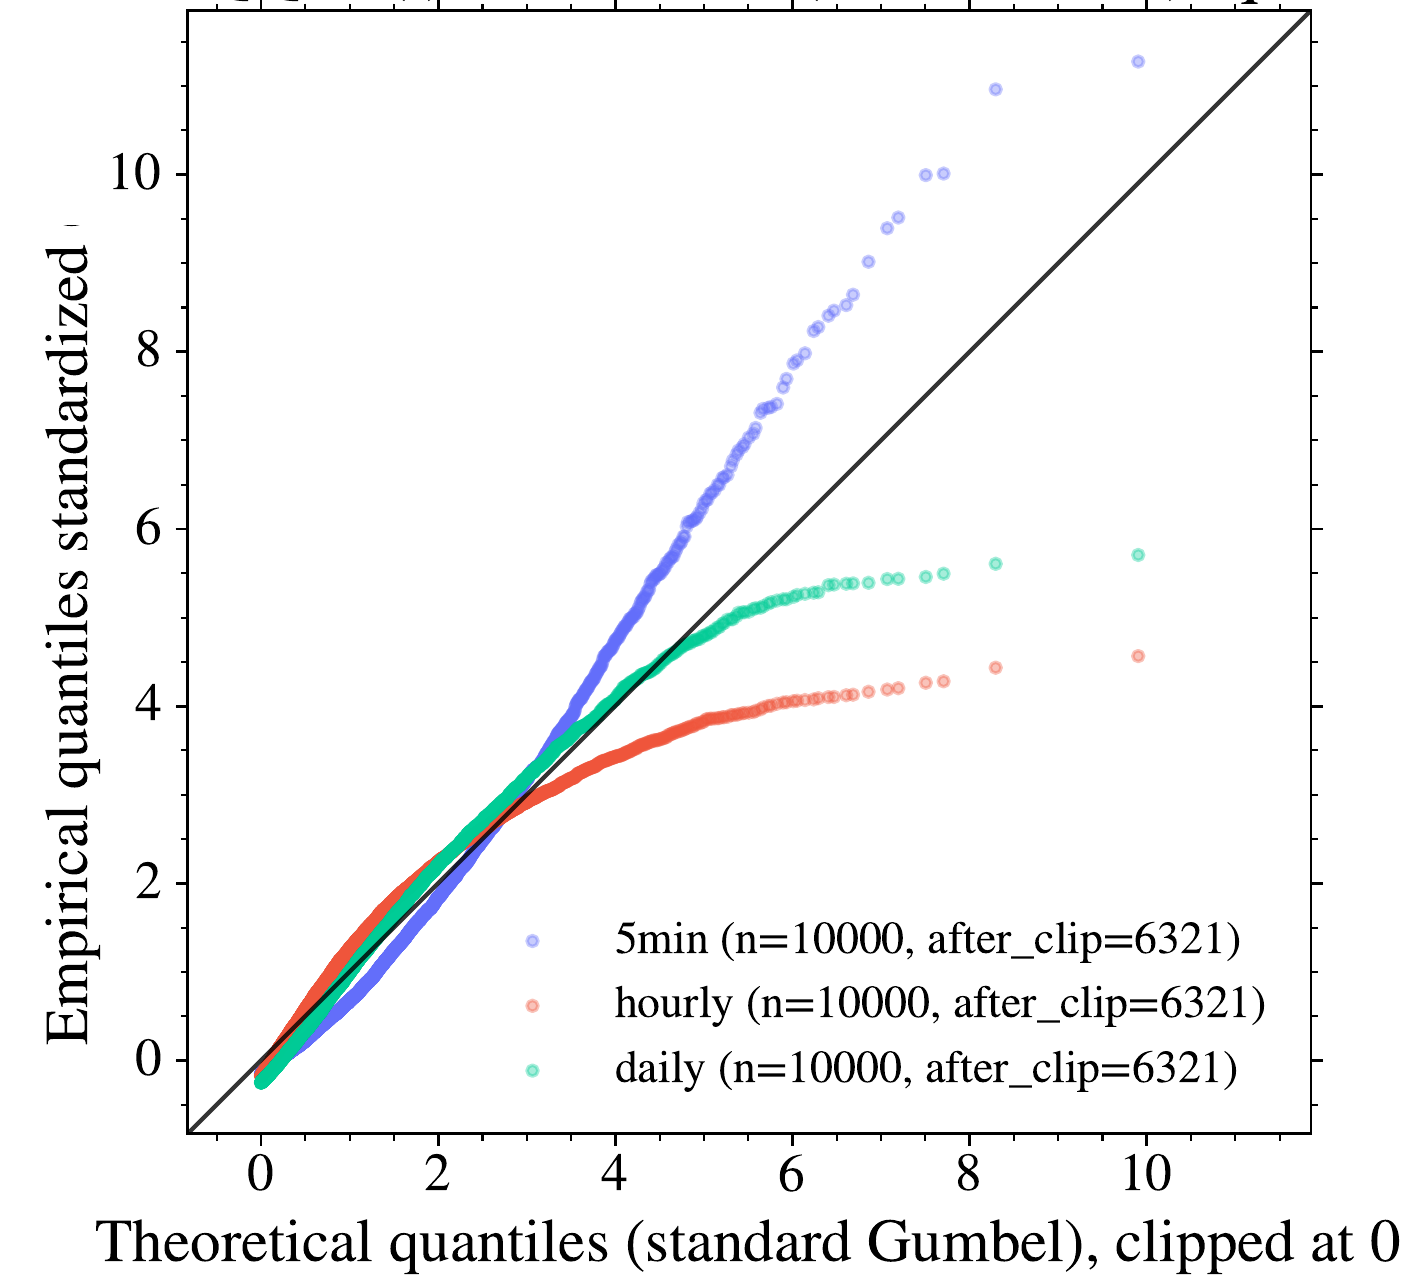
\includegraphics[width=0.3\linewidth]{figures/2/qq_abs_score_vs_gumbel_STACKED_mpl.png}
\caption{Q--Q plot of $|x(t)|$ against the fitted Gumbel distribution (stacked across 5-min, hourly, daily).}
\label{fig:poland_gumbel}
\end{figure}

\begin{figure*}[t]
\centering
\begin{subfigure}{0.48\textwidth}
    \centering
    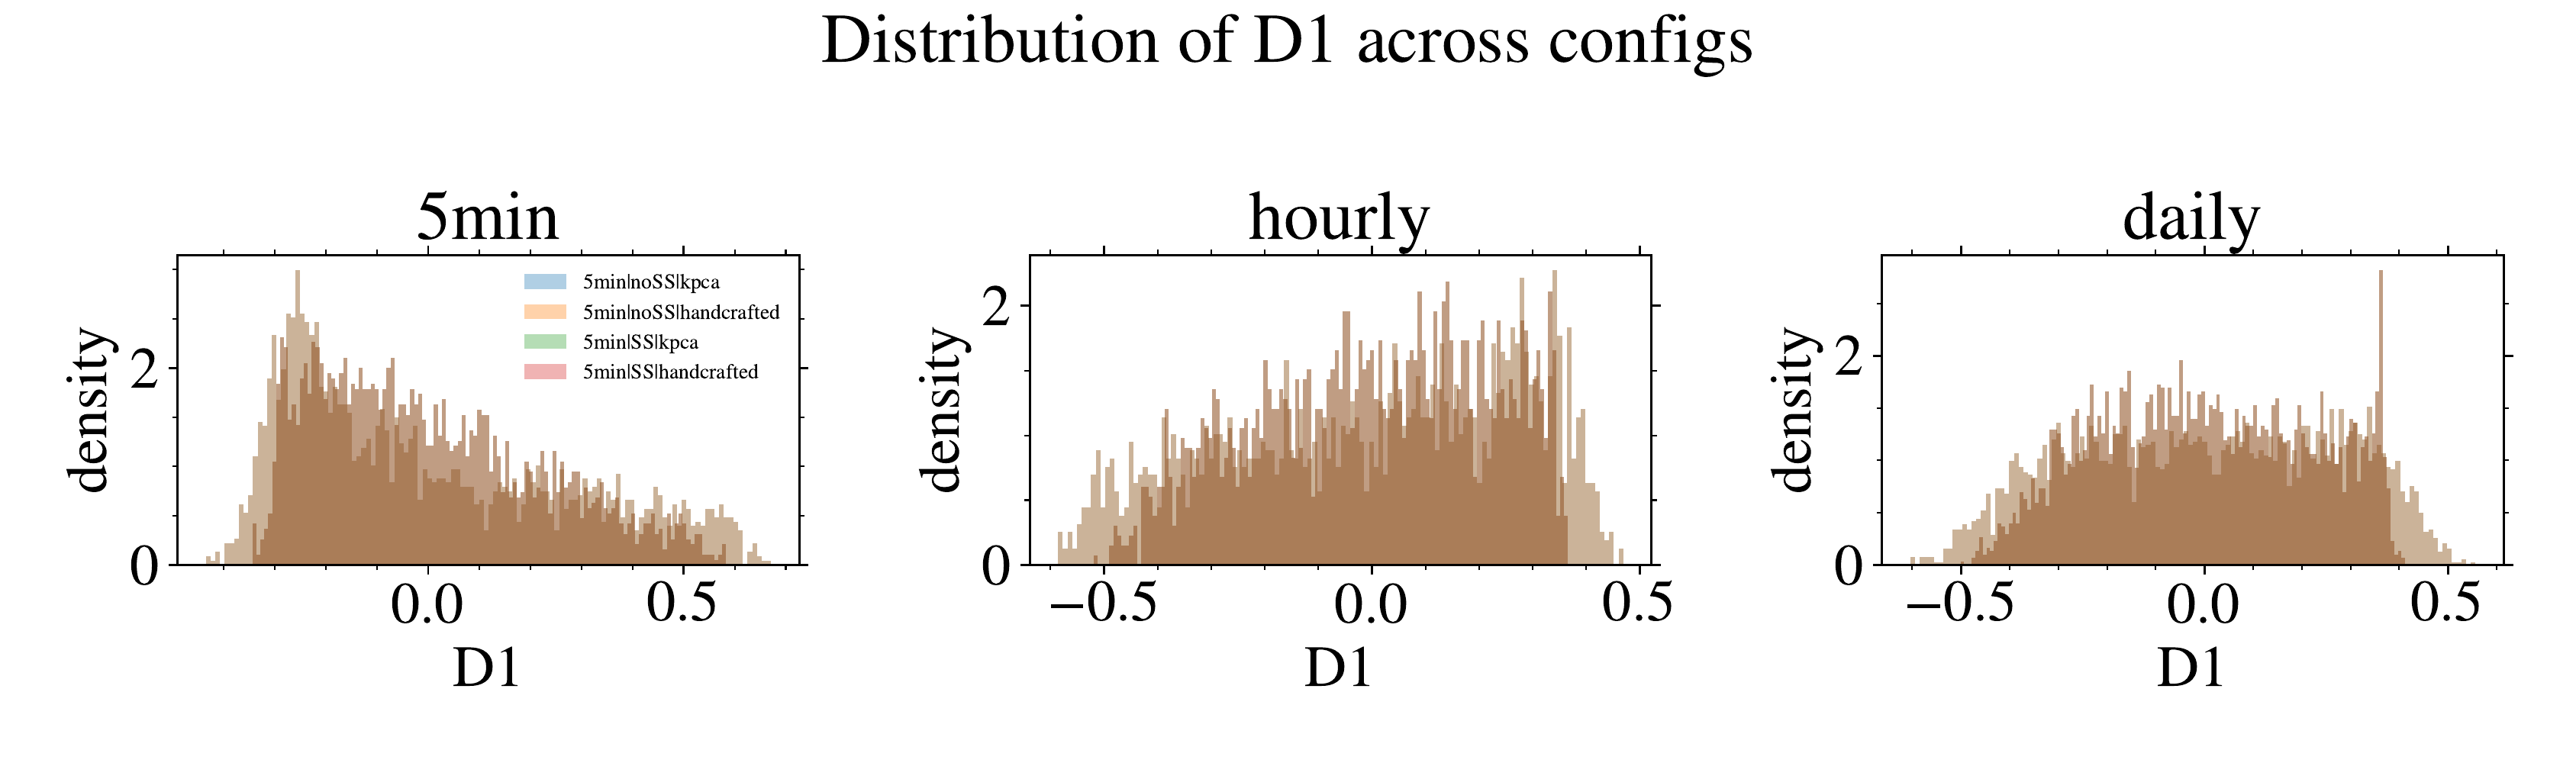
\includegraphics[width=\textwidth]{figures/2/hist_D1_mpl.png}
    \caption{Distribution of $D_1$ (linear scale).}
\end{subfigure}
\begin{subfigure}{0.48\textwidth}
    \centering
    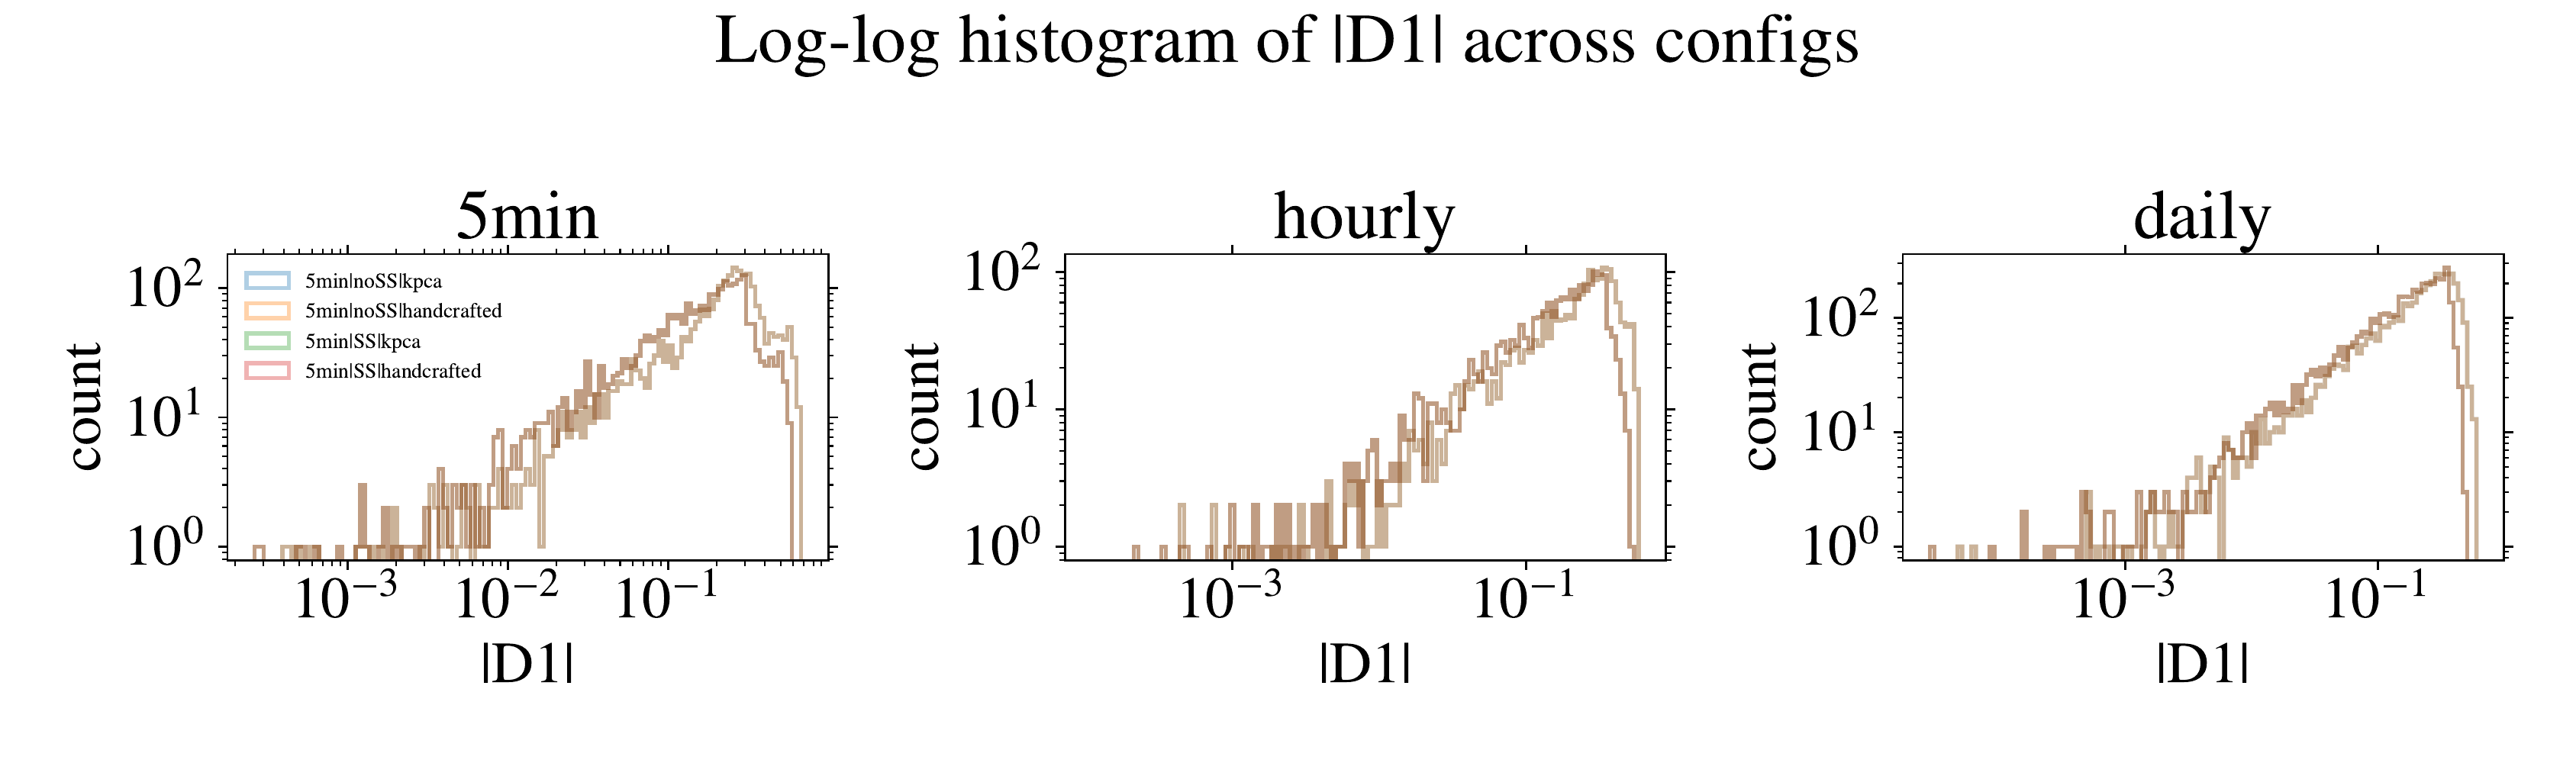
\includegraphics[width=\textwidth]{figures/2/hist_abs_loglog_D1_mpl.png}
    \caption{Distribution of $|D_1|$ (log--log).}
\end{subfigure}
\begin{subfigure}{0.48\textwidth}
    \centering
    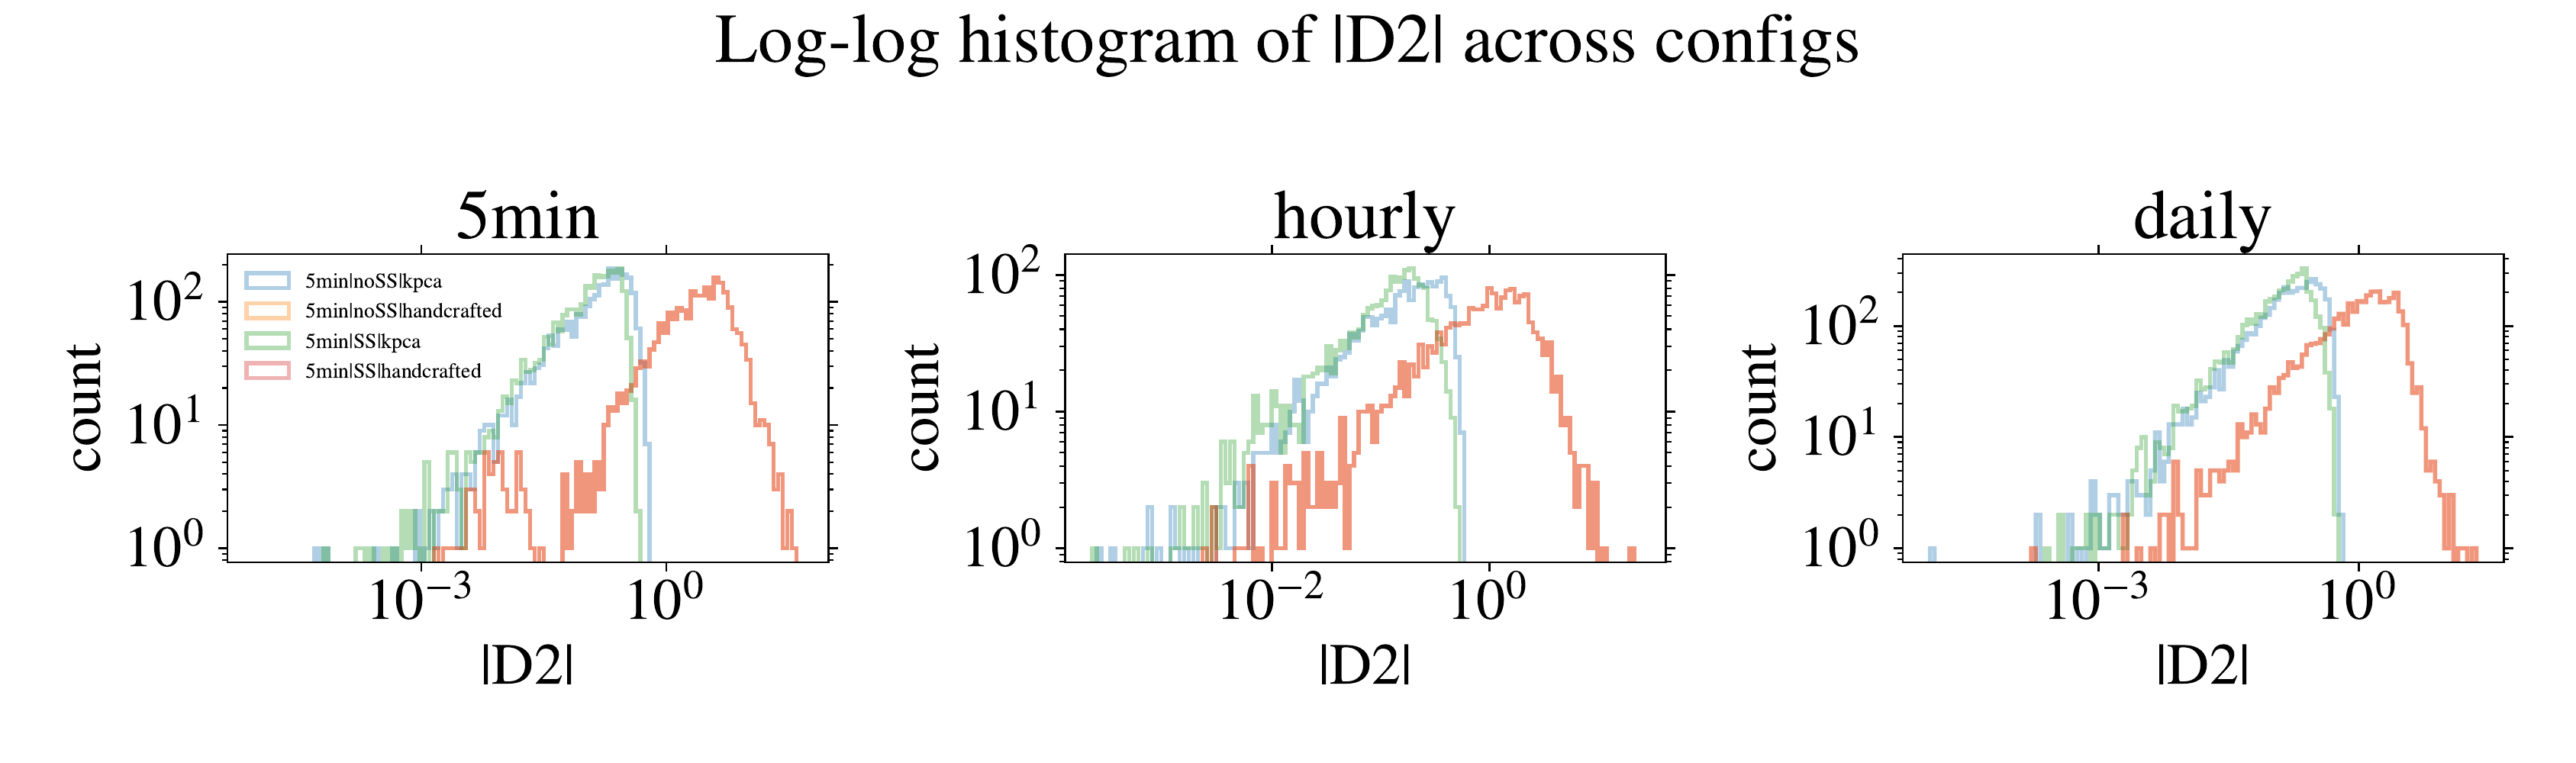
\includegraphics[width=\textwidth]{figures/2/hist_abs_loglog_D2_mpl.png}
    \caption{Distribution of $|D_2|$ (log--log).}
\end{subfigure}
\begin{subfigure}{0.48\textwidth}
    \centering
    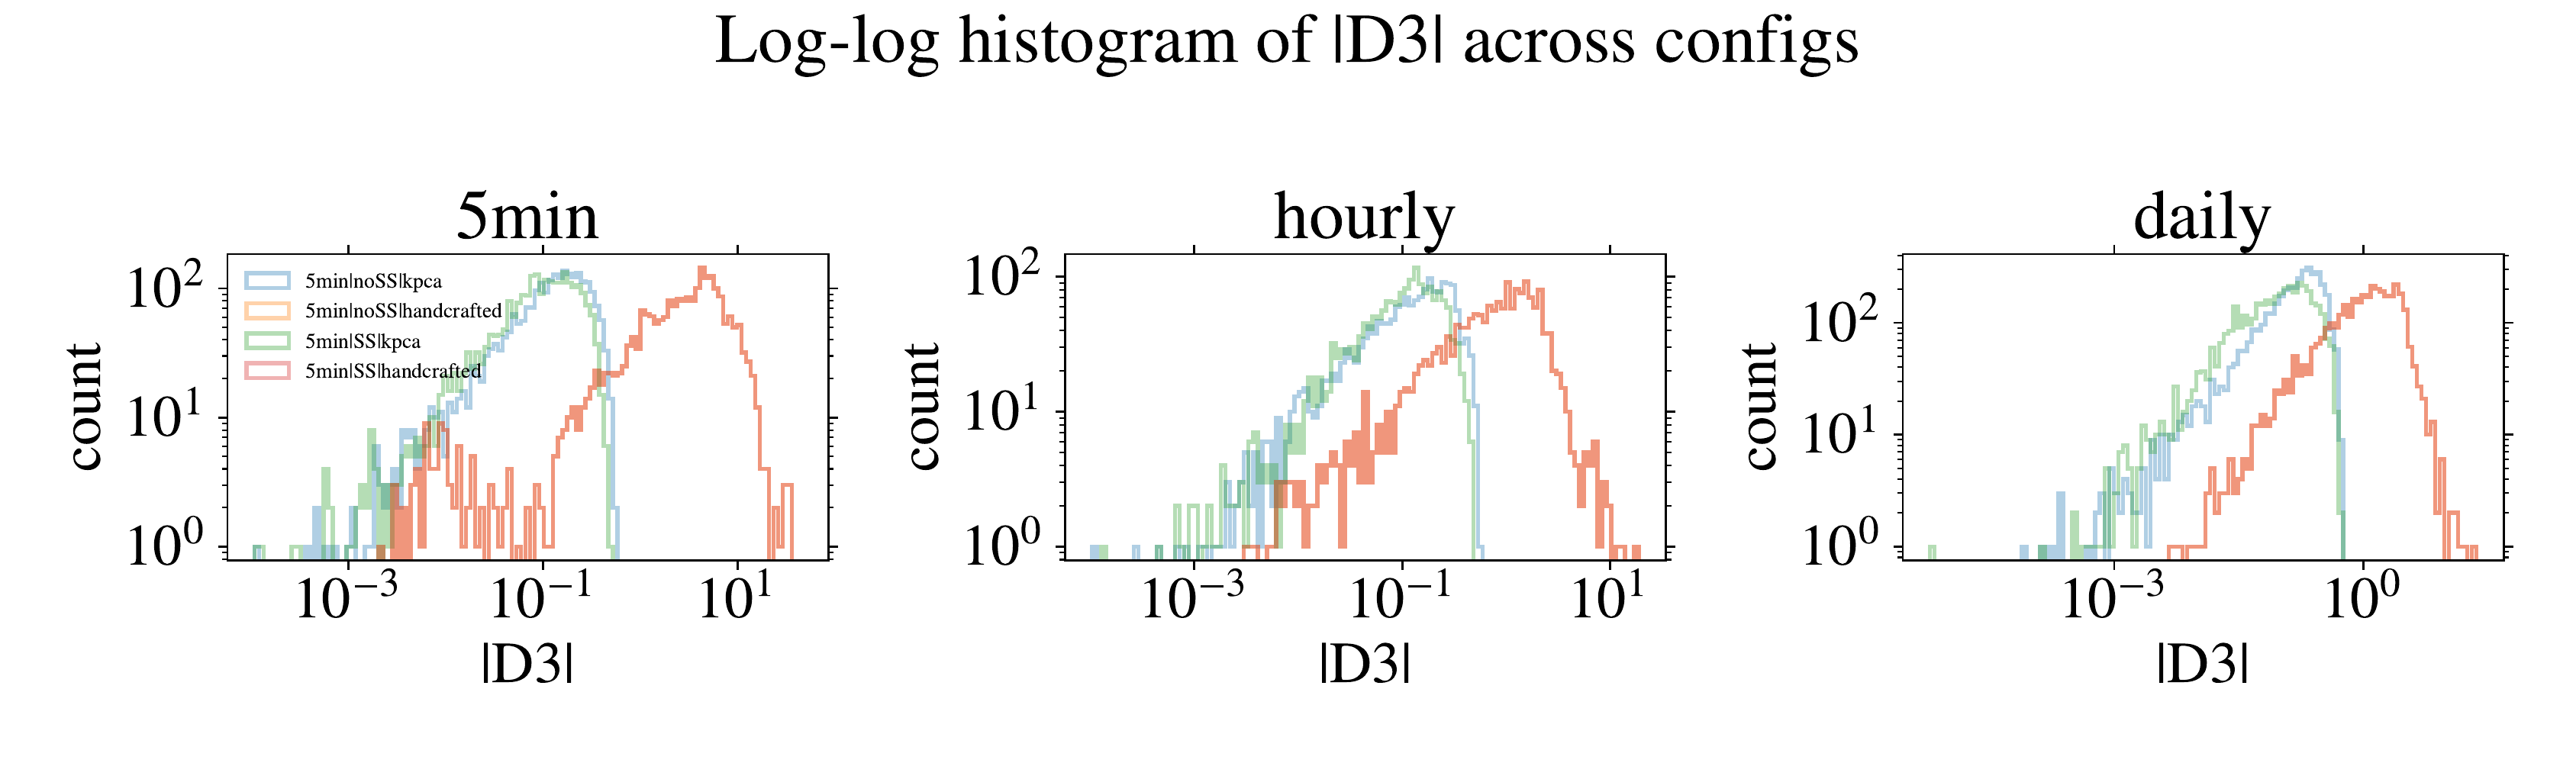
\includegraphics[width=\textwidth]{figures/2/hist_abs_loglog_D3_mpl.png}
    \caption{Distribution of $|D_3|$ (log--log).}
\end{subfigure}
\caption{Distribution diagnostics (Poland, 5-min): reflexivity score $D_1$ and tails of $|D_1|,|D_2|,|D_3|$.}
\label{fig:score_distributions}
\end{figure*}

\paragraph{Data conclusion.}
Overall, the preprocessing checks support the hypotheses needed for the wavelet pipeline: after de-seasonalization and volatility normalization, jump scores have stable heavy-tail behavior compatible with the paper's extreme-value motivation, and the learned directions exhibit well-behaved empirical distributions. This gives confidence that applying the embedding and interpretability analysis below is meaningful on our datasets.

\section{Results}

% \subsection{Recovered directions: reflexivity, mean-reversion, trend}
% We recover the key qualitative structure of the paper: $D_1$ captures volatility time-asymmetry (reflexivity), while $D_2$ and $D_3$ capture short-term mean-reversion and trend behaviors. The distributional diagnostics for $|x(t)|$ (Gumbel Q--Q) and for the learned scores ($D_1$ and the tails of $|D_1|,|D_2|,|D_3|$) are reported in the Data section as preprocessing checks.

% Projecting onto $(D_1,D_2)$ and $(D_1,D_3)$ separates interpretable behaviors (mean-reversion and trend). Due to the strict page limit and focus on robustness, we report the 2D projections qualitatively and focus on the score distributions and threshold sweeps shown in \ref{fig:threshold_sweep_5min}.




\subsection{Hyperparameter test}

\textbf{Ablation: Scattering Spectra features}
Adding SS features yields very similar $D_1$ embeddings (high correlation), suggesting that the base wavelet scattering coefficients already capture the dominant reflexivity signal at this resolution. \\

\textbf{Robustness to the jump threshold (5-min)}
We evaluate the sensitivity of the discovered directions to the jump-detection threshold $\tau$. For 5-min data, we observe a striking stability across thresholds (e.g., $\tau\in[2.5,4.5]$): $D_1$ and $D_3$ profiles are nearly unchanged, while $D_2$ can degrade slightly at the most extreme thresholds due to a small set of outliers that do not follow the typical mean-reversion pattern.
Supplementary overlays for hourly and daily data are provided in \ref{fig:threshold_sweep_5min}.\\

\begin{figure*}[t]
\centering
\begin{subfigure}{0.32\textwidth}
    \centering
    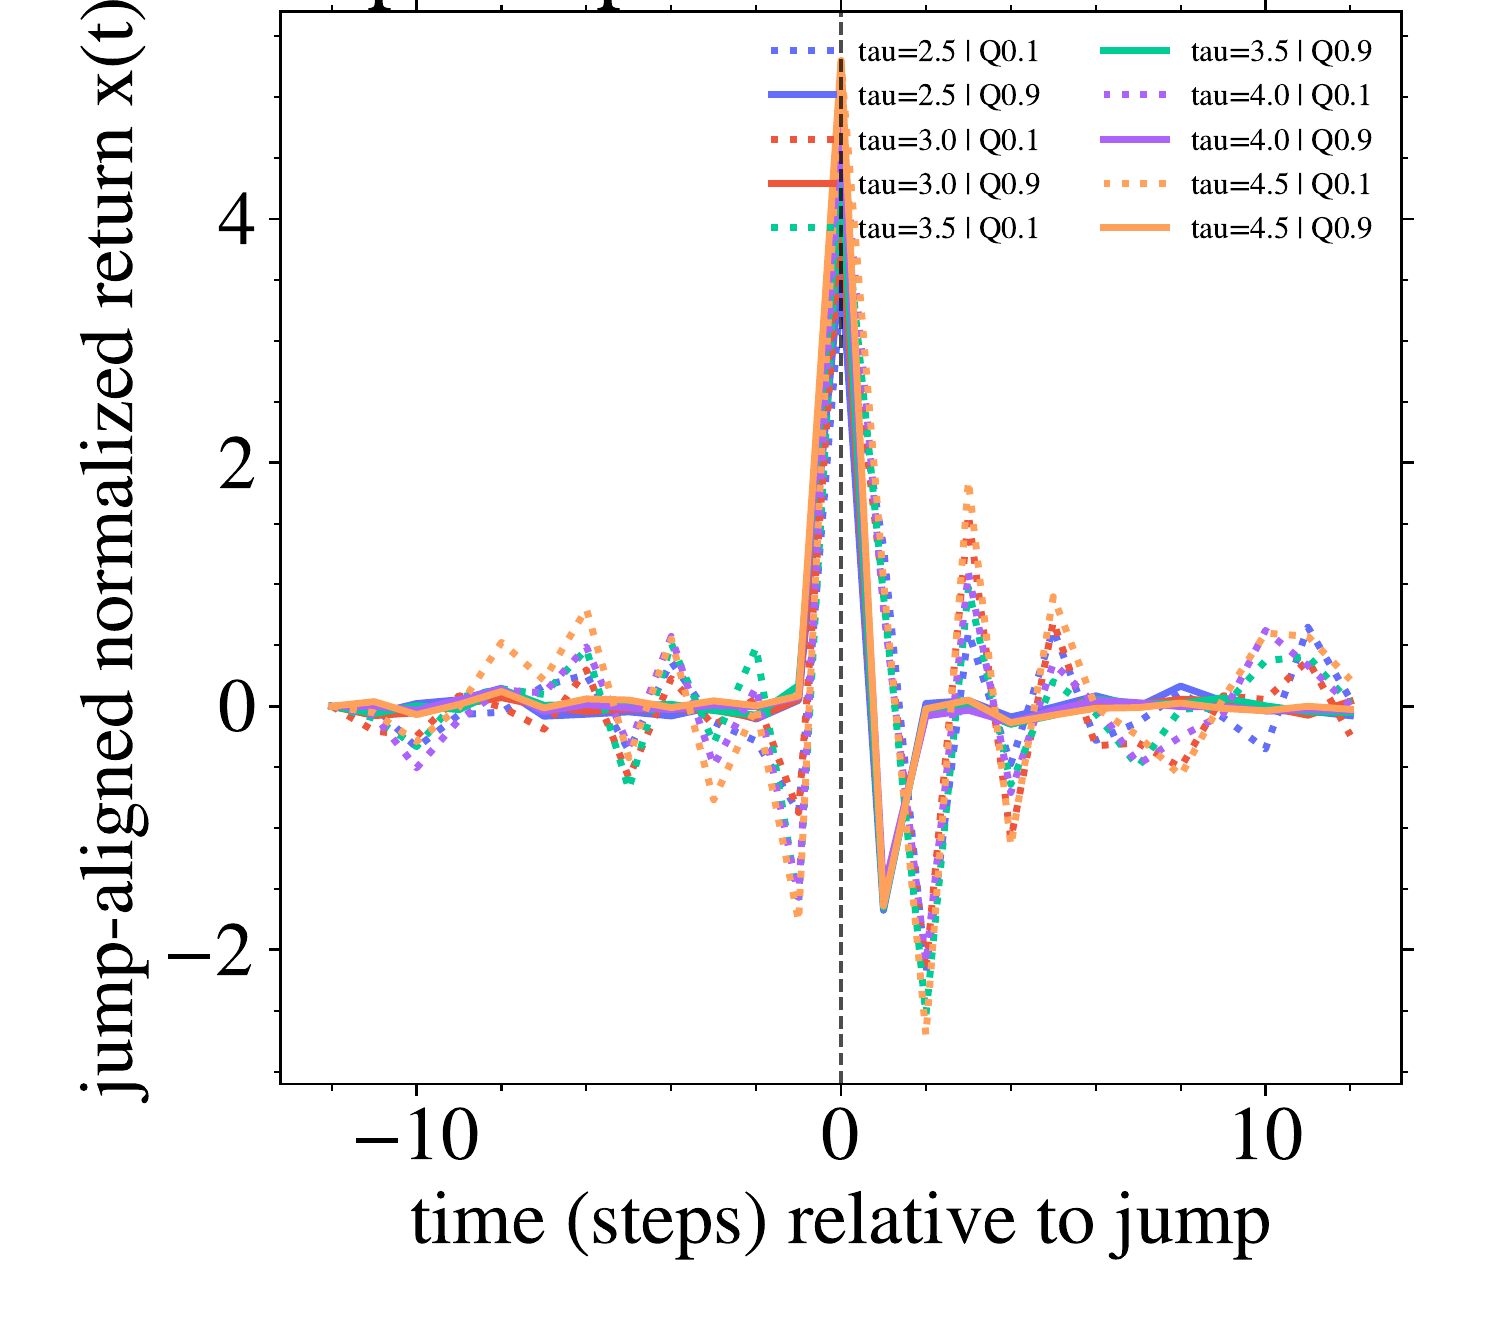
\includegraphics[width=\textwidth]{figures/2/overlay_D1_thresholds_5min_mpl.png}
    \caption{$D_1$ overlays.}
\end{subfigure}
\begin{subfigure}{0.32\textwidth}
    \centering
    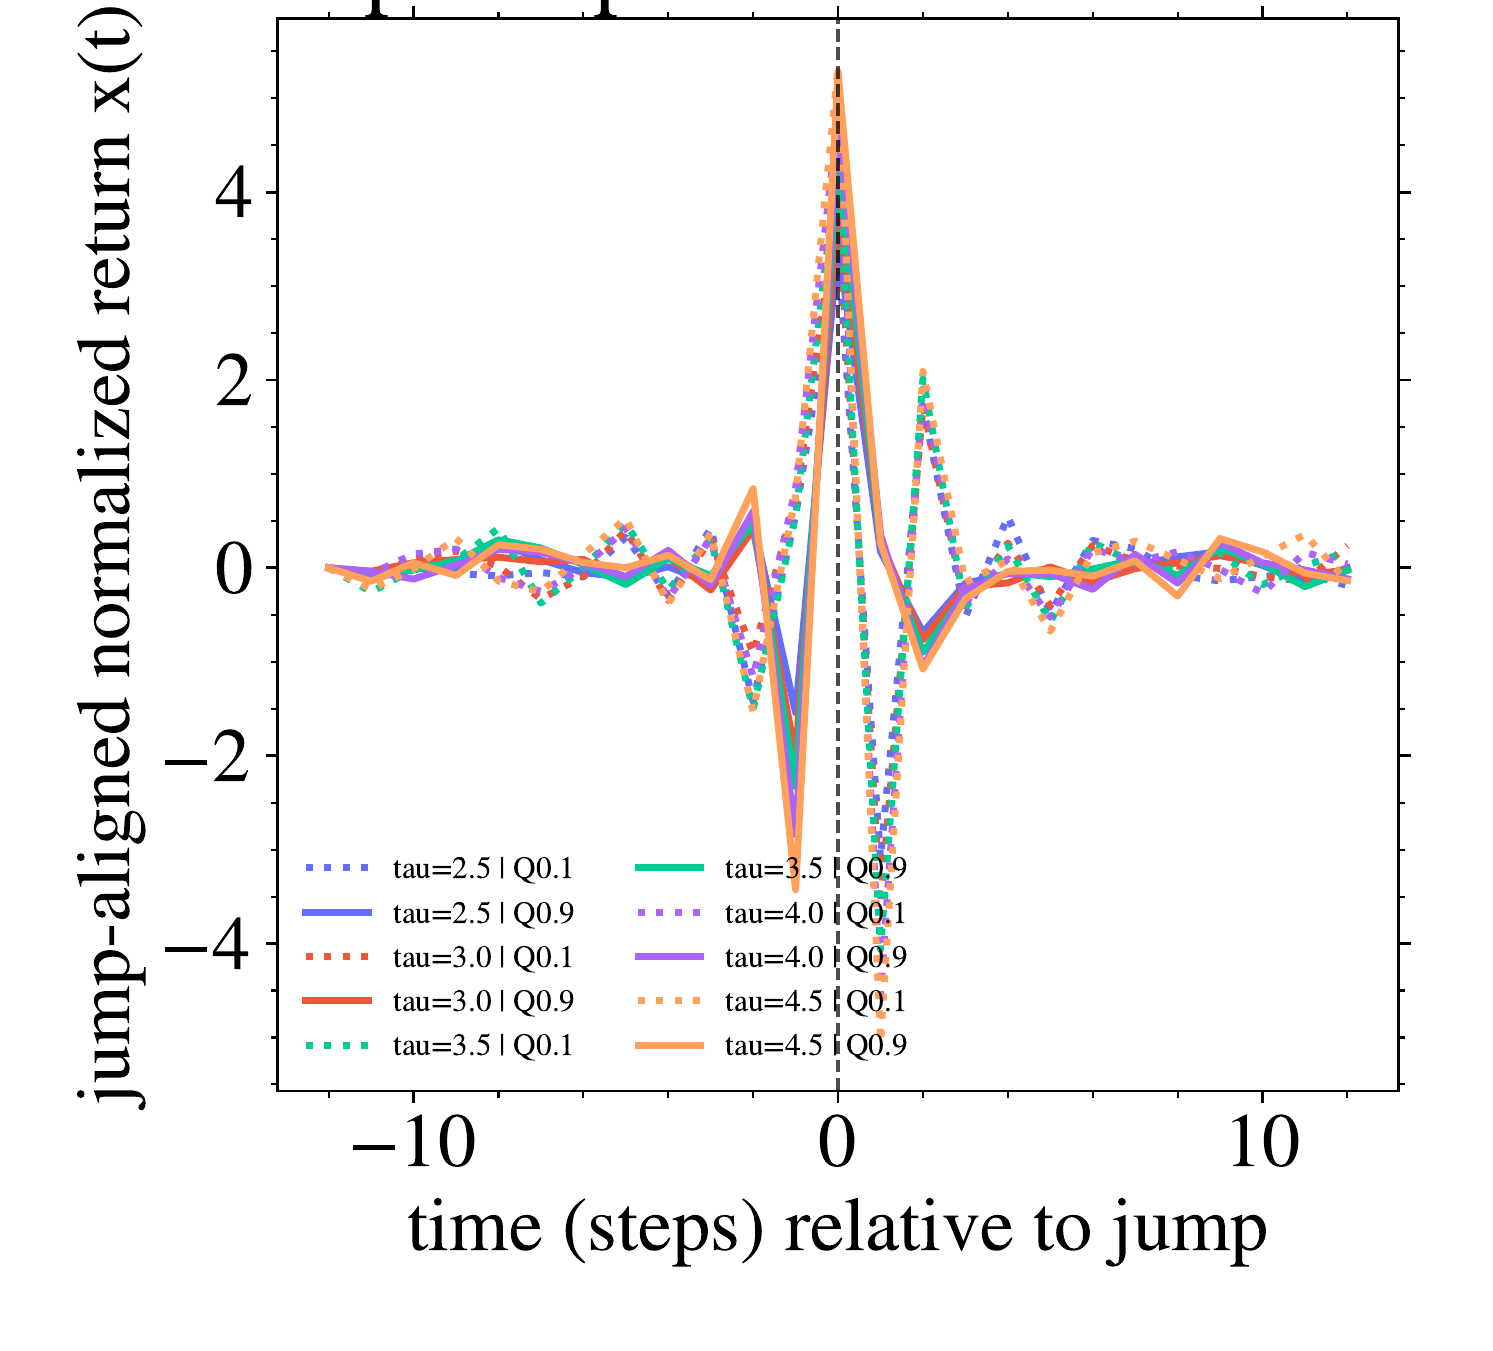
\includegraphics[width=\textwidth]{figures/2/overlay_D2_thresholds_5min_mpl.png}
    \caption{$D_2$ overlays.}
\end{subfigure}
\begin{subfigure}{0.32\textwidth}
    \centering
    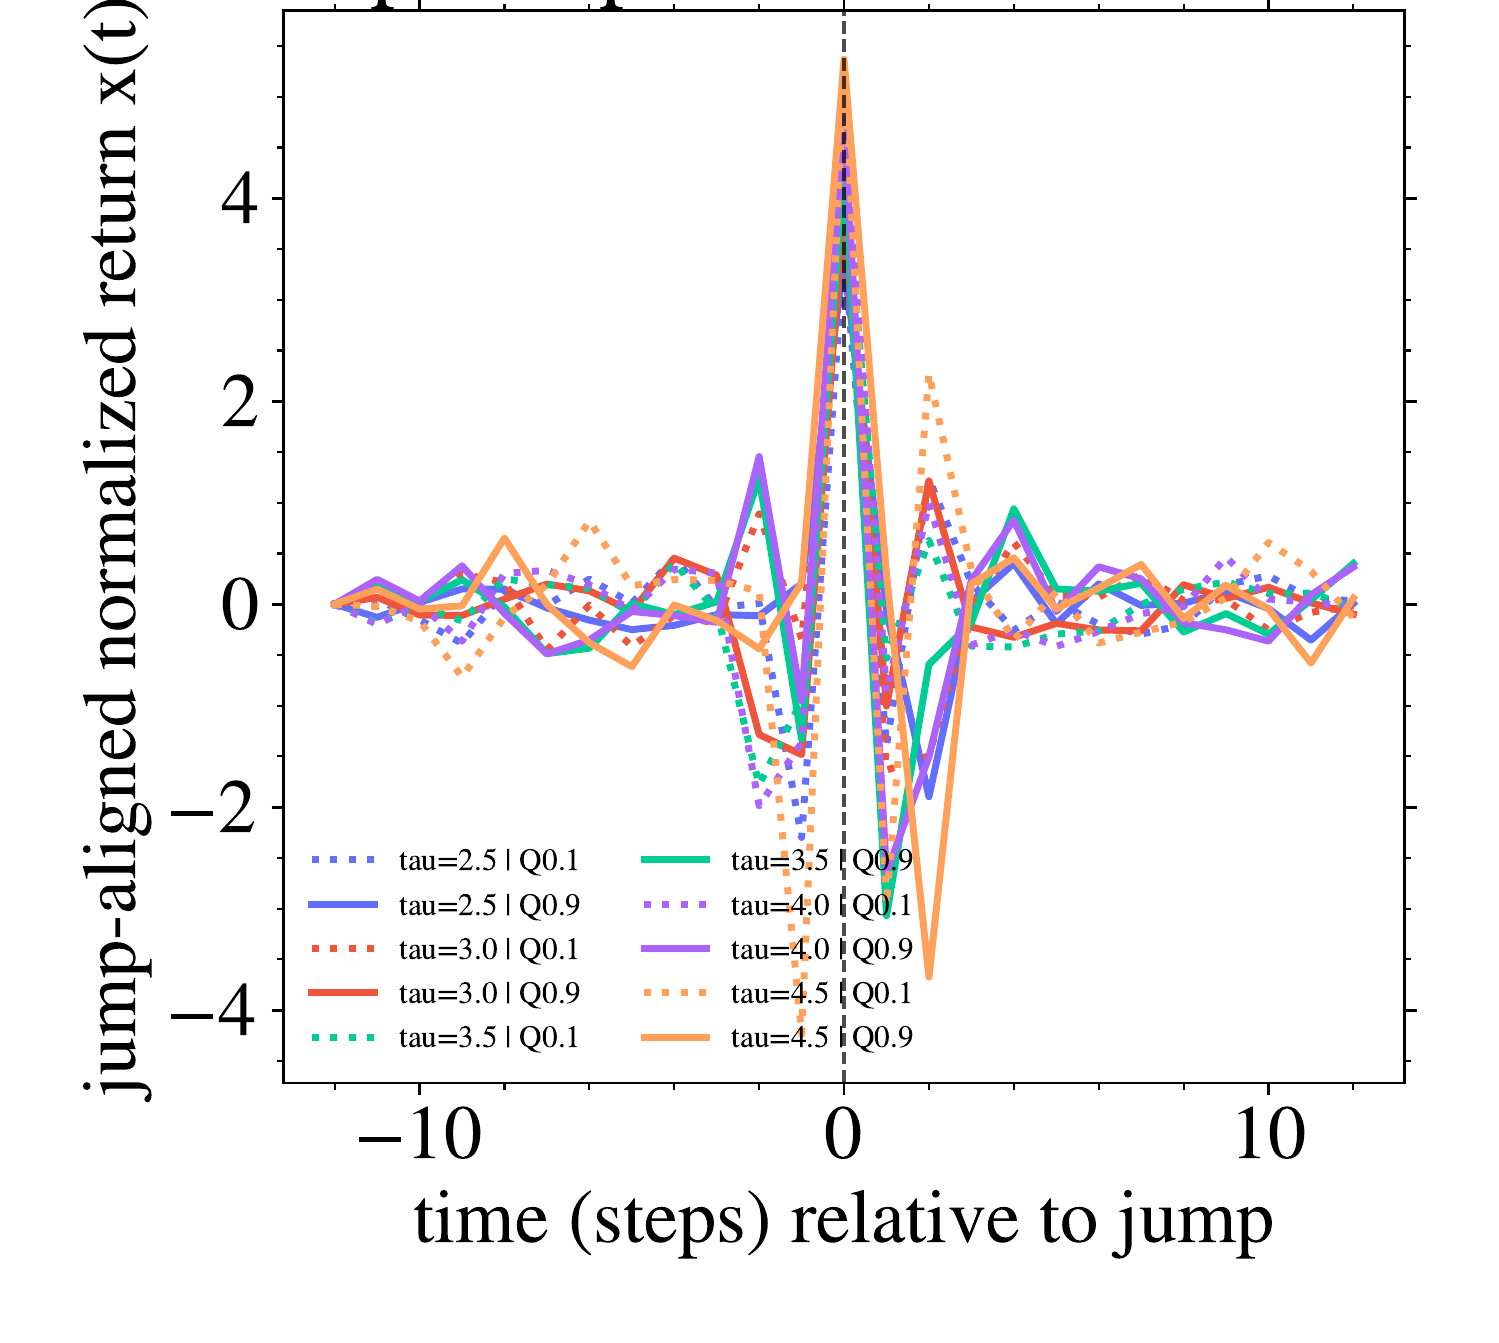
\includegraphics[width=\textwidth]{figures/2/overlay_D3_thresholds_5min_mpl.png}
    \caption{$D_3$ overlays.}
\end{subfigure}
\caption{Threshold sweep (5-min): average profiles along $D_1$, $D_2$, $D_3$ remain qualitatively stable across thresholds.}
\label{fig:threshold_sweep_5min}
\end{figure*}


\textbf{Kernel PCA method}: we tested the algorithm using both the RBF method and the linear method. The first one applies a kernel in an infinite-dimensional Hilbert space, while the latter is simply standard PCA on the 42-dimensional wavelet feature space.
The results in \ref{fig:kpca_projection} show that simple PCA performs as well as the more sophisticated RBF method, since it learns the same representation.\\

\textbf{Wavelet}: after testing the learned directions in \ref{fig:wavelet_coefficients_direction} and visualizing the top and lowest quantiles in each direction in \ref{fig:wavelet_quantiles}, we decided to keep the most common choice, the Morlet wavelet with bandwidth 1.5 and center frequency 1.0, since all wavelets give similar results but this one produces smoother shapes.\\

\textbf{J parameter}: by increasing the parameter $J$, we increase the dimension of the wavelet feature space. Surprisingly, as shown in \ref{fig:J_values_quantiles}, increasing it up to $J=9$ does not better capture the properties we are interested in. For instance, the second direction captures mean reversion more clearly with $J=3$, which should theoretically be the worst-performing setting. We conclude that the learned directions are not very stable with respect to hyperparameter changes, and that each configuration must be empirically evaluated. 


\begin{figure}[htbp]
    \centering
    \begin{subfigure}[b]{0.32\textwidth}
        \centering
        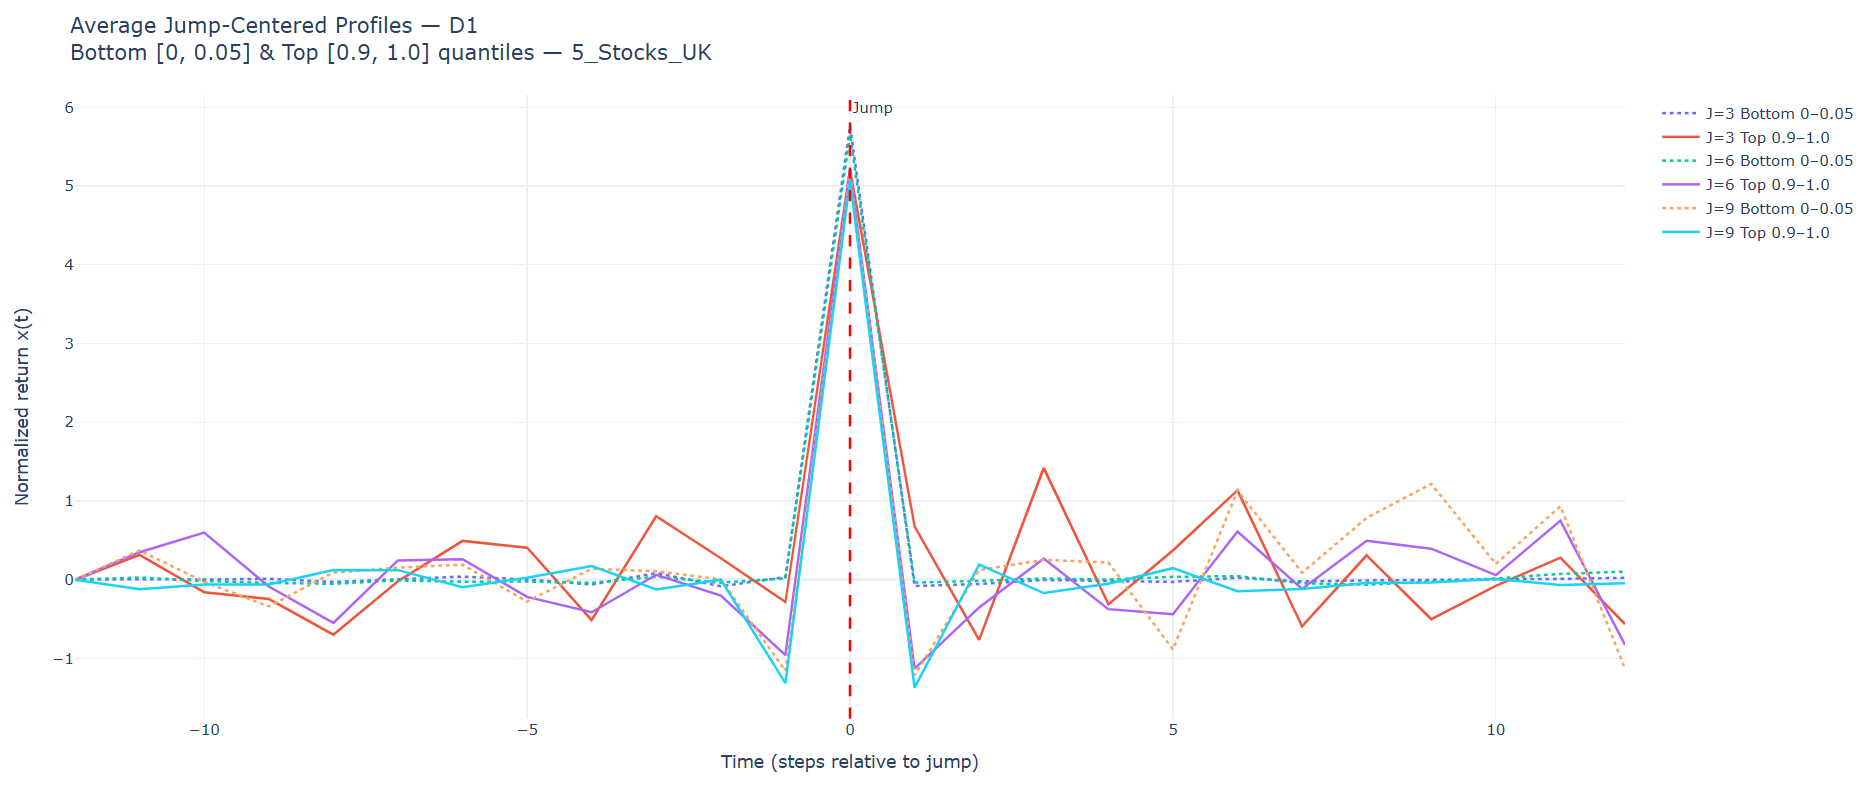
\includegraphics[width=\textwidth]{D1_J_values.png}
        \caption{First PCA direction}
    \end{subfigure}
    \hfill
    \begin{subfigure}[b]{0.32\textwidth}
        \centering
        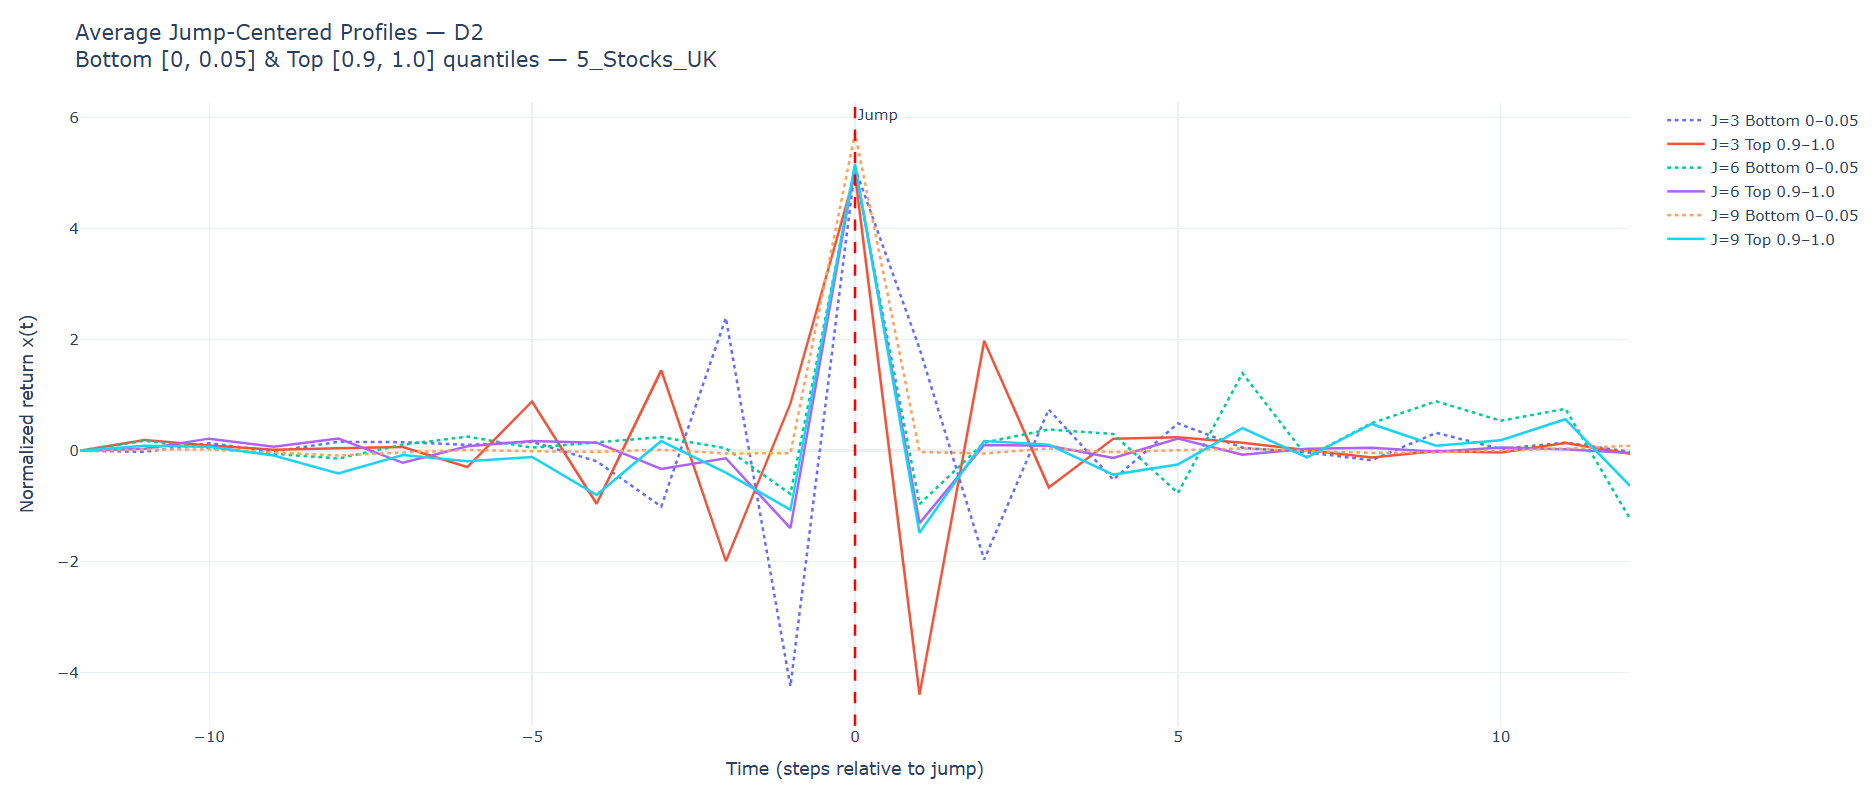
\includegraphics[width=\textwidth]{D2_J_values.png}
        \caption{Second PCA direction}
    \end{subfigure}
    \hfill
    \begin{subfigure}[b]{0.32\textwidth}
        \centering
        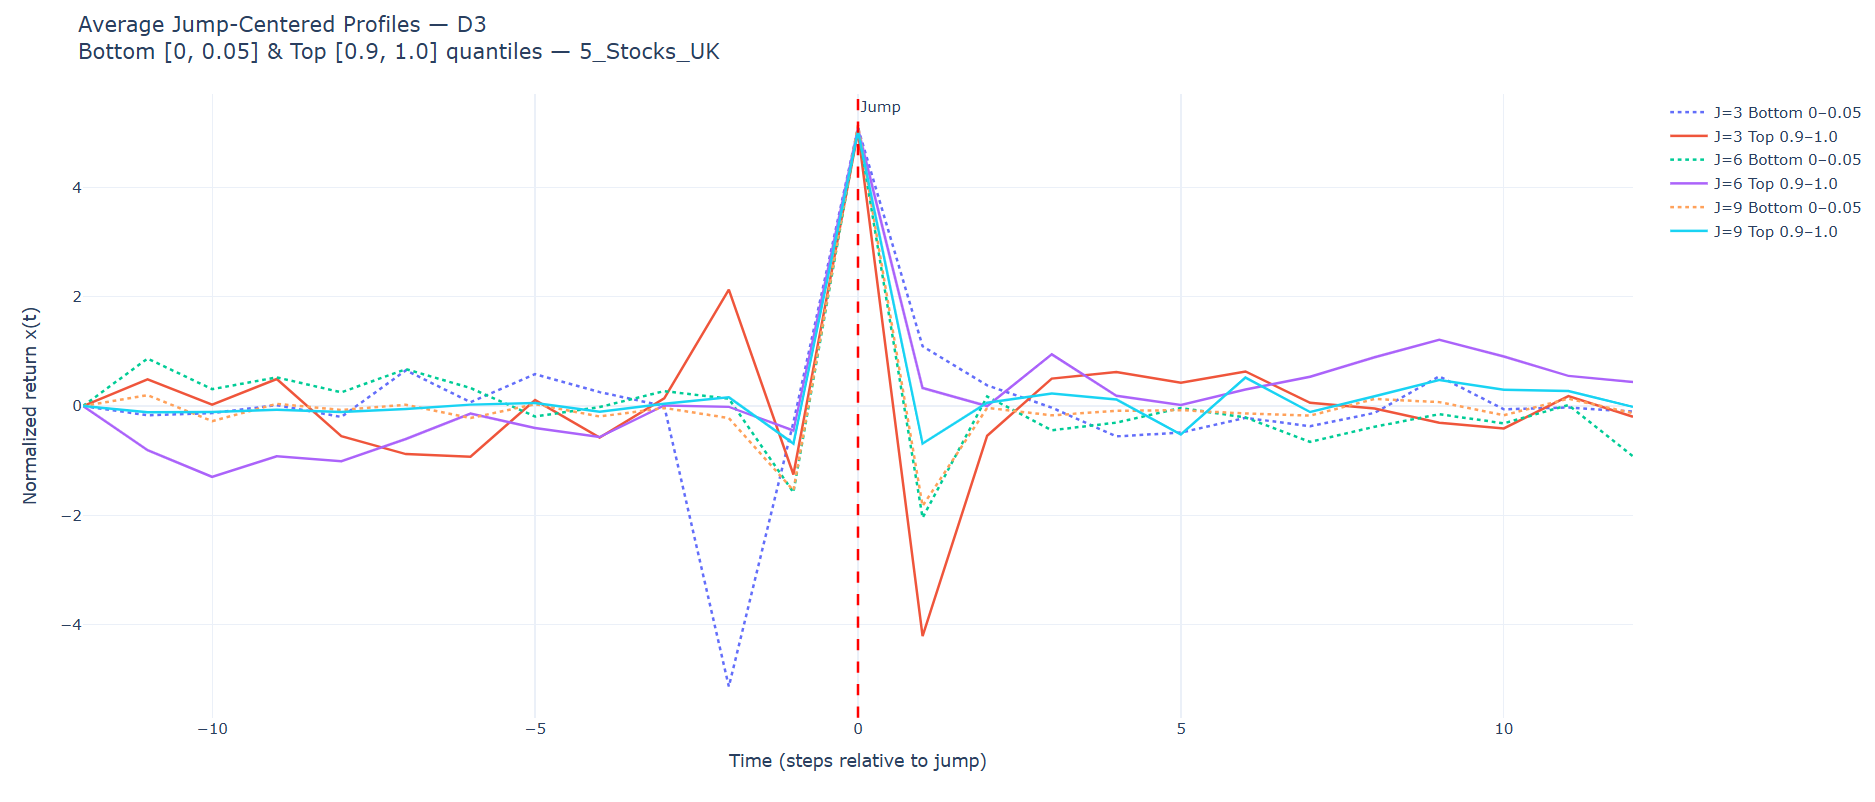
\includegraphics[width=\textwidth]{D3_J_values.png}
        \caption{Third PCA direction}
    \end{subfigure}
    \caption{Visulization of first and last quantiles jumps on UK stock data for different values of $J$.}
    \label{fig:J_values_quantiles}
\end{figure}

%\textbf{Threshold hyperparameter}: The jump is detected in the paper by setting $|x(t)|>4$, but we can of course modify this threshold. The larger the value, the less jumps we will detect in a dataset and the more accentuated jumps will be. As shown in 
\textbf{Different countries}: since the data come from several countries, we can test whether the algorithm consistently learns the same features. As shown in \ref{fig:different_countries}, the learned directions are quite similar across countries. The paper states that the first direction is a linear combination of the 15 imaginary second-order wavelet coefficients. While this interpretation is conceptually appealing, as it relates to time asymmetry, our results suggest that this direction is not purely that feature. % Although it correlates with time asymmetry, other properties appear to be mixed in, as the algorithm sometimes favors well-defined peaks with nearly constant values on both sides.


\begin{figure}[htbp]
    \centering
    \begin{subfigure}[b]{0.32\textwidth}
        \centering
        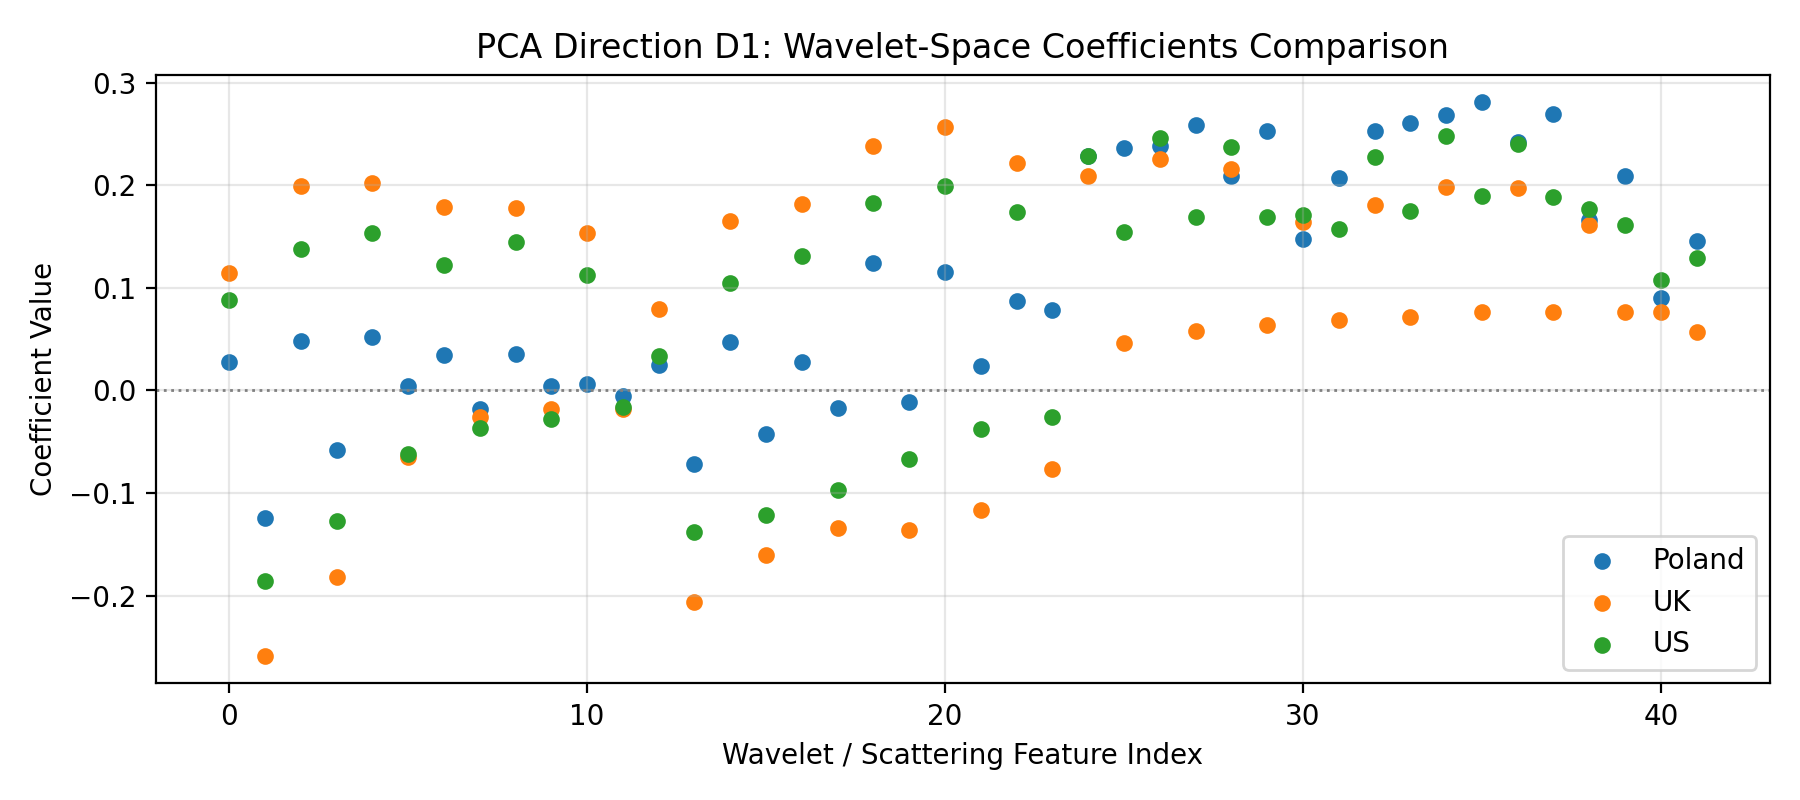
\includegraphics[width=\textwidth]{D1_components_comparison_scatter.png}
        \caption{First PCA direction}
    \end{subfigure}
    \hfill
    \begin{subfigure}[b]{0.32\textwidth}
        \centering
        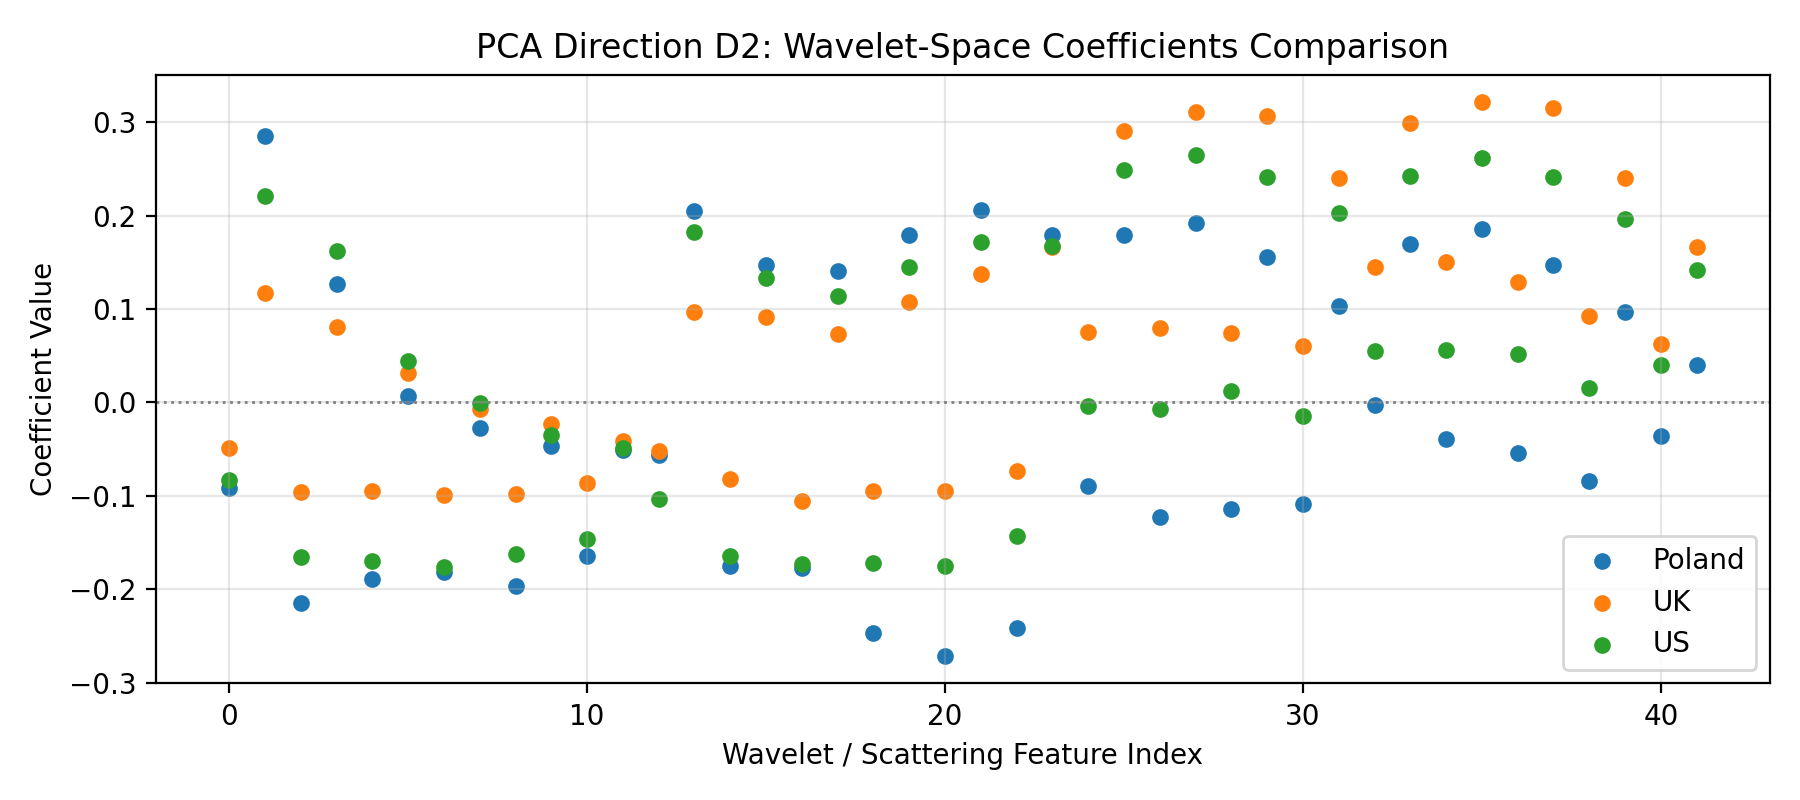
\includegraphics[width=\textwidth]{D2_components_comparison_scatter.png}
        \caption{Second PCA direction}
    \end{subfigure}
    \hfill
    \begin{subfigure}[b]{0.32\textwidth}
        \centering
        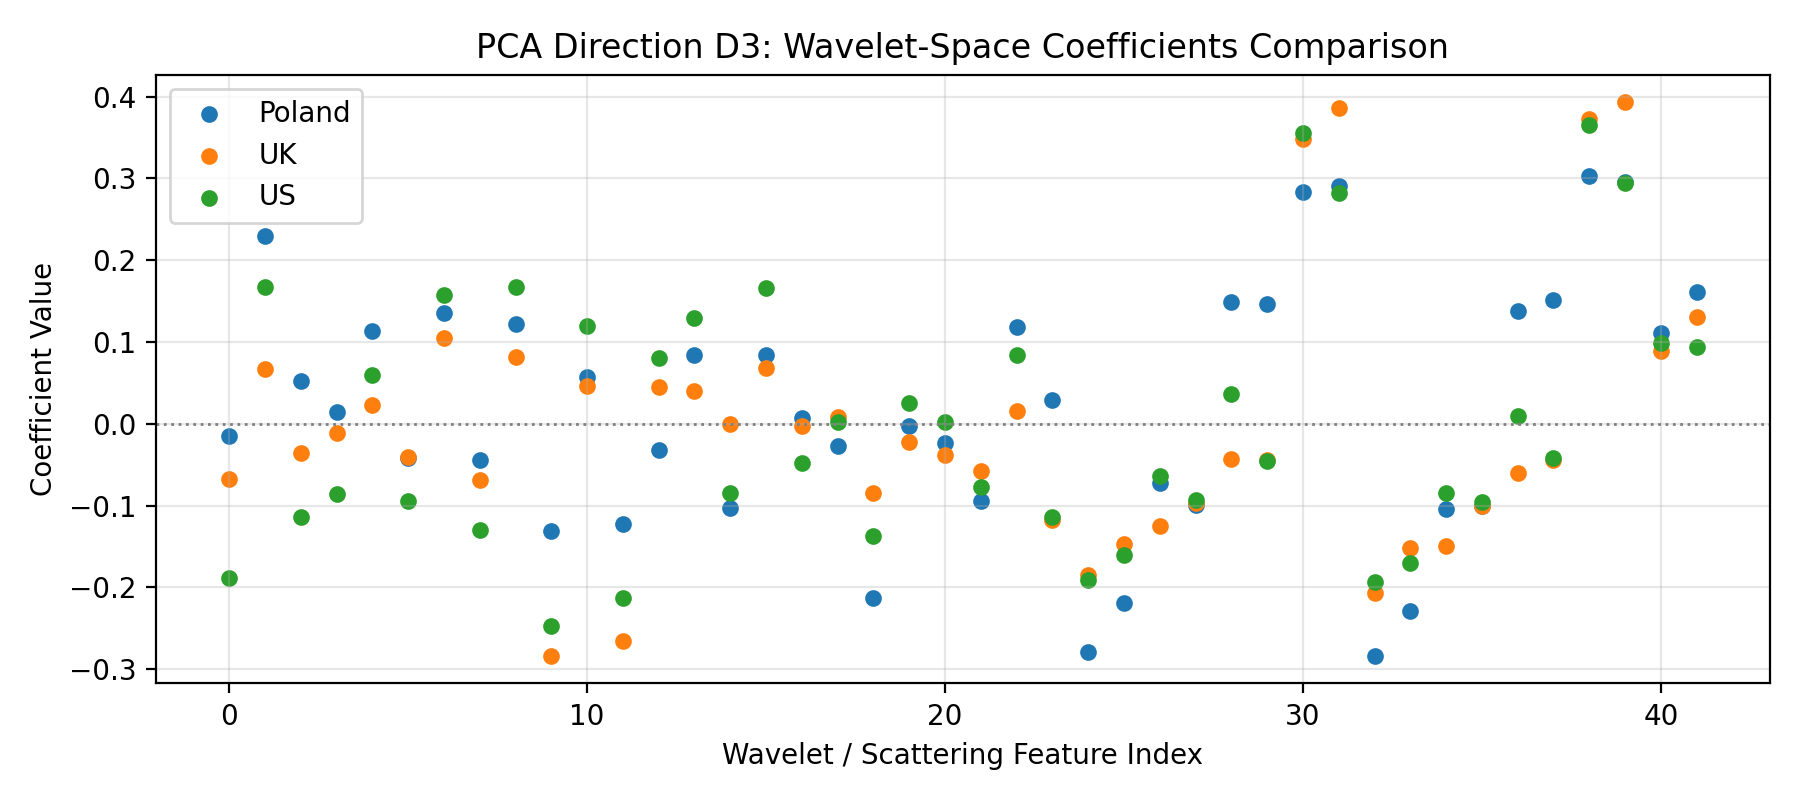
\includegraphics[width=\textwidth]{D3_components_comparison_scatter.png}
        \caption{Third PCA direction}
    \end{subfigure}
    \caption{Learned directions for the first 3 PCA direction from data of 3 different countries: Poland, UK and US.}
    \label{fig:different_countries}
\end{figure}

\subsection{Relation between learned features and hand crafted features}

Here we address the following question: are the handcrafted features relevant to the features learned via PCA on wavelet coefficients? This question is central to the original paper, which claims that well-established financial features can be recovered in an unsupervised manner. We examine the correlations between handcrafted and learned features, as shown in \ref{fig:PCA_hand_craft}. The first PCA direction is the best explained by its corresponding handcrafted feature, exhibiting a strong positive correlation and a non-negligible $R^2$ value. The third direction also correlates with the trend feature (correlation of 0.32), while the second direction clearly differs from mean reversion. This suggests that unsupervised feature extraction does not necessarily recover the expected financial descriptors. It may also indicate that other latent properties of the data are relevant, that alternative feature representations could be informative, or that the difference arises from using 5-minute data instead of 1-minute data.


\begin{figure}[htbp]
    \centering
    \begin{subfigure}[b]{0.32\textwidth}
        \centering
        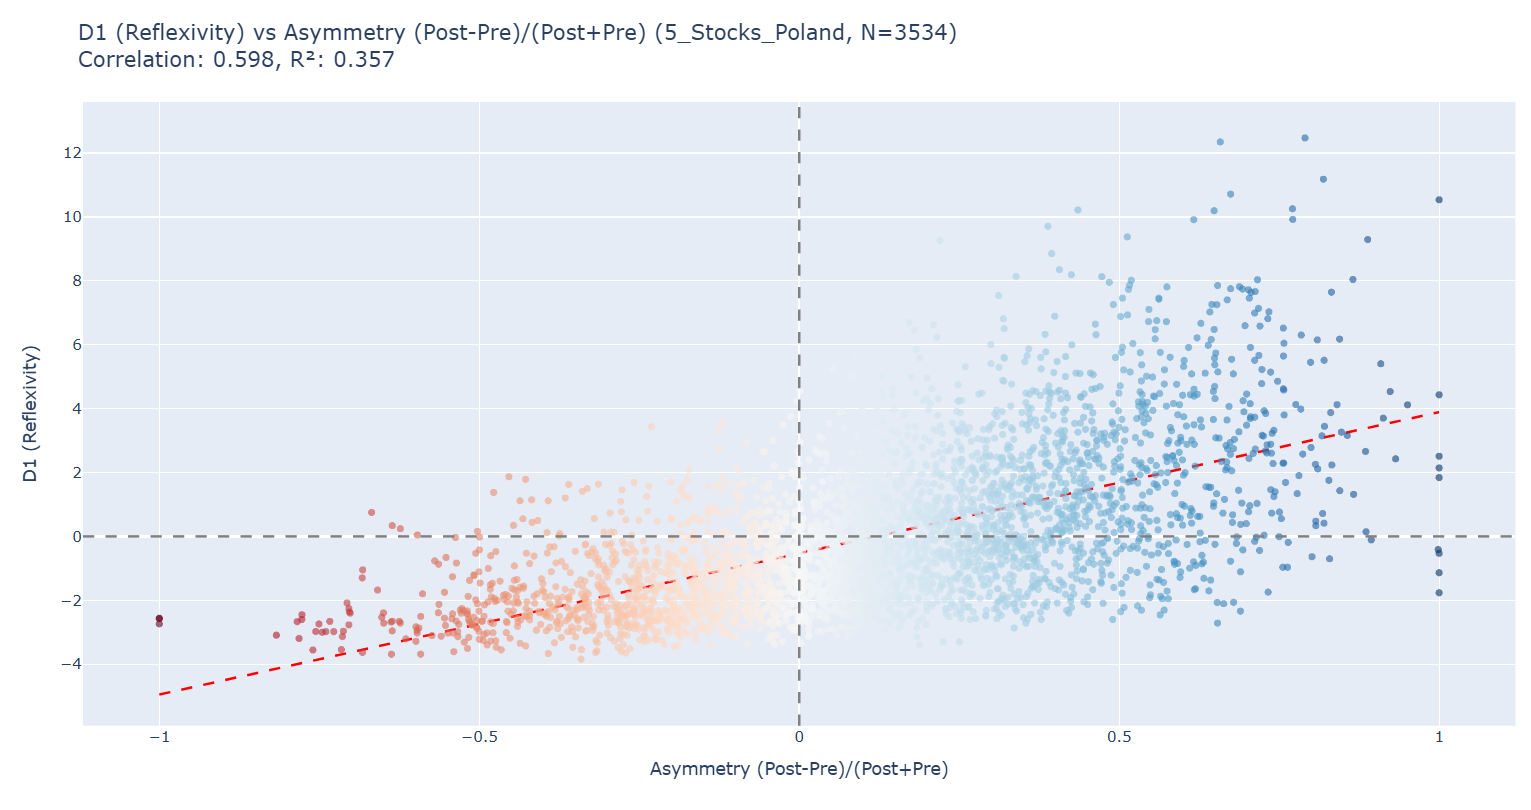
\includegraphics[width=\textwidth]{D1_asymmetry.png}
        \caption{First PCA direction vs Asymmetry}
    \end{subfigure}
    \hfill
    \begin{subfigure}[b]{0.32\textwidth}
        \centering
        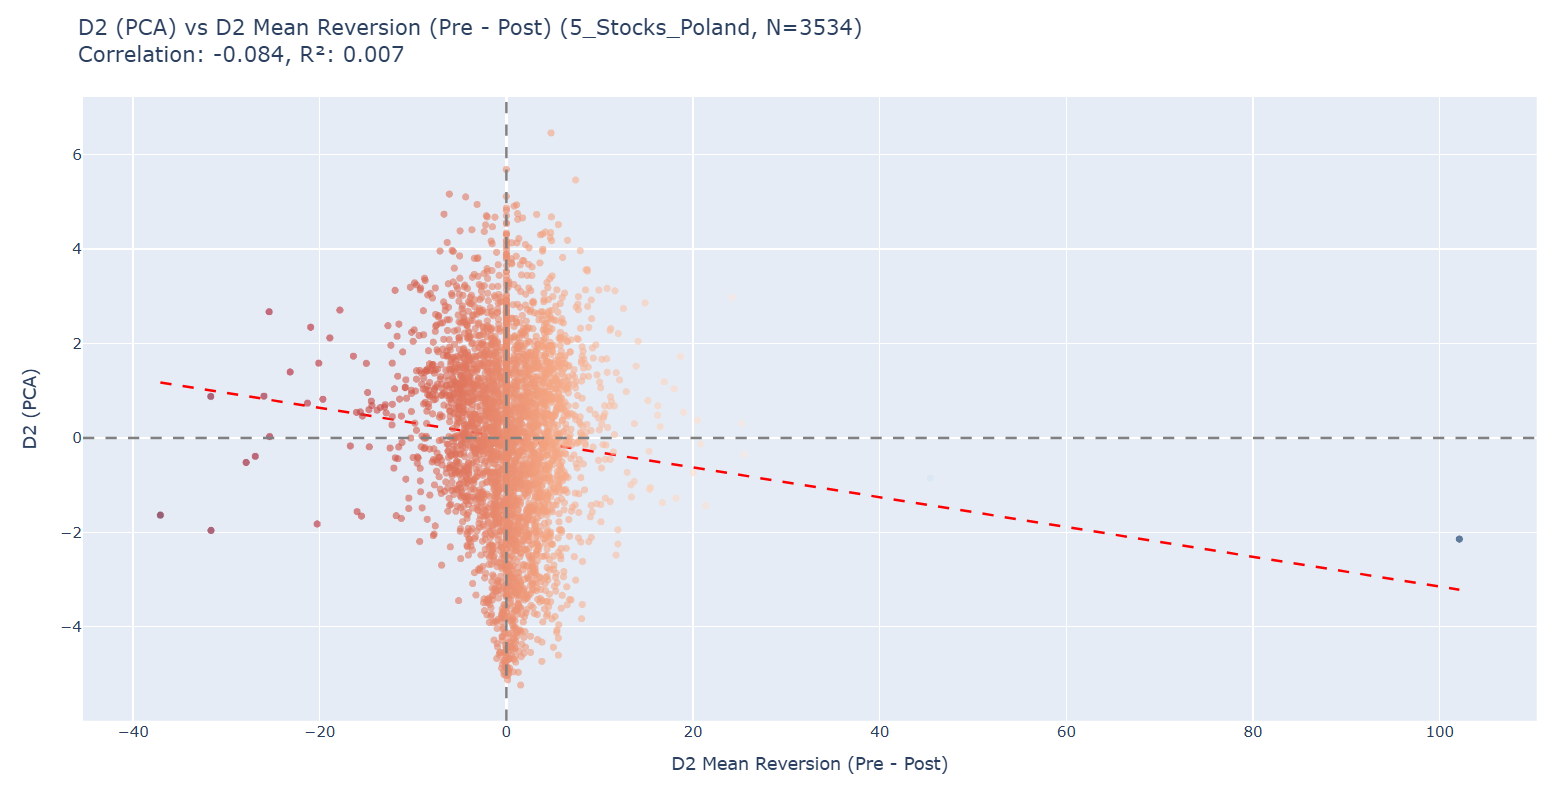
\includegraphics[width=\textwidth]{D2_mean_reversion.png}
        \caption{Second PCA direction vs Mean reversion}
    \end{subfigure}
    \hfill
    \begin{subfigure}[b]{0.32\textwidth}
        \centering
        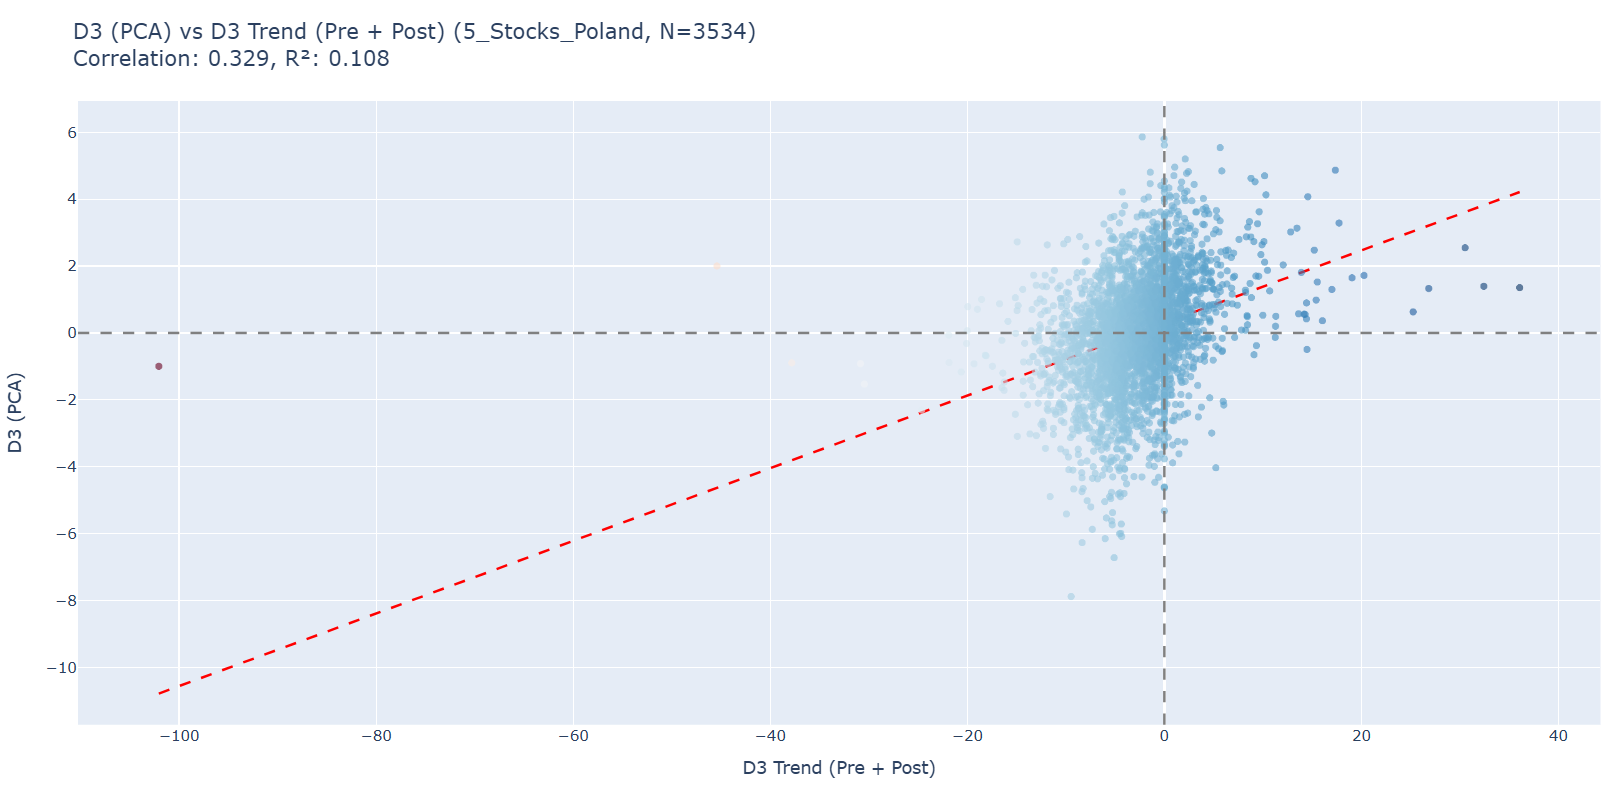
\includegraphics[width=\textwidth]{D3_trend.png}
        \caption{Third PCA direction vs Trend}
    \end{subfigure}
    \caption{Correlation between learned PCA directions and hand crafted features. Experiment done with 5 minutes Poland stock}
    \label{fig:PCA_hand_craft}
\end{figure}



% \paragraph{Conclusion.}
% Our reproduction confirms that wavelet-based embeddings recover interpretable jump classes, with $D_1$ measuring volatility time-asymmetry and complementary mean-reversion/trend directions emerging from local signed profiles. On our open-data setting, Scattering Spectra features do not materially change the main reflexivity direction.

% \begin{thebibliography}{9}
% \bibitem{aubrun_ridingwavelets}
% C.~Aubrun, R.~Morel, M.~Benzaquen, and J.-P.~Bouchaud.
% \newblock Riding wavelets: A method to discover new classes of price jumps.
% \newblock (preprint / manuscript version in \texttt{refs/texsources/ridingwavelets}).

% \bibitem{bruna_mallat}
% J.~Bruna and S.~Mallat.
% \newblock Invariant scattering convolution networks.
% \newblock \emph{IEEE Transactions on Pattern Analysis and Machine Intelligence}, 35(8):1872--1886, 2013.

% \bibitem{morel_scatteringspectra}
% R.~Morel et al.
% \newblock Scattering spectra for scale-invariant time series analysis.
% \newblock (see references in the original paper).
% \end{thebibliography}

\bibliographystyle{plain}   % or alpha, abbrv, unsrt, etc.
\bibliography{references}


\section*{Appendix}

\begin{figure}[htbp]
    \centering
    \begin{subfigure}[b]{0.32\textwidth}
        \centering
        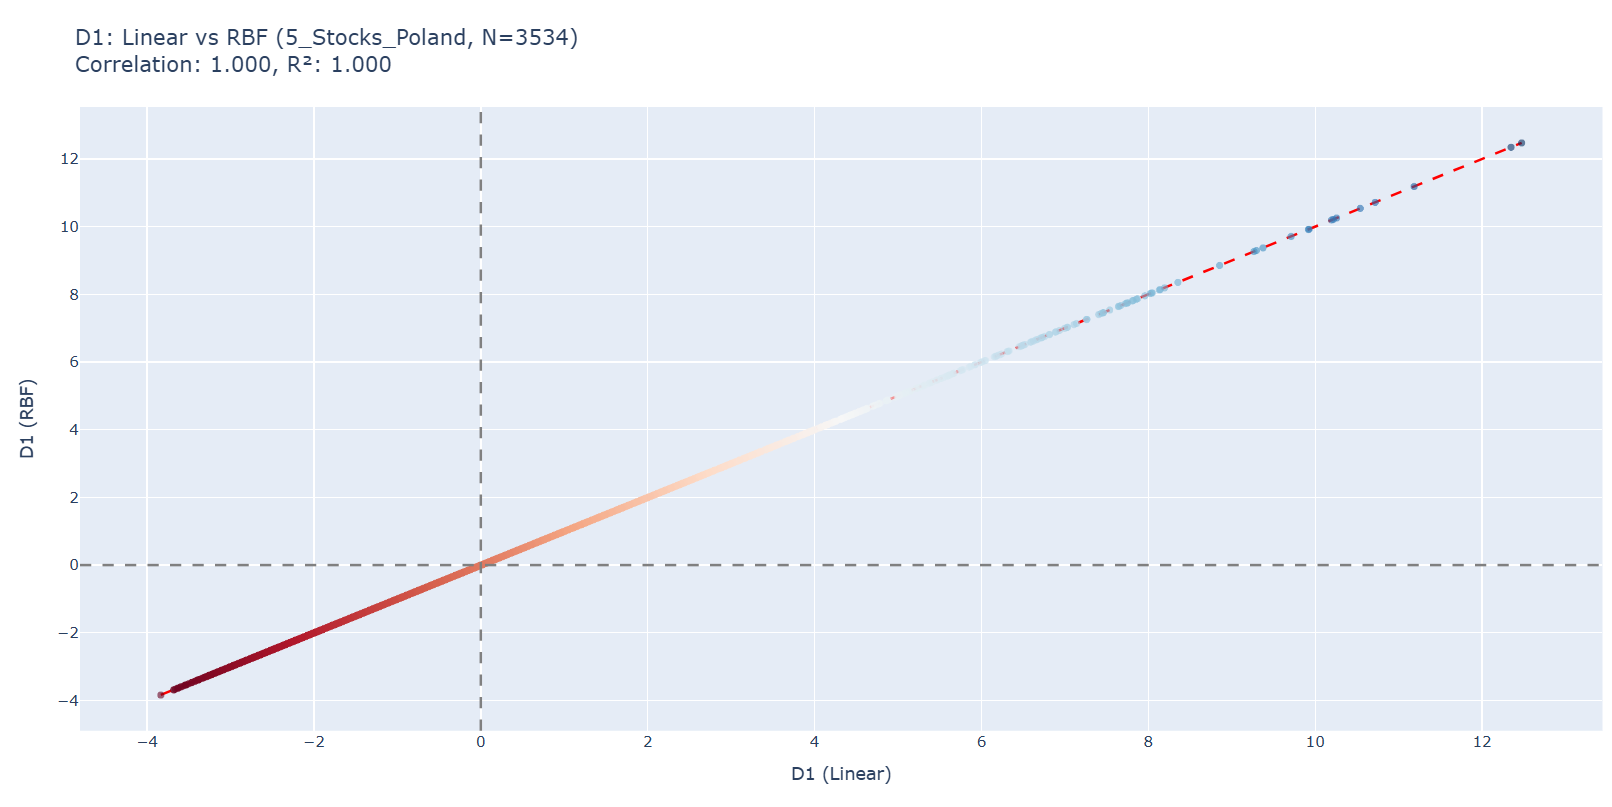
\includegraphics[width=\textwidth]{D1_rbf_linear.png}
        \caption{First KPCA direction}
        \label{fig:D1}
    \end{subfigure}
    \hfill
    \begin{subfigure}[b]{0.32\textwidth}
        \centering
        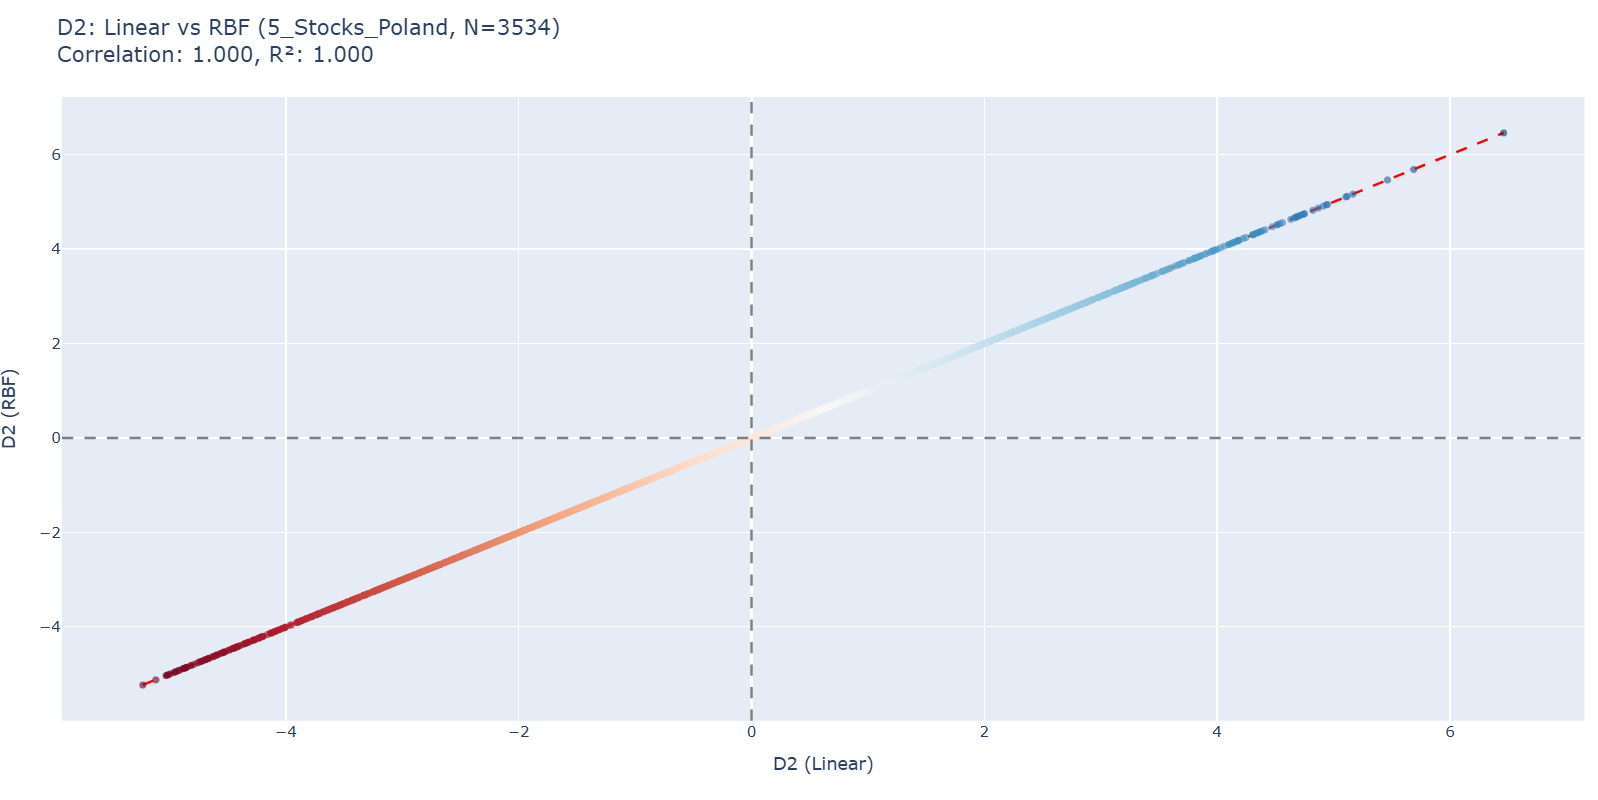
\includegraphics[width=\textwidth]{D2_rbf_linear.png}
        \caption{Second KPCA direction}
        \label{fig:D2}
    \end{subfigure}
    \hfill
    \begin{subfigure}[b]{0.32\textwidth}
        \centering
        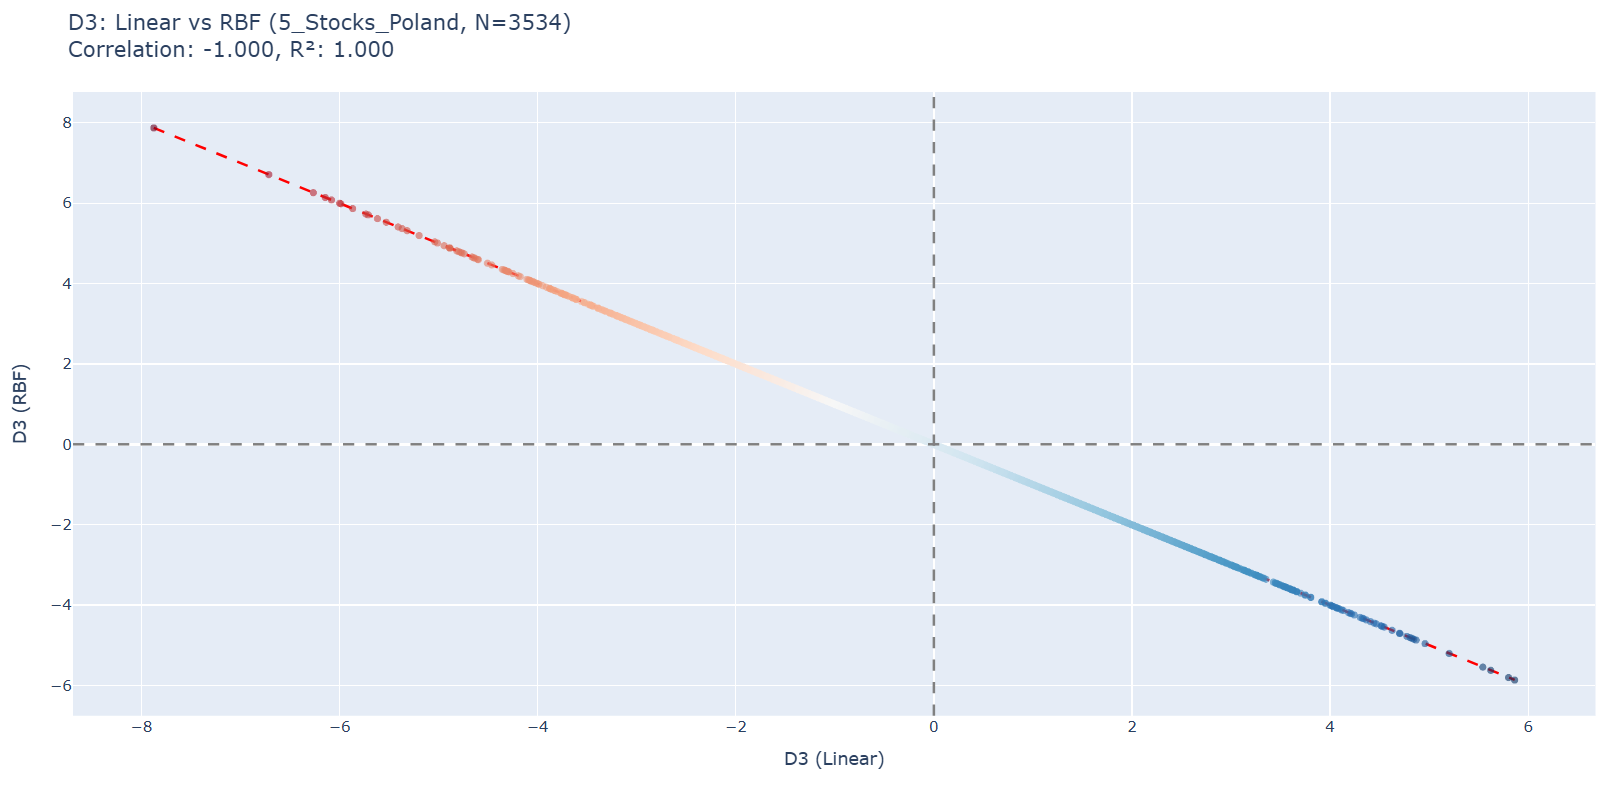
\includegraphics[width=\textwidth]{D3_rbf_linear.png}
        \caption{Third KPCA direction}
        \label{fig:D3}
    \end{subfigure}
    \caption{Projected jumps from Polish stocks onto the first three KPCA directions. Shows correlation between the RBF and linear methods.}
    \label{fig:kpca_projection}
\end{figure}

\begin{figure}[htbp]
    \centering
    \begin{subfigure}[b]{0.3\textwidth}
        \centering
        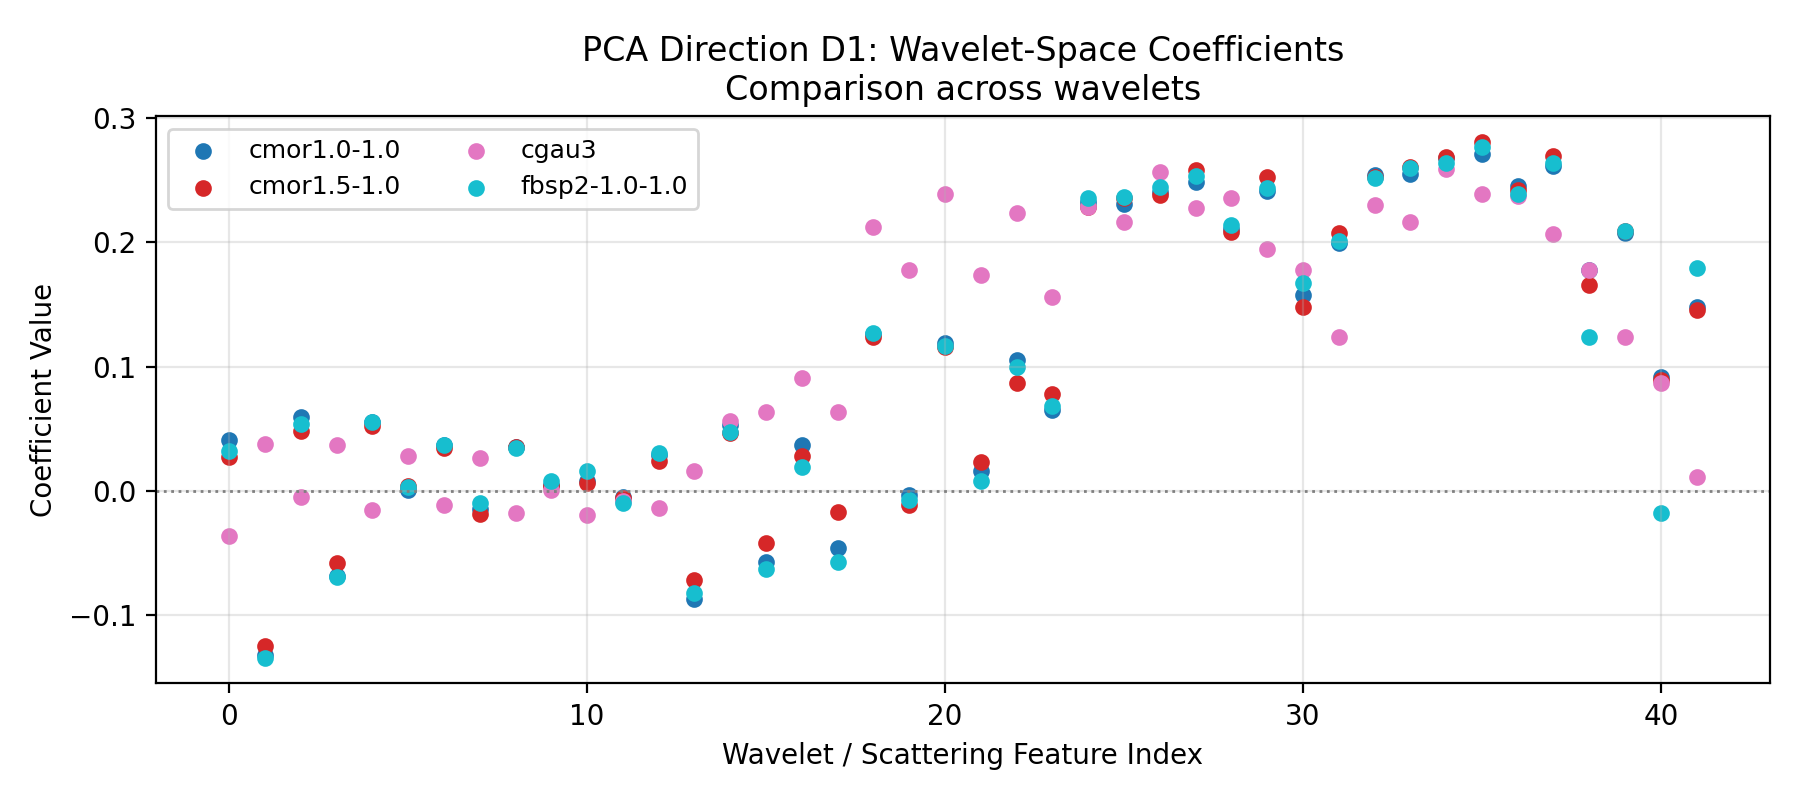
\includegraphics[width=\textwidth]{D1_components_wavelets_scatter.png}
        \caption{First KPCA direction}
    \end{subfigure}
    \hfill
    \begin{subfigure}[b]{0.3\textwidth}
        \centering
        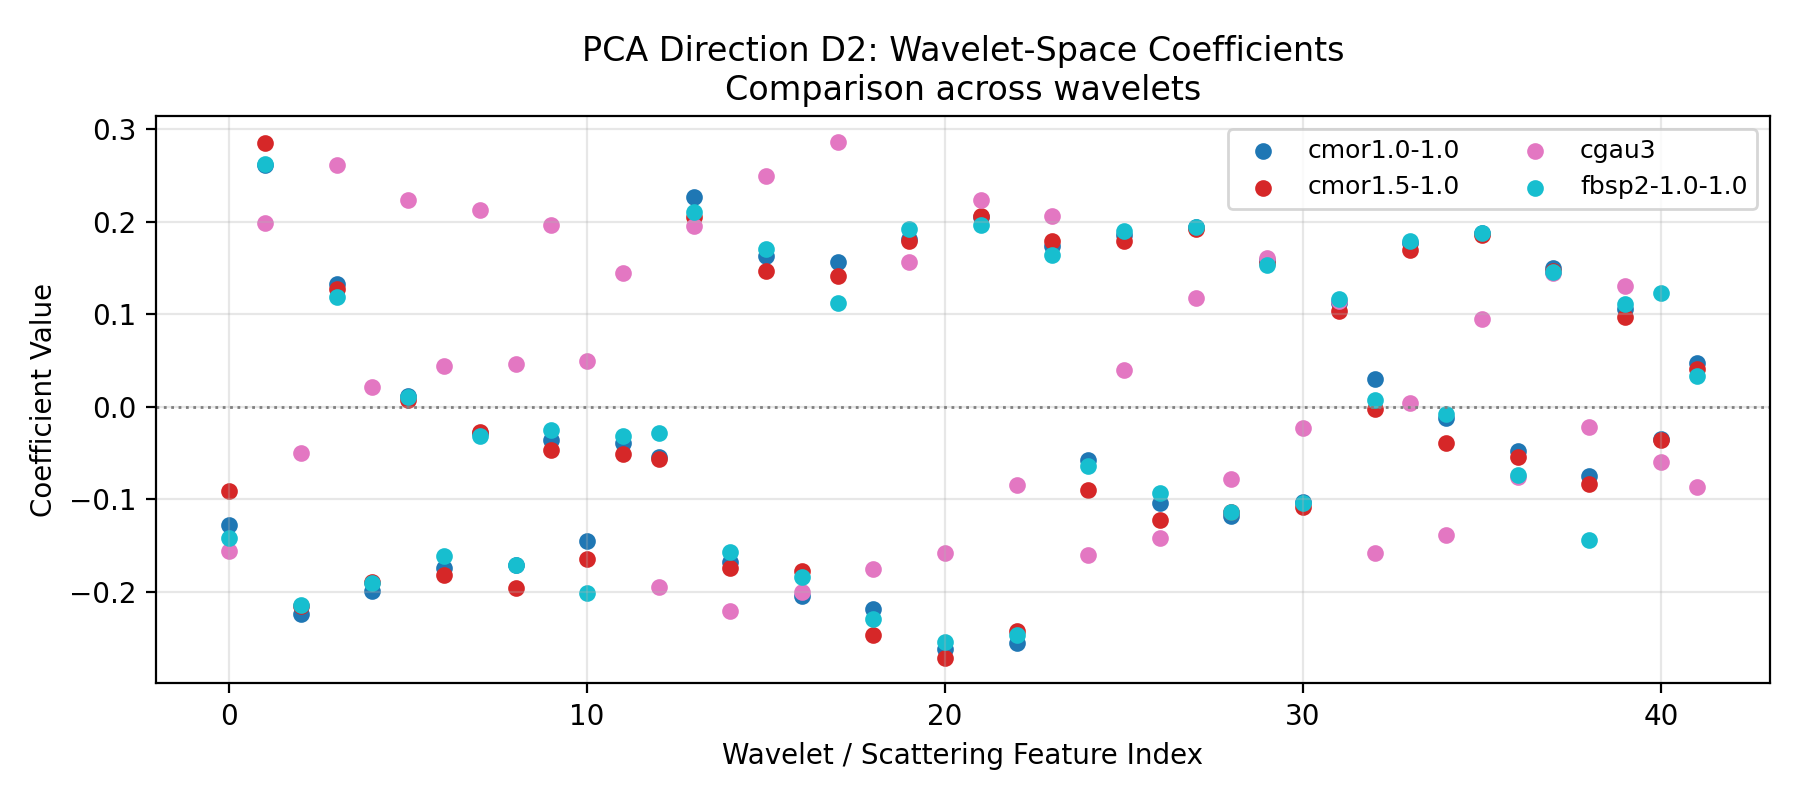
\includegraphics[width=\textwidth]{D2_components_wavelets_scatter.png}
        \caption{Second KPCA direction}
    \end{subfigure}
    \hfill
    \begin{subfigure}[b]{0.3\textwidth}
        \centering
        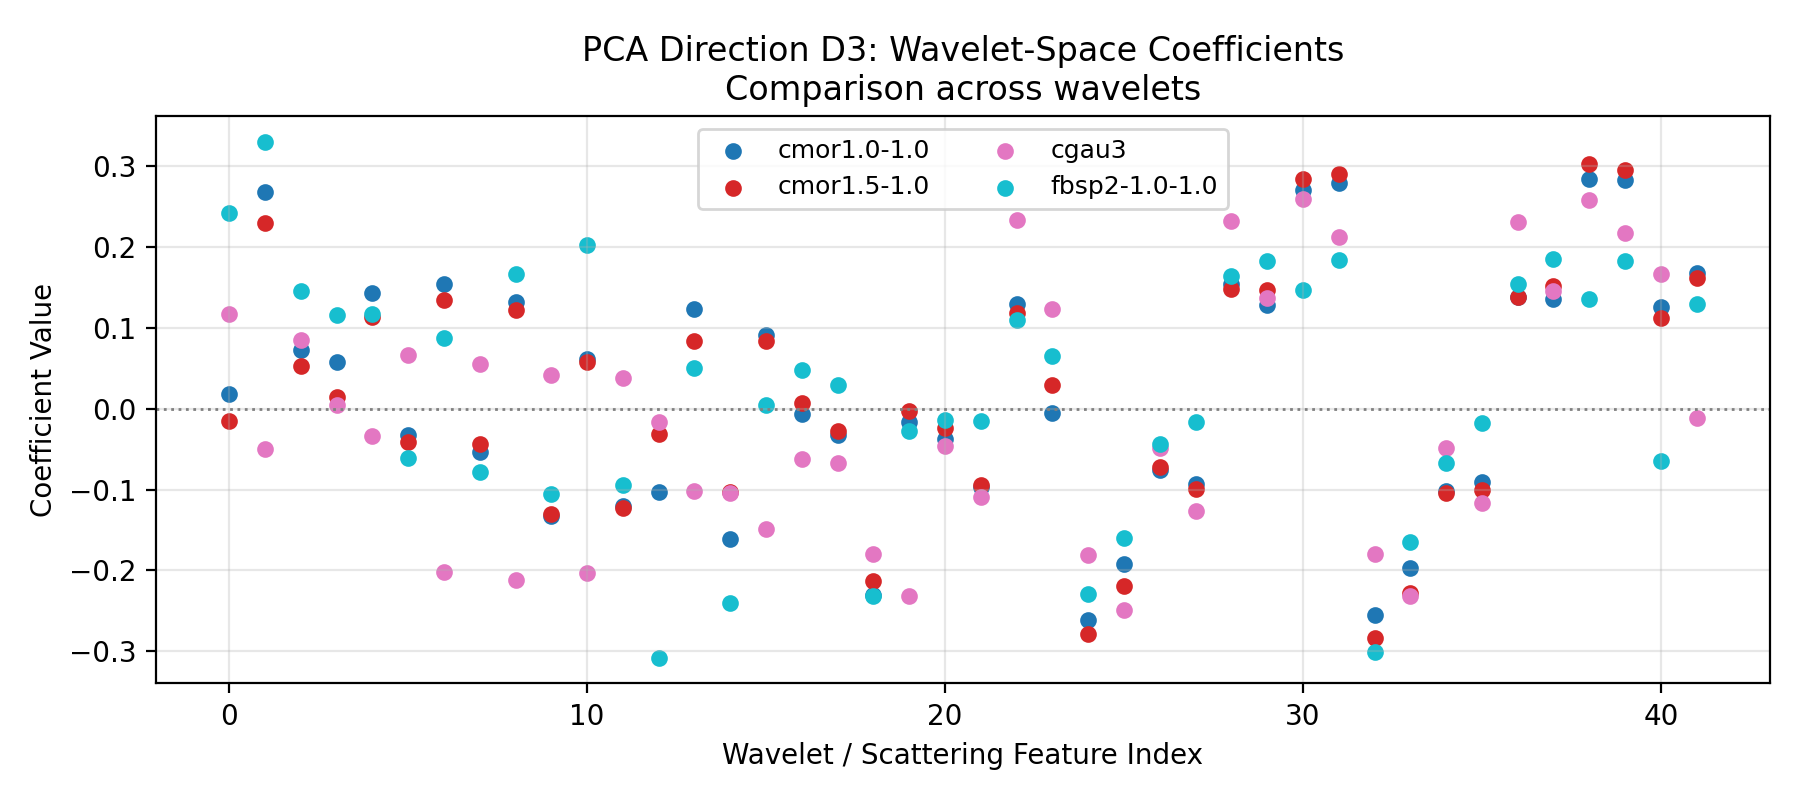
\includegraphics[width=\textwidth]{D3_components_wavelets_scatter.png}
        \caption{Third KPCA direction}
    \end{subfigure}
    \caption{Learned PCA directions in wavelet space on Poland stock data for wavelets: 2 complex Morlet (cmor), 1 complex Guassian (cgau) and a frequency B spline (fbsp). Each graph represents the direction coefficients for each of the 42 wavelet components.}
    \label{fig:wavelet_coefficients_direction}
\end{figure}

\begin{figure}[htbp]
    \centering
    \begin{subfigure}[b]{0.32\textwidth}
        \centering
        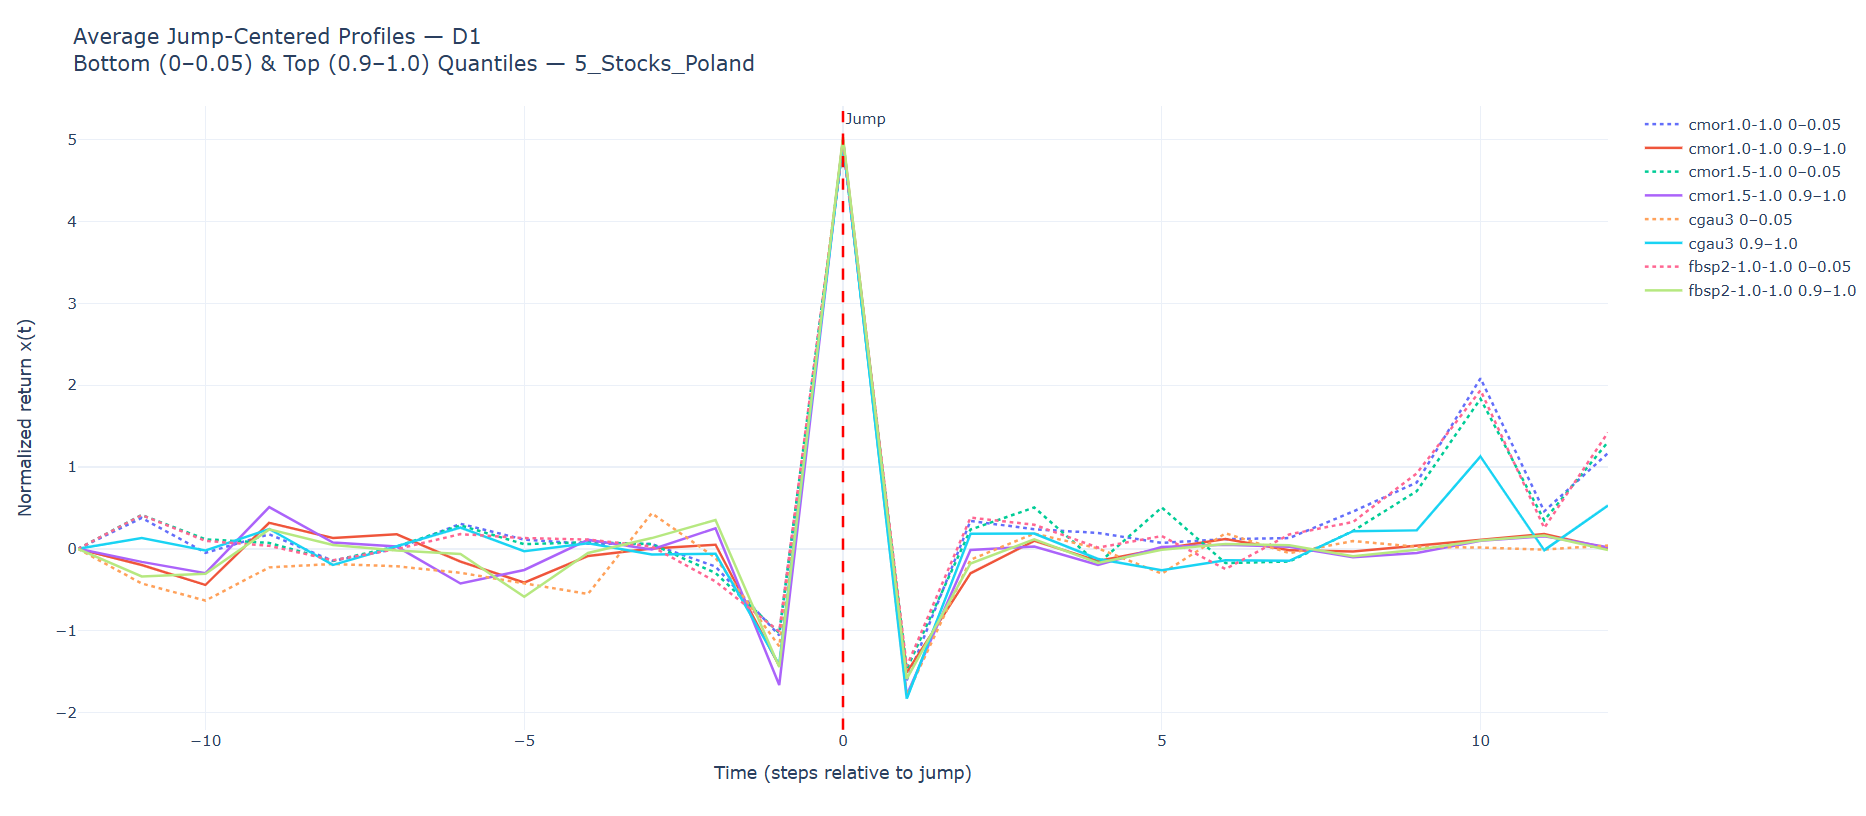
\includegraphics[width=\textwidth]{D1_different_wavelets.png}
        \caption{First KPCA direction}
    \end{subfigure}
    \hfill
    \begin{subfigure}[b]{0.32\textwidth}
        \centering
        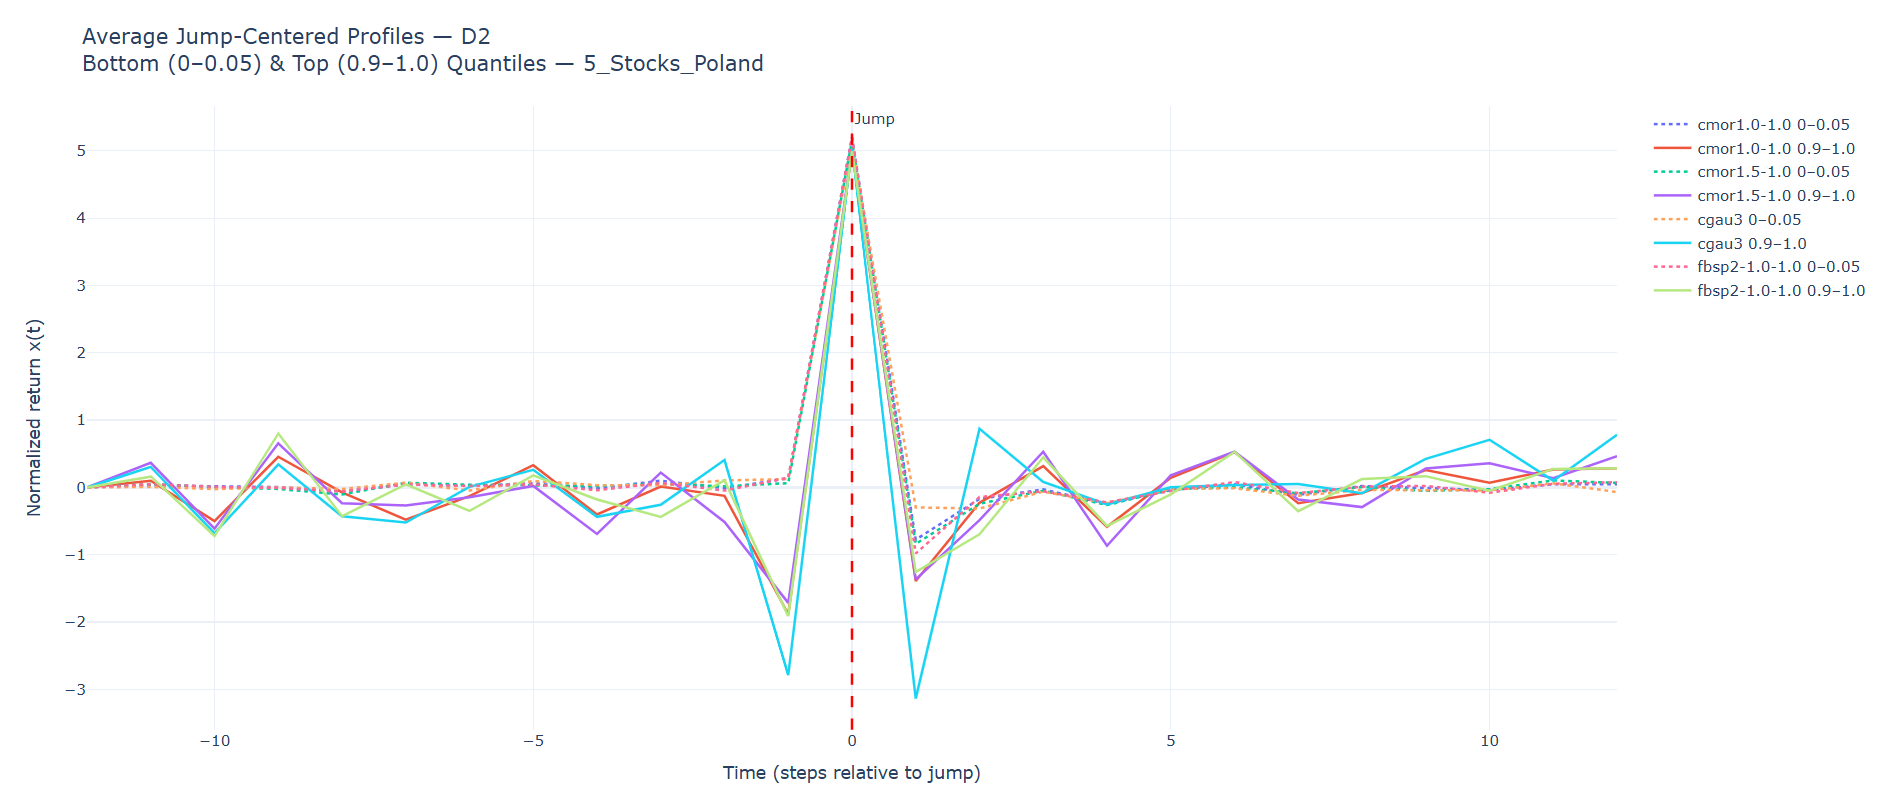
\includegraphics[width=\textwidth]{D2_different_wavelets.png}
        \caption{Second KPCA direction}
    \end{subfigure}
    \hfill
    \begin{subfigure}[b]{0.32\textwidth}
        \centering
        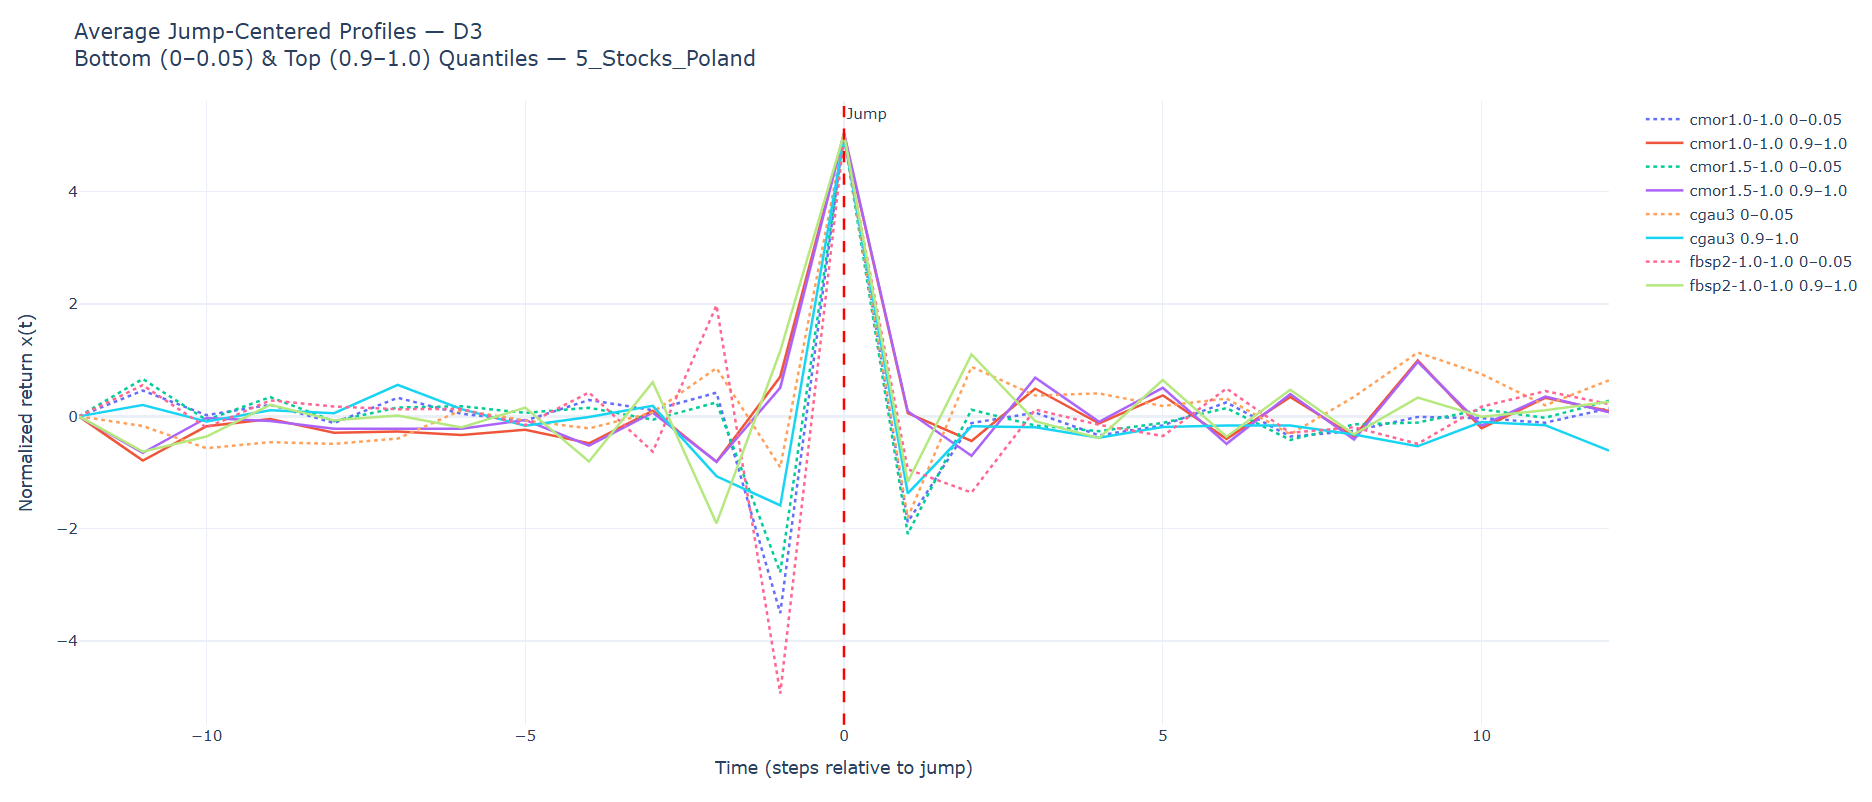
\includegraphics[width=\textwidth]{D3_different_wavelets.png}
        \caption{Third KPCA direction}
    \end{subfigure}
    \caption{Visulization of first and last quantiles jumps on Poland stock data for wavelets: 2 complex Morlet (cmor), 1 complex Guassian (cgau) and a frequency B spline (fbsp).}
    \label{fig:wavelet_quantiles}
\end{figure}

\subsection{Threshold sweep overlays across frequencies}
This supplementary appendix provides the full set of threshold-sweep overlay plots across sampling frequencies (5-min, hourly, daily) for the three main directions ($D_1$, $D_2$, $D_3$). The main report includes the 5-min overlays; the plots below show the complete comparison grid.

\begin{figure}[H]
\centering
\begin{subfigure}{0.32\textwidth}
    \centering
    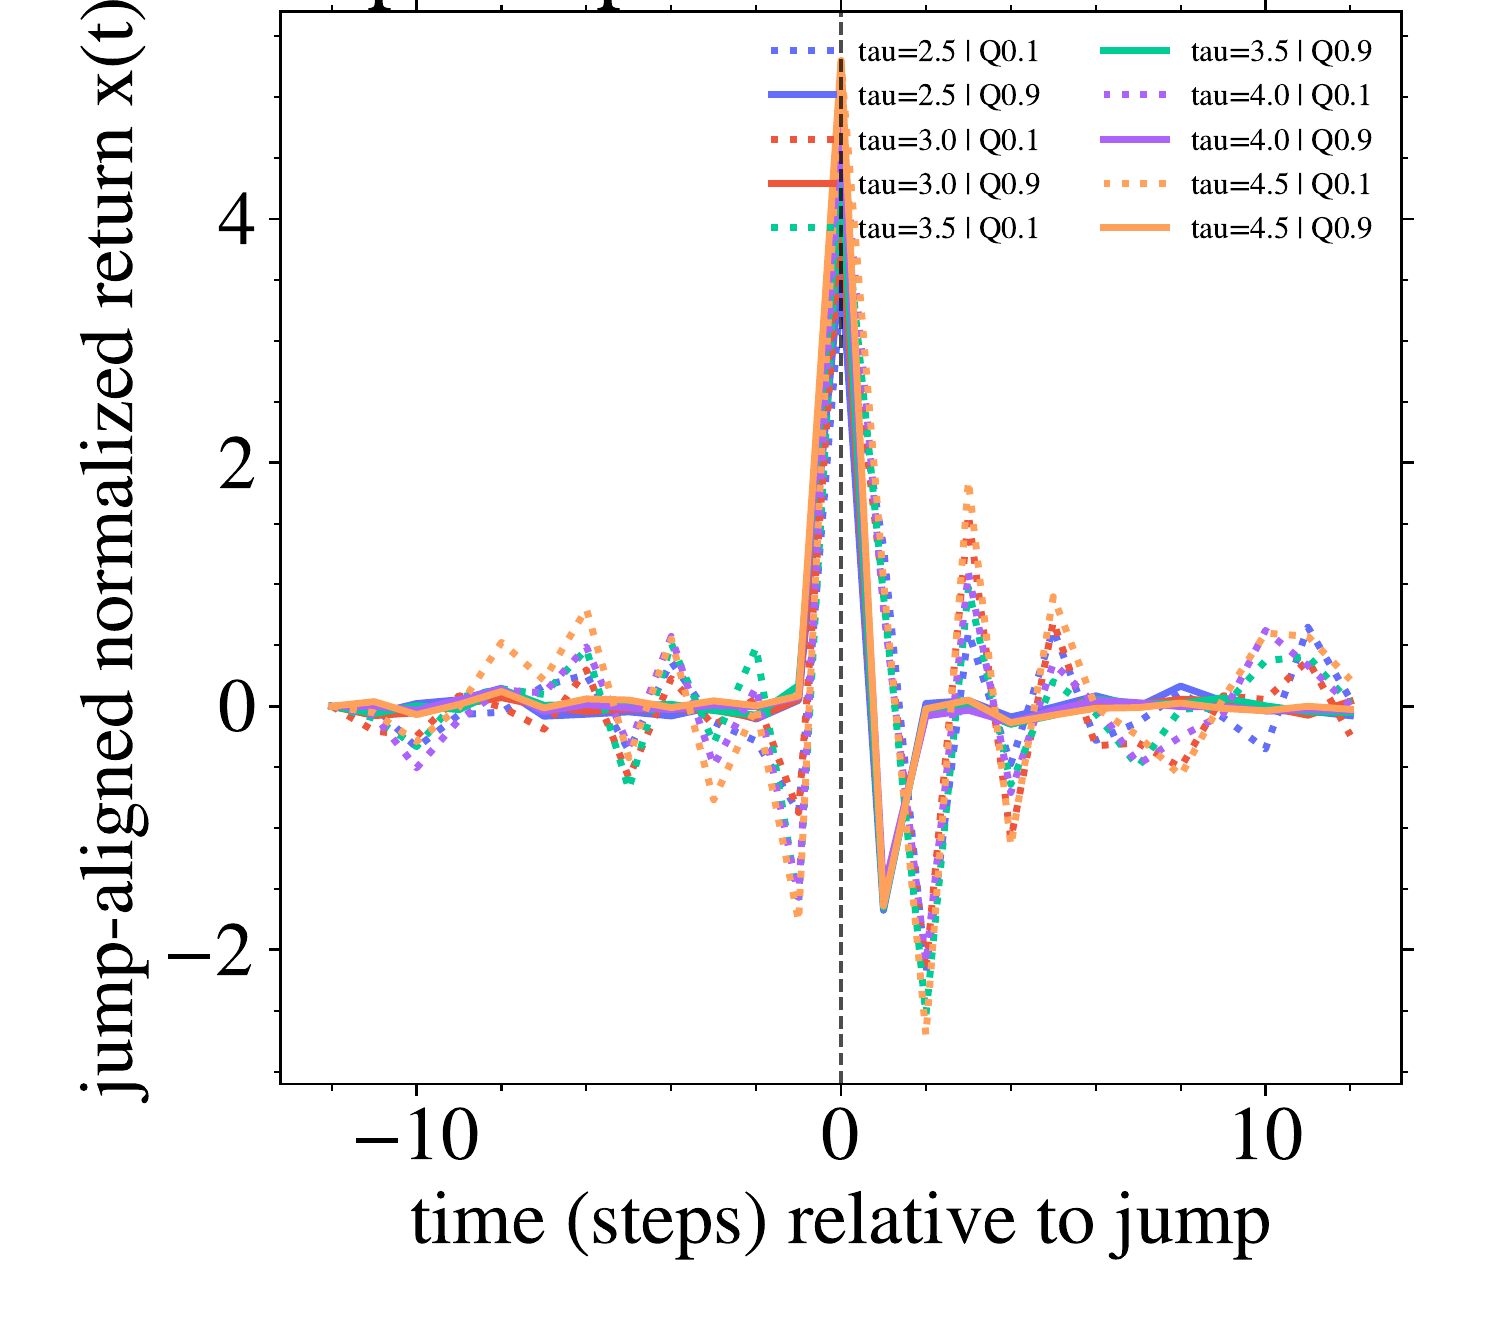
\includegraphics[width=\textwidth]{figures/2/overlay_D1_thresholds_5min_mpl.png}
    \caption{$D_1$ (5-min)}
\end{subfigure}
\begin{subfigure}{0.32\textwidth}
    \centering
    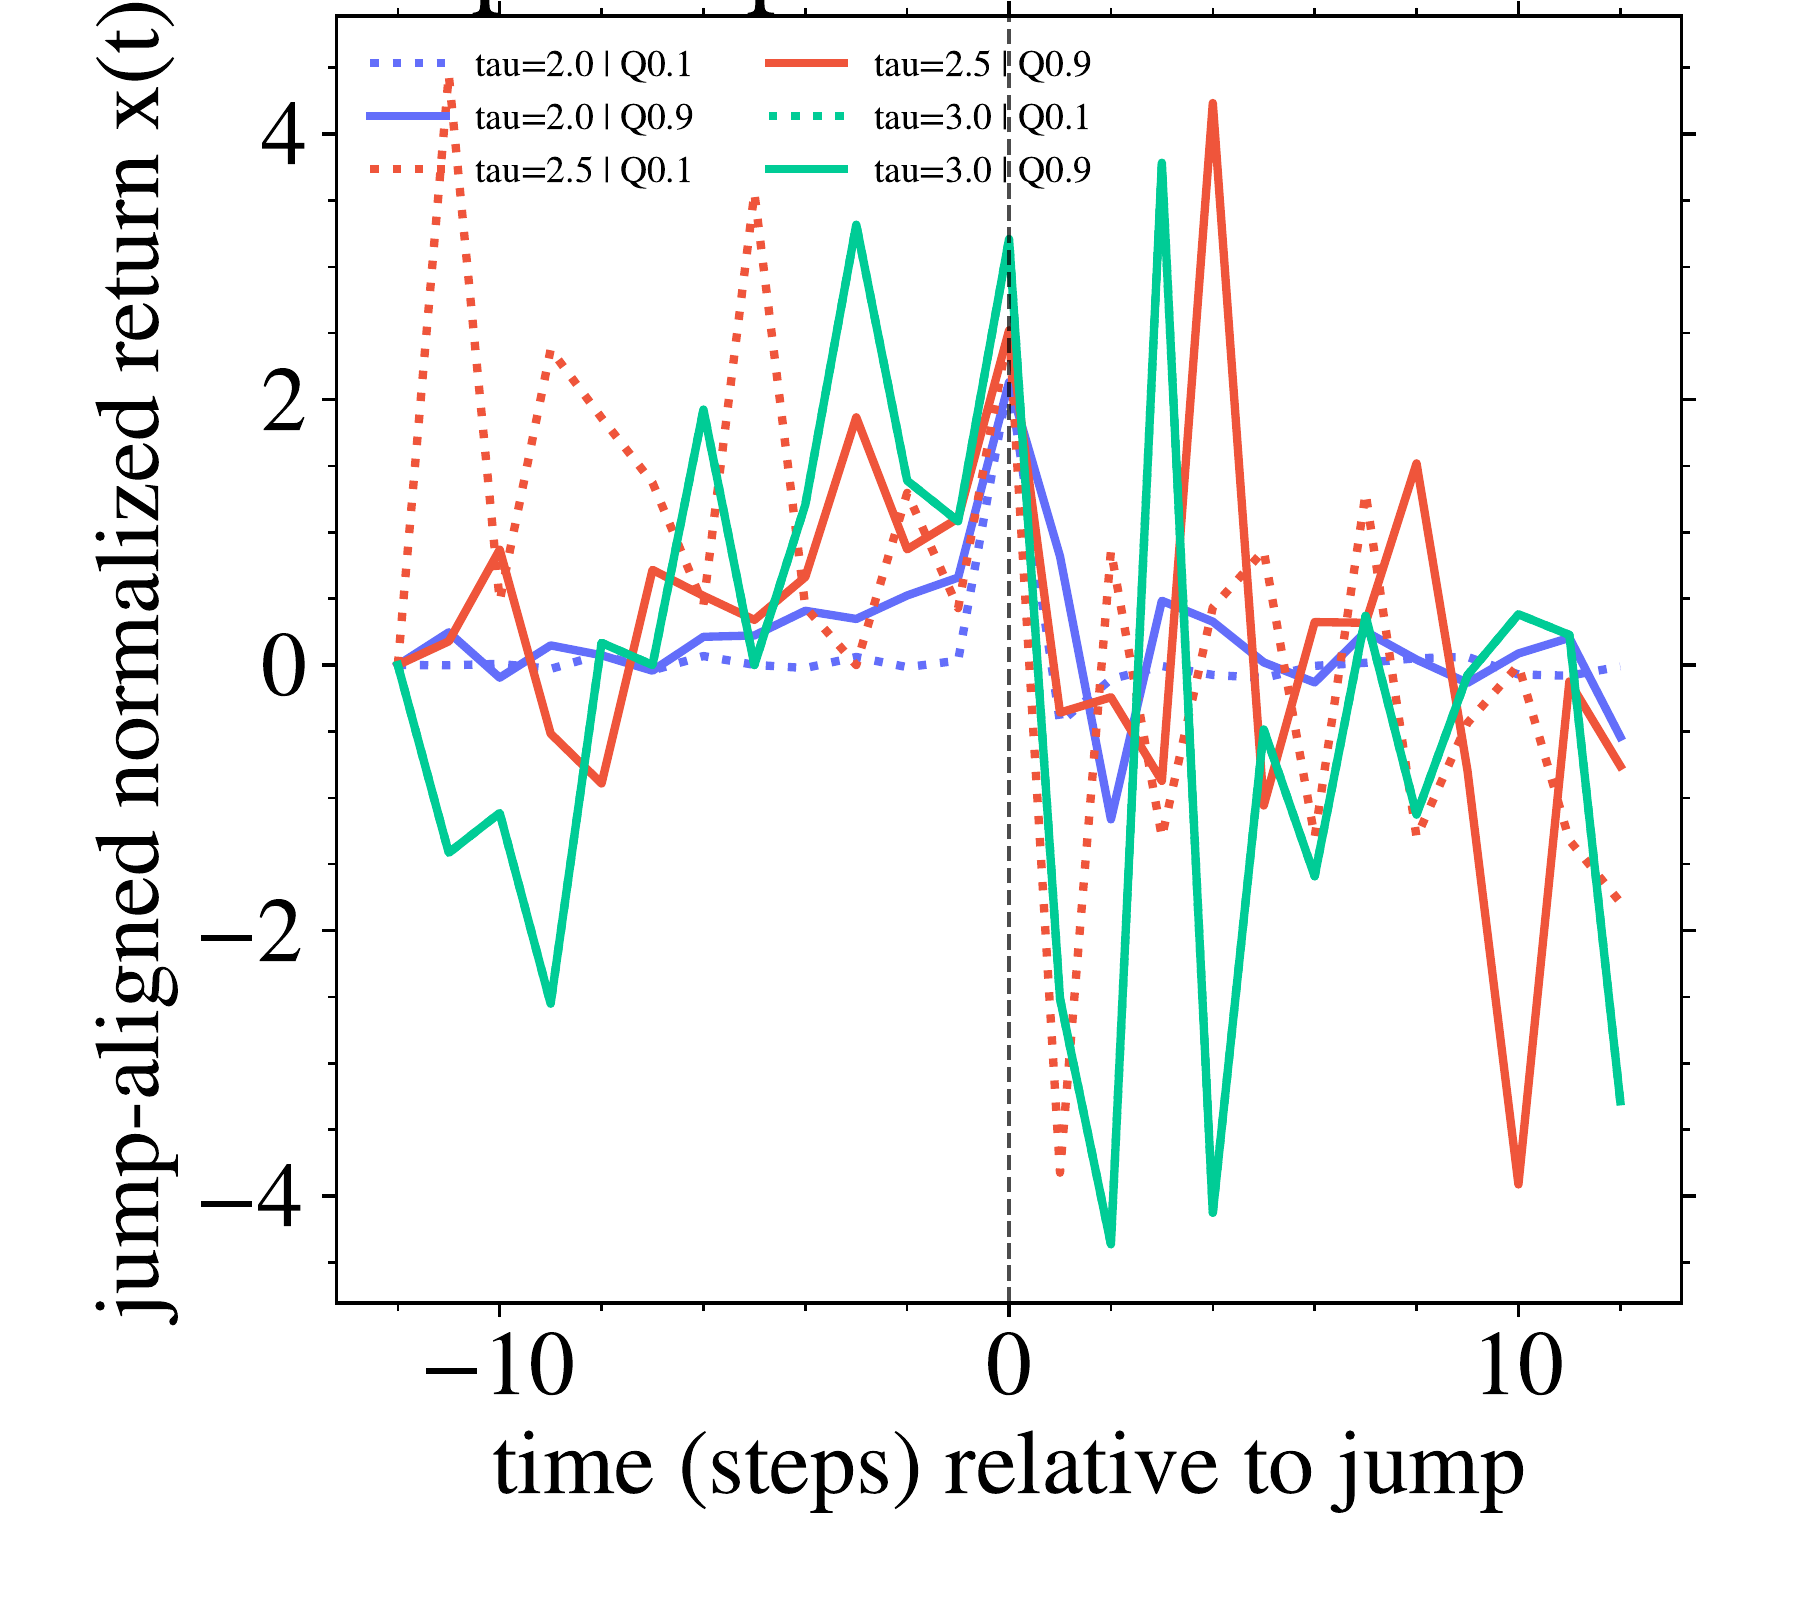
\includegraphics[width=\textwidth]{figures/2/overlay_D1_thresholds_hourly_mpl.png}
    \caption{$D_1$ (hourly)}
\end{subfigure}
\begin{subfigure}{0.32\textwidth}
    \centering
    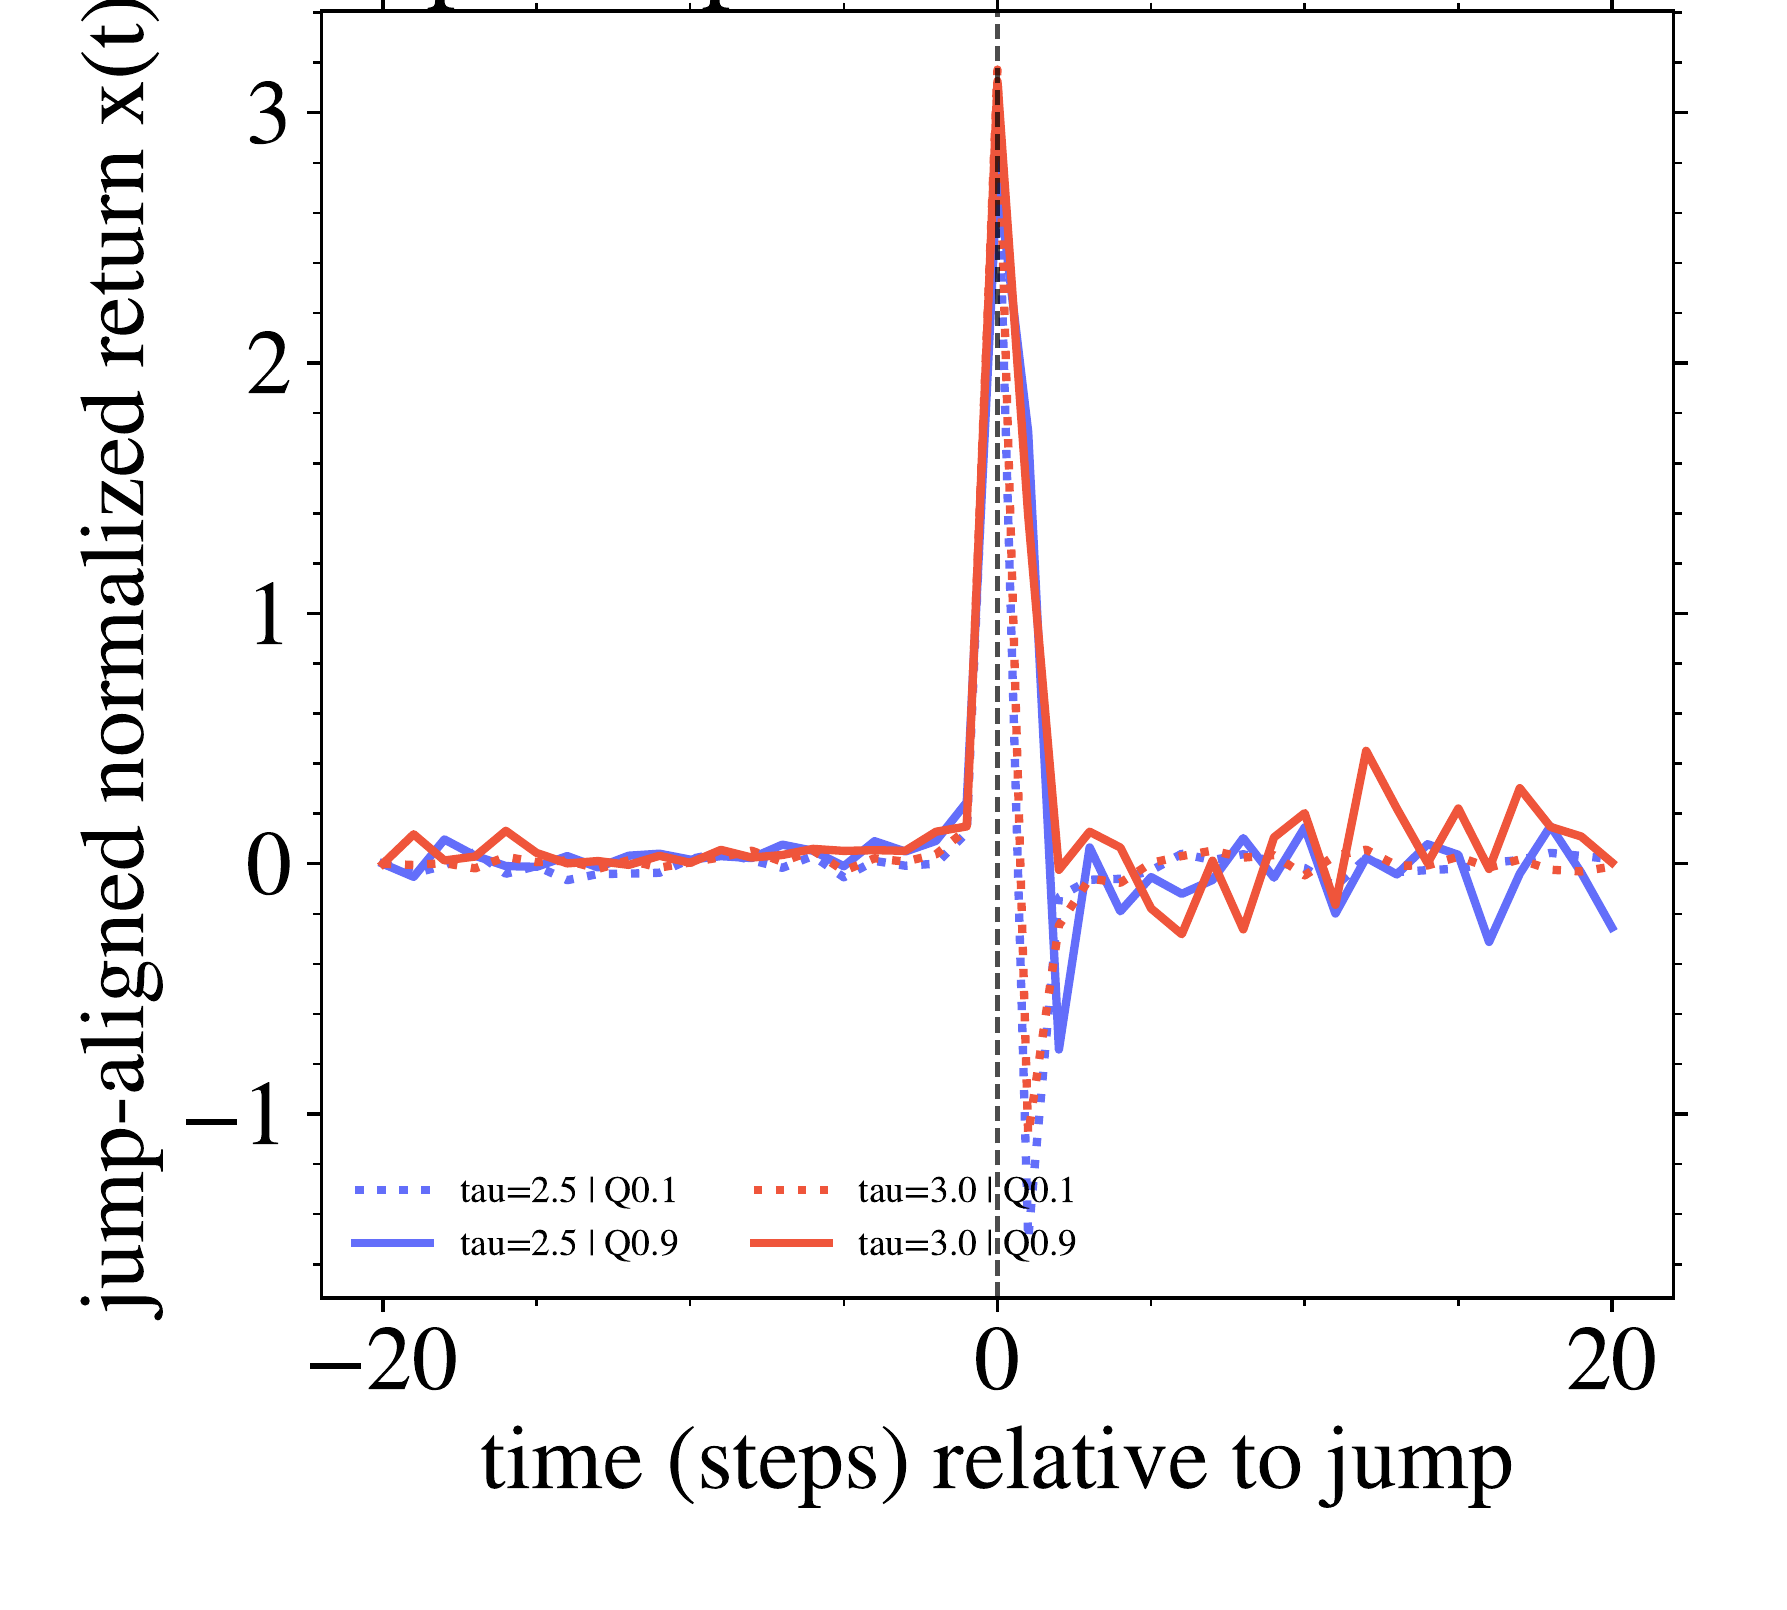
\includegraphics[width=\textwidth]{figures/2/overlay_D1_thresholds_daily_mpl.png}
    \caption{$D_1$ (daily)}
\end{subfigure}

\begin{subfigure}{0.32\textwidth}
    \centering
    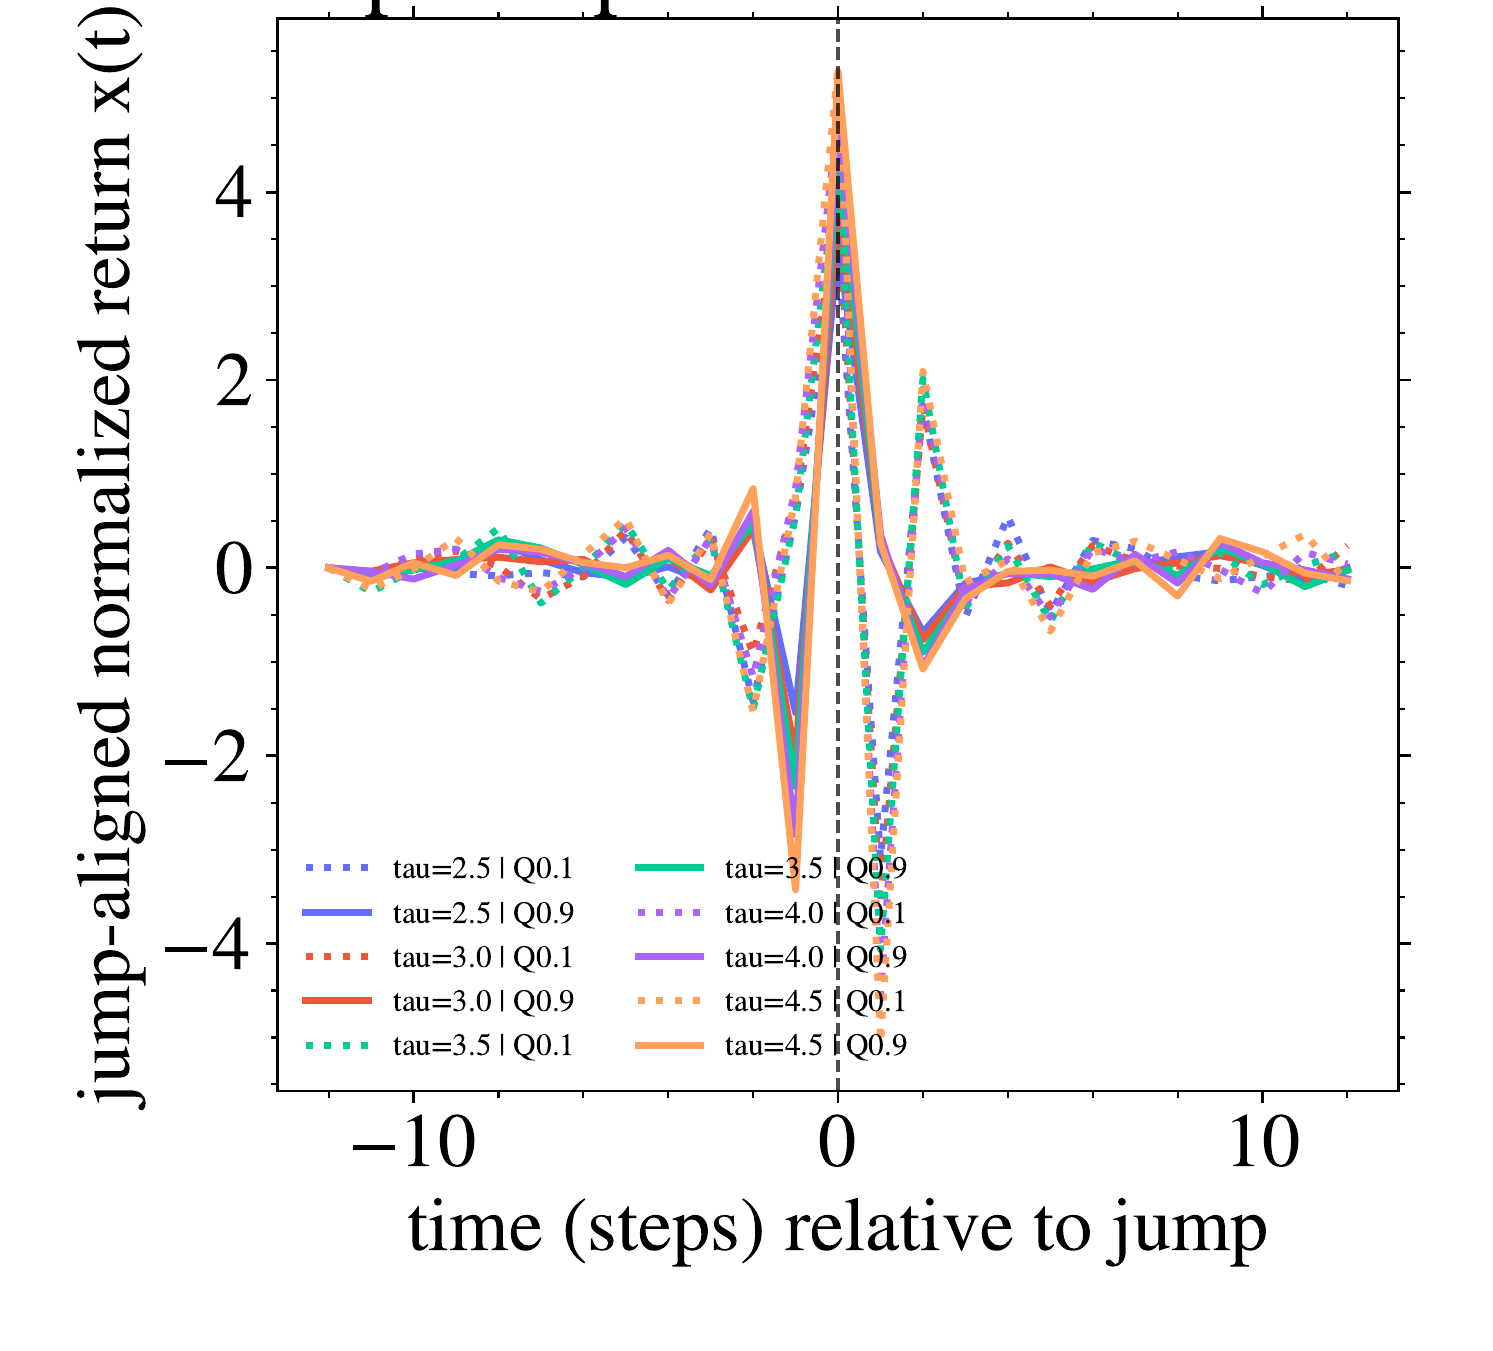
\includegraphics[width=\textwidth]{figures/2/overlay_D2_thresholds_5min_mpl.png}
    \caption{$D_2$ (5-min)}
\end{subfigure}
\begin{subfigure}{0.32\textwidth}
    \centering
    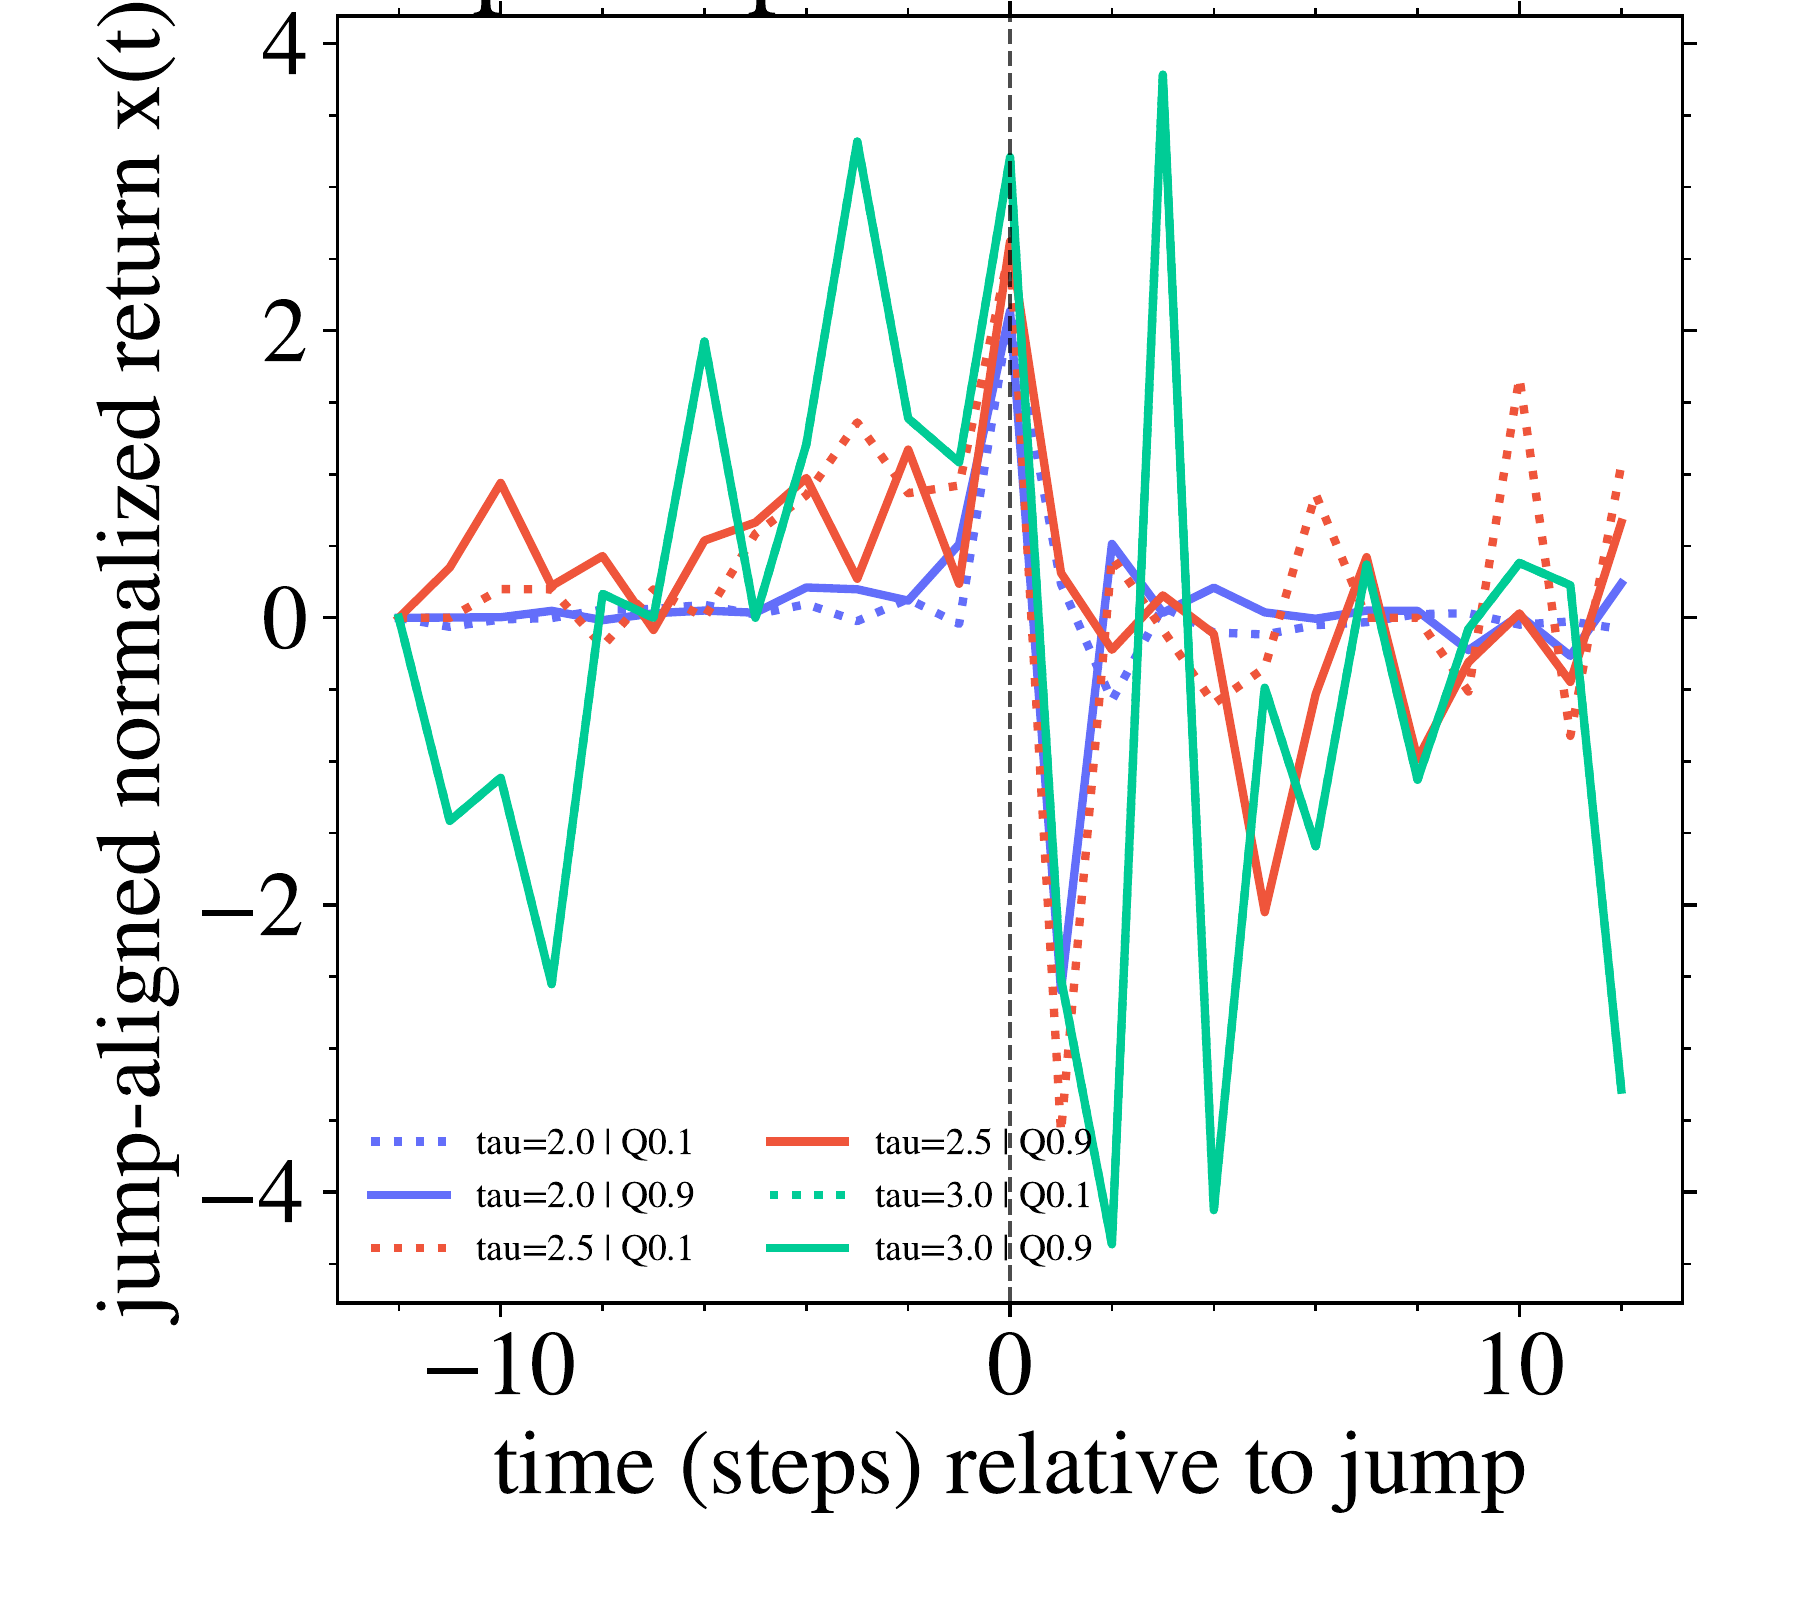
\includegraphics[width=\textwidth]{figures/2/overlay_D2_thresholds_hourly_mpl.png}
    \caption{$D_2$ (hourly)}
\end{subfigure}
\begin{subfigure}{0.32\textwidth}
    \centering
    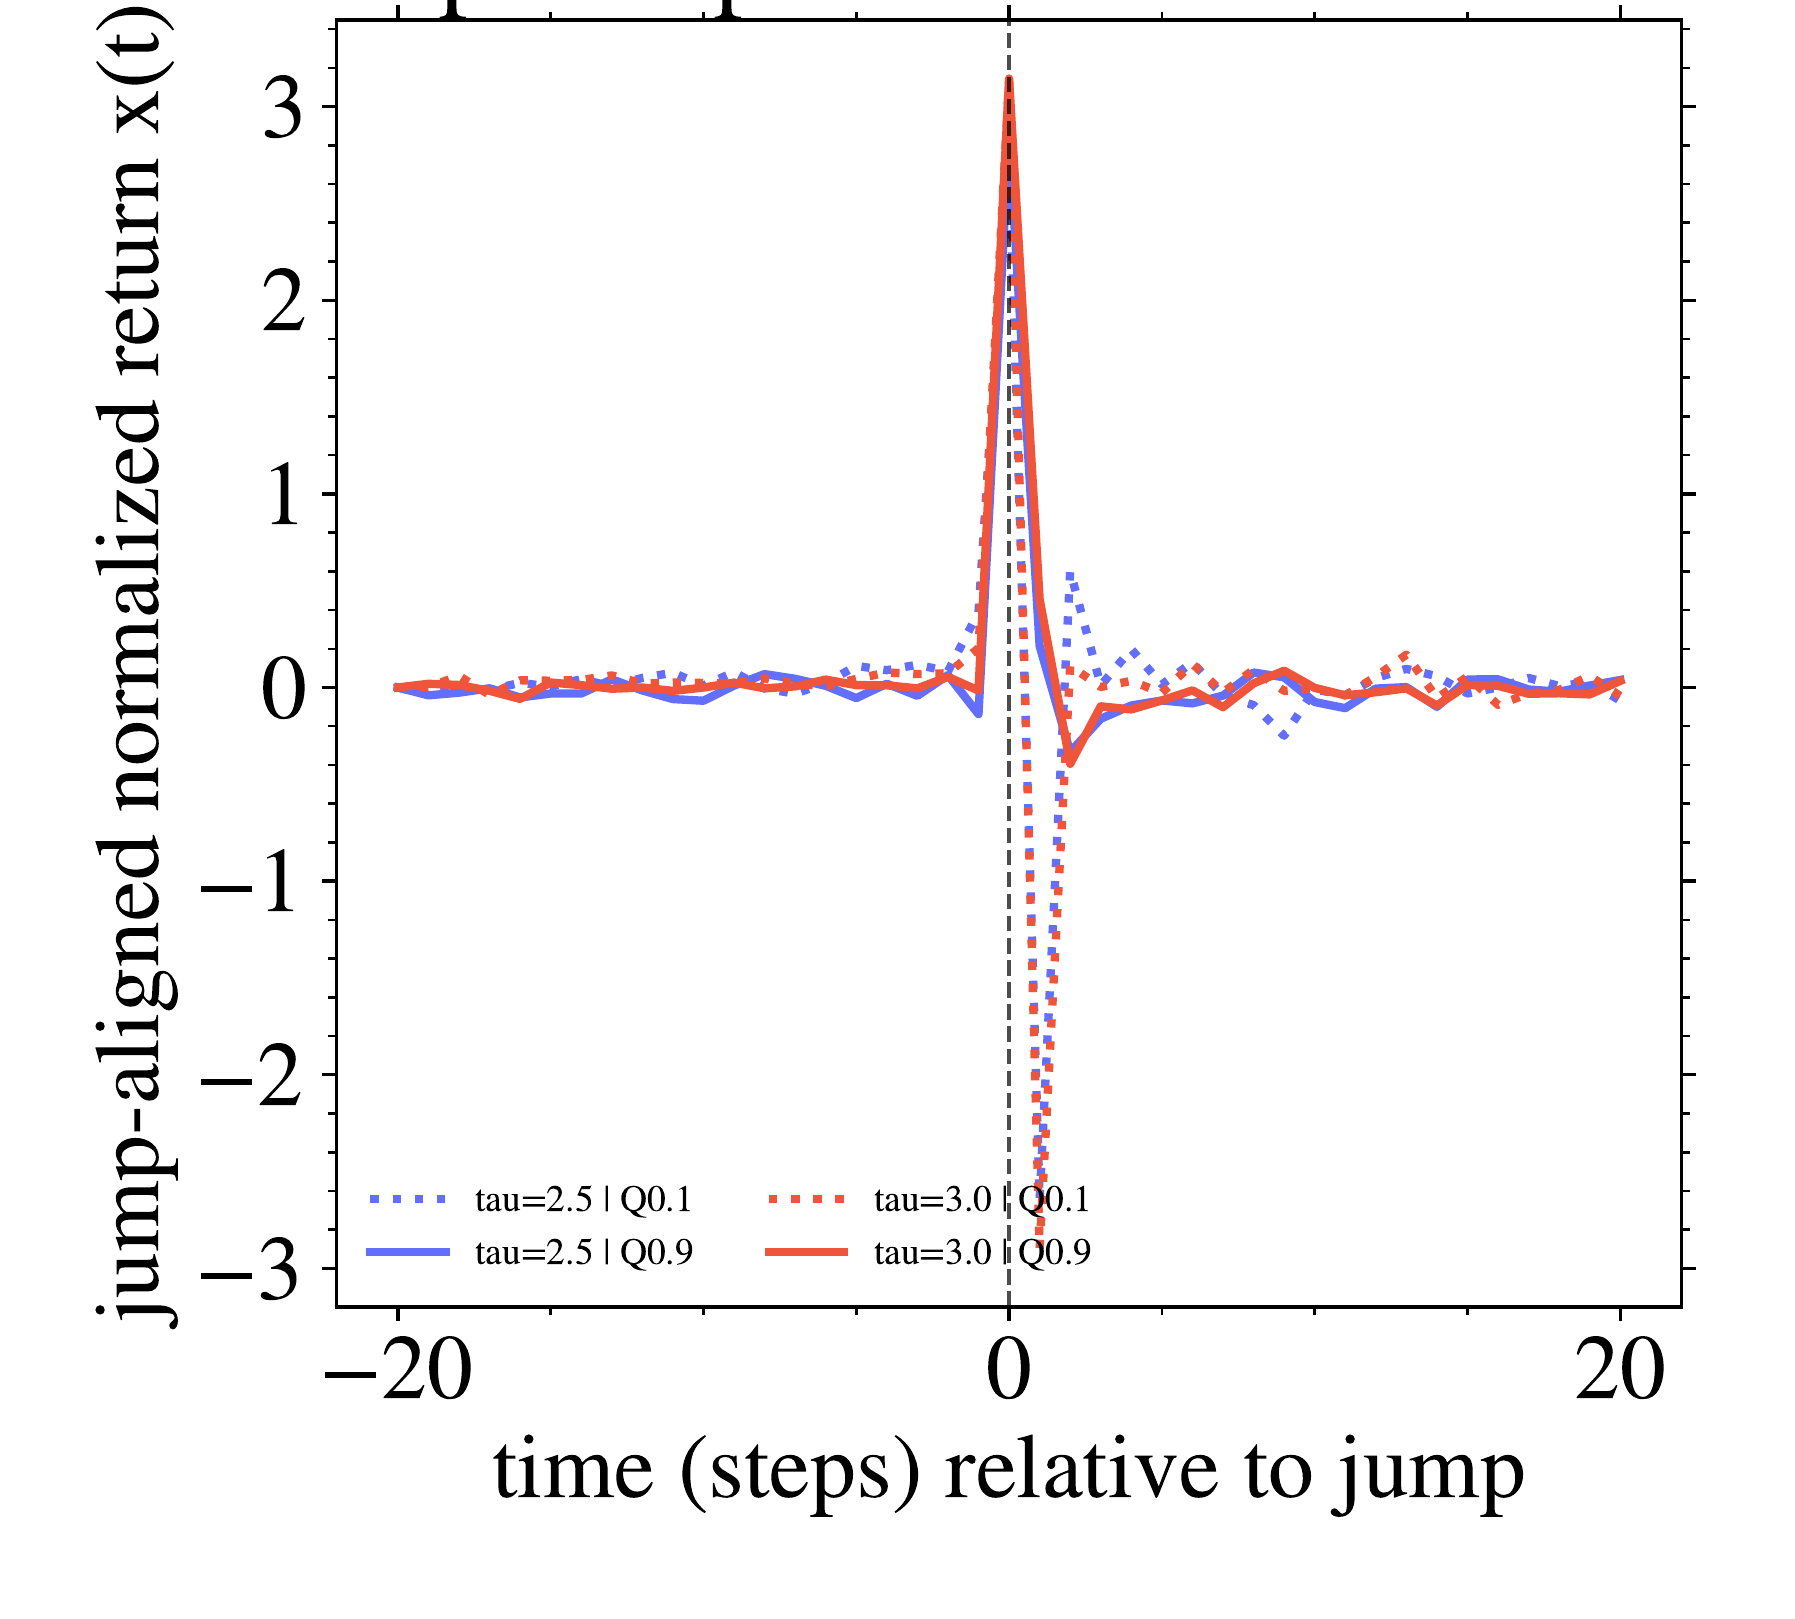
\includegraphics[width=\textwidth]{figures/2/overlay_D2_thresholds_daily_mpl.png}
    \caption{$D_2$ (daily)}
\end{subfigure}

\begin{subfigure}{0.32\textwidth}
    \centering
    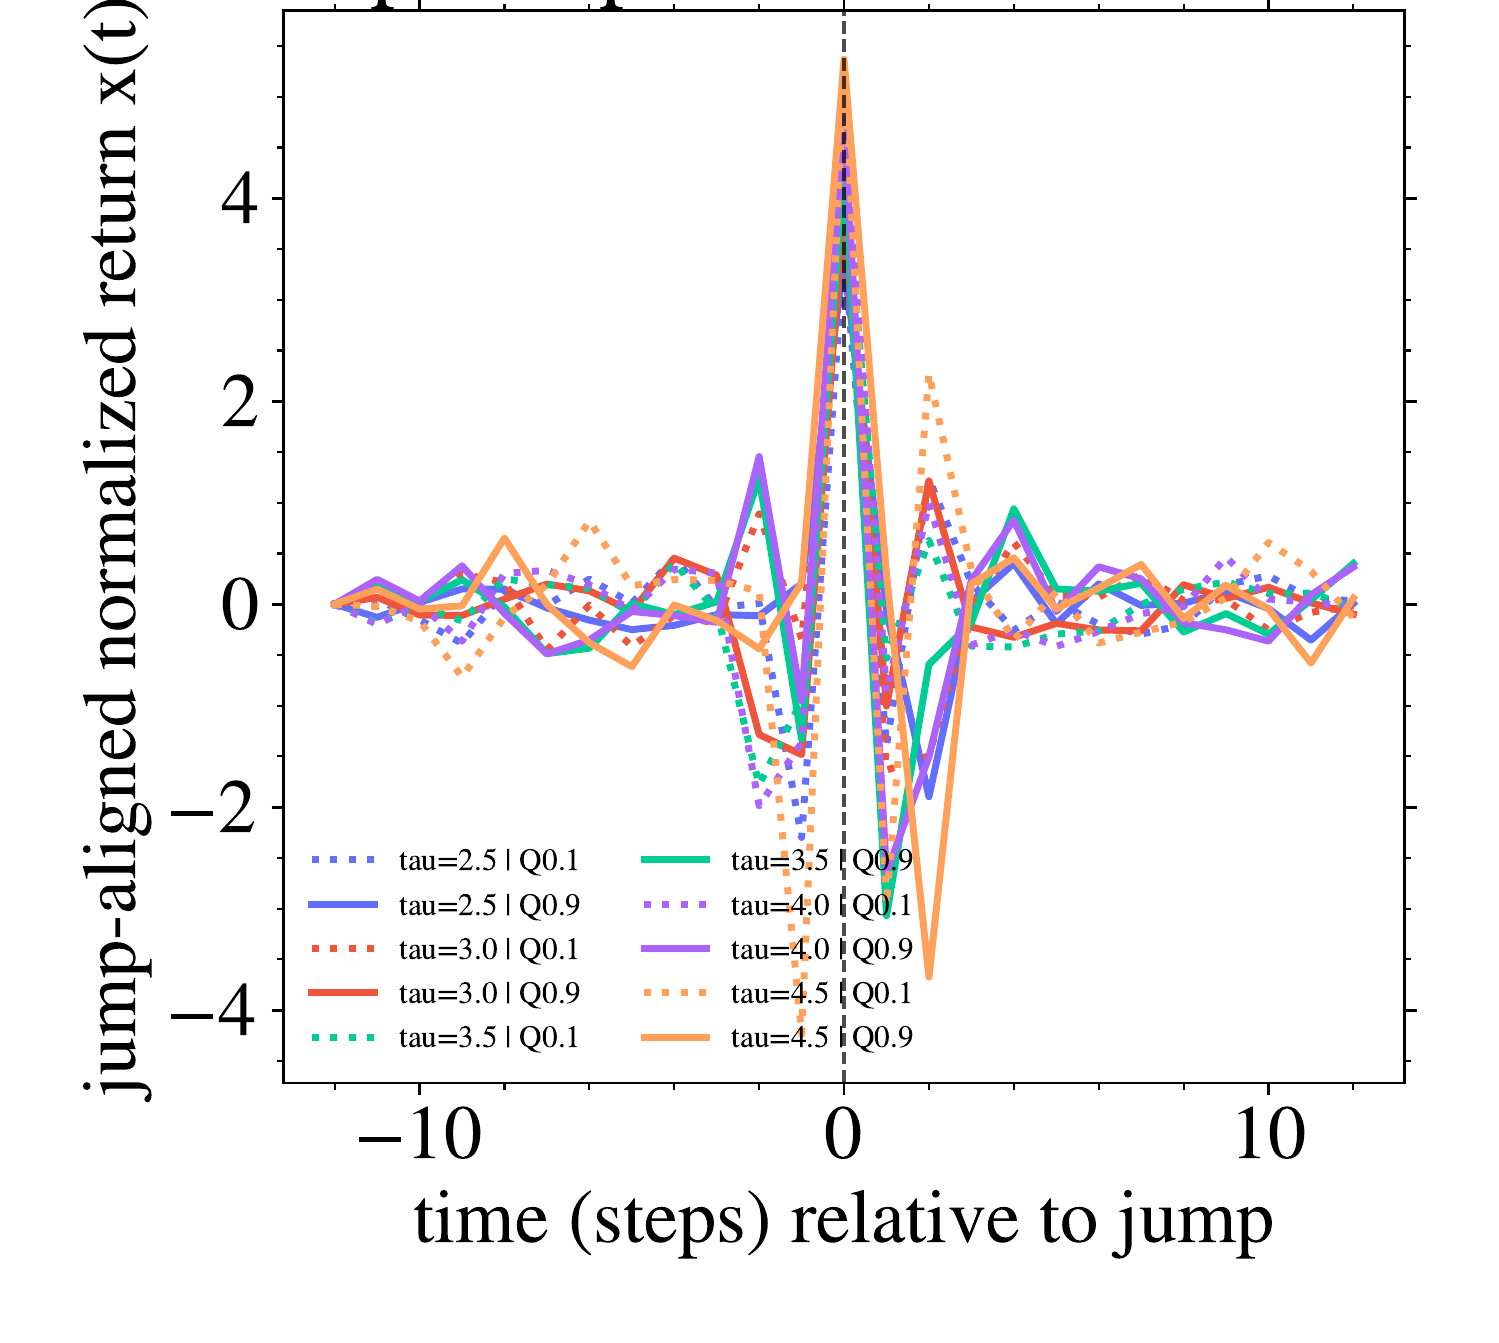
\includegraphics[width=\textwidth]{figures/2/overlay_D3_thresholds_5min_mpl.png}
    \caption{$D_3$ (5-min)}
\end{subfigure}
\begin{subfigure}{0.32\textwidth}
    \centering
    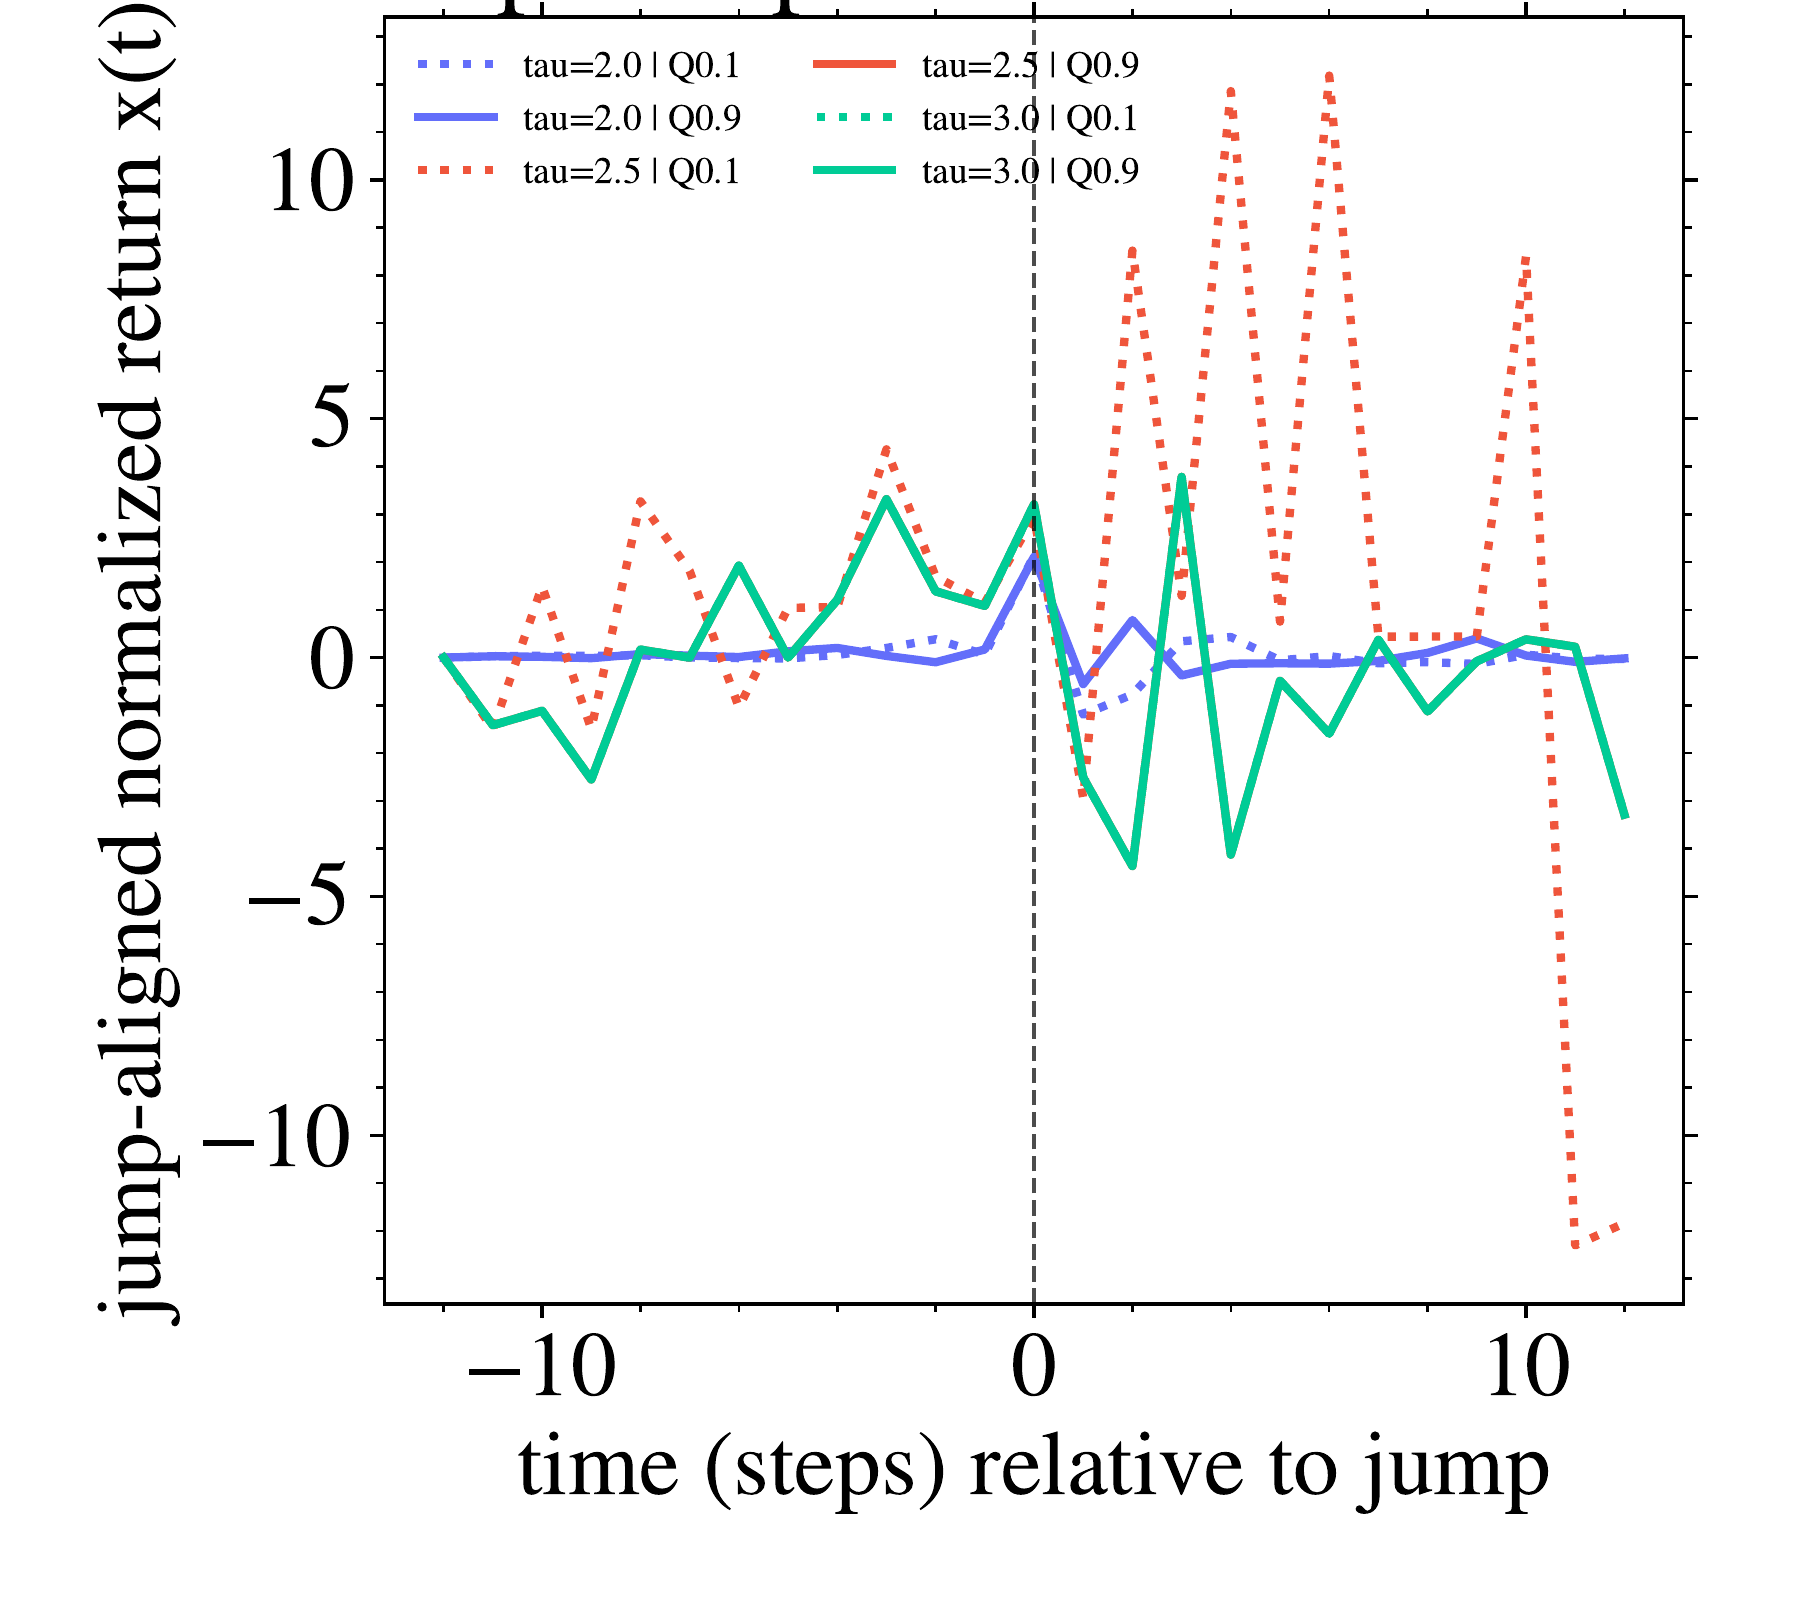
\includegraphics[width=\textwidth]{figures/2/overlay_D3_thresholds_hourly_mpl.png}
    \caption{$D_3$ (hourly)}
\end{subfigure}
\begin{subfigure}{0.32\textwidth}
    \centering
    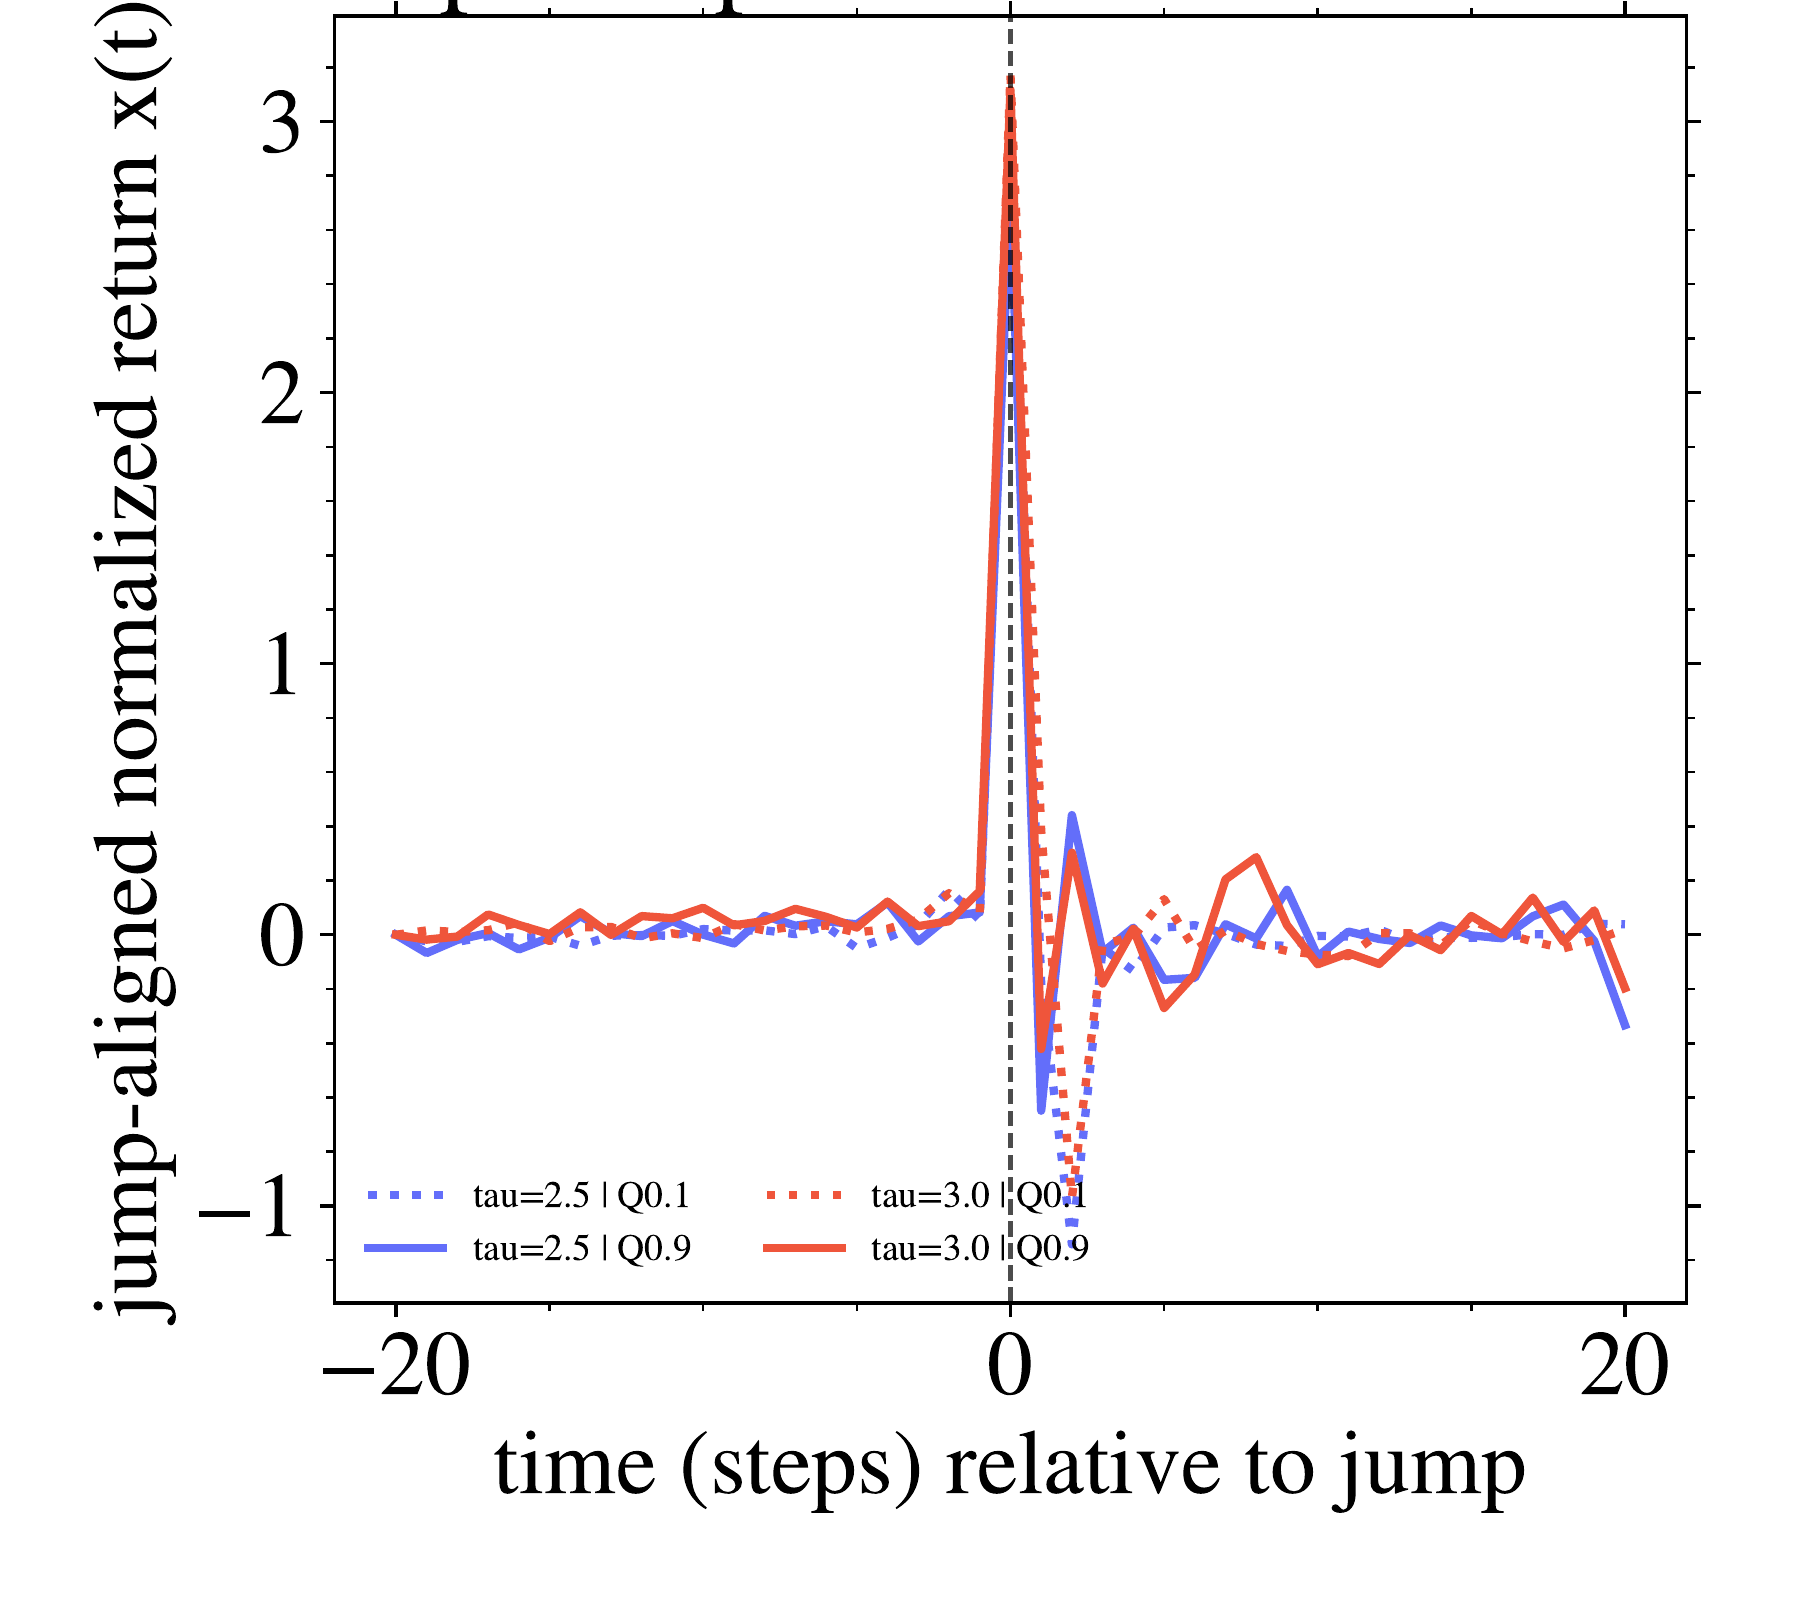
\includegraphics[width=\textwidth]{figures/2/overlay_D3_thresholds_daily_mpl.png}
    \caption{$D_3$ (daily)}
\end{subfigure}

\caption{Threshold sweep overlays across frequencies (5-min, hourly, daily).}
\label{fig:threshold_sweep_all}
\end{figure}





% \subsection{Jump Score Distribution}

% Figure~\ref{fig:jump_distribution} shows the distribution of standardized returns $x(t)$ and the fit to a Gumbel distribution for the upper tail (quantiles $> 0.28$). The Q-Q plot in Figure~\ref{fig:qq_plot} confirms the Gumbel distribution is a good fit for the tail region.

% \begin{figure}[H]
% \centering
% \begin{subfigure}{0.48\textwidth}
%     \centering
%     
\includegraphics[width=\textwidth]{figures/jump_density_poland_distribution_signed.pdf}
%     \caption{Distribution of signed standardized returns}
%     \label{fig:dist_signed}
% \end{subfigure}
% \begin{subfigure}{0.48\textwidth}
%     \centering
%     
\includegraphics[width=\textwidth]{figures/jump_density_poland_distribution_abs.pdf}
%     \caption{Distribution of absolute standardized returns with Gumbel fit}
%     \label{fig:dist_abs}
% \end{subfigure}
% \caption{Distribution of standardized returns $x(t)$ for Poland dataset}
% \label{fig:jump_distribution}
% \end{figure}

% \begin{figure}[H]
% \centering
% 
\includegraphics[width=0.7\textwidth]{figures/jump_density_poland_qq_plot.pdf}
% \caption{Q-Q plot comparing empirical quantiles to Gumbel distribution (quantiles 0.28-1.0)}
% \label{fig:qq_plot}
% \end{figure}

% \subsection{PCA Directions}

% \subsubsection{D1: Reflexivity}

% Figure~\ref{fig:d1_asymmetry} shows the correlation between $D_1$ (reflexivity) and the asymmetry measure $\mathcal{A}_{\text{jump}} = (\mathcal{A}_{>} - \mathcal{A}_{<})/(\mathcal{A}_{>} + \mathcal{A}_{<})$. The strong positive correlation confirms that $D_1$ captures volatility asymmetry.

% \begin{figure}[H]
% \centering
% 
\includegraphics[width=0.7\textwidth]{figures/reproduce_poland_D1_asymmetry.pdf}
% \caption{D1 (Reflexivity) vs Asymmetry measure. Positive correlation confirms D1 captures time-asymmetry of volatility.}
% \label{fig:d1_asymmetry}
% \end{figure}

% \subsubsection{D1 vs D2: Mean-Reversion}

% Figure~\ref{fig:d1_d2} shows the 2D projection of jumps onto the reflexivity ($D_1$) and mean-reversion ($D_2$) directions. This reveals different classes of jumps: endogenous (negative $D_1$), exogenous (positive $D_1$), and mean-reverting (large $|D_2|$).

% \begin{figure}[H]
% \centering
% 
\includegraphics[width=0.7\textwidth]{figures/reproduce_poland_fig5_mr.pdf}
% \caption{2D projection: Reflexivity ($D_1$) vs Mean-Reversion ($D_2$)}
% \label{fig:d1_d2}
% \end{figure}

% \subsubsection{D1 vs D3: Trend}

% Figure~\ref{fig:d1_d3} shows the projection onto reflexivity and trend directions, revealing trend-aligned and trend-anti-aligned jumps.

% \begin{figure}[H]
% \centering
% 
\includegraphics[width=0.7\textwidth]{figures/reproduce_poland_fig6_tr.pdf}
% \caption{2D projection: Reflexivity ($D_1$) vs Trend ($D_3$)}
% \label{fig:d1_d3}
% \end{figure}

% \subsection{Average Profiles}

% Figure~\ref{fig:profiles_d1} shows average temporal profiles along the $D_1$ direction, confirming that:
% \begin{itemize}
%     \item Negative $D_1$ (left): Anticipatory jumps with pre-jump activity
%     \item Near zero $D_1$ (center): Endogenous jumps with symmetric profiles
%     \item Positive $D_1$ (right): Exogenous jumps with post-jump activity
% \end{itemize}

% \begin{figure}[H]
% \centering
% 
\includegraphics[width=0.9\textwidth]{figures/reproduce_poland_profile_D1_reflexivity.pdf}
% \caption{Average profiles along D1 (Reflexivity) direction, sliced into quantile bins}
% \label{fig:profiles_d1}
% \end{figure}

% Similar profiles for $D_2$ and $D_3$ are shown in Figures~\ref{fig:profiles_d2} and~\ref{fig:profiles_d3}.

% \begin{figure}[H]
% \centering
% \begin{subfigure}{0.48\textwidth}
%     \centering
%     
\includegraphics[width=\textwidth]{figures/reproduce_poland_profile_D2_mean_reversion.pdf}
%     \caption{Mean-Reversion ($D_2$)}
%     \label{fig:profiles_d2}
% \end{subfigure}
% \begin{subfigure}{0.48\textwidth}
%     \centering
%     
\includegraphics[width=\textwidth]{figures/reproduce_poland_profile_D3_trend.pdf}
%     \caption{Trend ($D_3$)}
%     \label{fig:profiles_d3}
% \end{subfigure}
% \caption{Average temporal profiles along D2 and D3 directions}
% \label{fig:profiles_d2_d3}
% \end{figure}

% \subsection{Example Jumps}

% Figure~\ref{fig:example_jumps} shows examples of endogenous and exogenous jumps from the dataset, including their normalized profiles and actual price/return series.

% % \begin{figure}[H]
% % \centering
% % \includegraphics[width=0.9\textwidth]{figures/jump_density_poland_examples.pdf}
% % \caption{Example endogenous and exogenous jumps from the dataset. Top row shows $|x(t)|$ profiles, bottom row shows $x(t)$ profiles.}
% % \label{fig:example_jumps}
% % \end{figure}

% \subsection{Scattering Spectra Comparison}

% We compare results with and without Scattering Spectra features. Figure~\ref{fig:ss_comparison_d1} shows that including SS features does not significantly alter the $D_1$ direction (correlation $> 0.95$), suggesting the base wavelet features are sufficient for capturing reflexivity.

% \begin{figure}[H]
% \centering
% \begin{subfigure}{0.48\textwidth}
%     \centering
%     
\includegraphics[width=\textwidth]{figures/poland_comparison_D1_scatter.pdf}
%     \caption{D1 scatter plot comparison}
%     \label{fig:ss_comparison_d1}
% \end{subfigure}
% \begin{subfigure}{0.48\textwidth}
%     \centering
%     
\includegraphics[width=\textwidth]{figures/poland_comparison_D1_distribution.pdf}
%     \caption{D1 distributions}
%     \label{fig:ss_comparison_d1_dist}
% \end{subfigure}
% \caption{Comparison of D1 with and without Scattering Spectra}
% \label{fig:ss_comparison_d1_full}
% \end{figure}

% Similar comparisons for $D_2$ and $D_3$ are shown in Figures~\ref{fig:ss_comparison_d2} and~\ref{fig:ss_comparison_d3}.

% \begin{figure}[H]
% \centering
% \begin{subfigure}{0.48\textwidth}
%     \centering
%     
\includegraphics[width=\textwidth]{figures/poland_comparison_D2_scatter.pdf}
%     \caption{D2 scatter plot comparison}
%     \label{fig:ss_comparison_d2}
% \end{subfigure}
% \begin{subfigure}{0.48\textwidth}
%     \centering
%     
\includegraphics[width=\textwidth]{figures/poland_comparison_D3_scatter.pdf}
%     \caption{D3 scatter plot comparison}
%     \label{fig:ss_comparison_d3}
% \end{subfigure}
% \caption{Comparison of D2 and D3 with and without Scattering Spectra}
% \label{fig:ss_comparison_d2_d3}
% \end{figure}

% \section{Multi-Stock Analysis}

% We analyze the dependence on the number of stocks and data quantity. Figure~\ref{fig:multi_stock} shows results for different subsets of stocks.

% % \begin{figure}[H]
% % \centering
% % \begin{subfigure}{0.48\textwidth}
% %     \centering
% %     \includegraphics[width=\textwidth]{figures/reproduce_poland_5_Stocks_Poland_fig5_mr.pdf}
% %     \caption{5 stocks}
% % \end{subfigure}
% % \begin{subfigure}{0.48\textwidth}
% %     \centering
% %     \includegraphics[width=\textwidth]{figures/reproduce_poland_30_Stocks_Poland_fig5_mr.pdf}
% %     \caption{30 stocks}
% % \end{subfigure}
% % \caption{D1 vs D2 projections for different numbers of stocks (Poland dataset). The patterns are consistent across different data quantities.}
% % \label{fig:multi_stock}
% % \end{figure}

% \section{Discussion}

% Our implementation successfully reproduces the main findings of the paper:
% \begin{enumerate}
%     \item The jump score $|x(t)|$ follows a Gumbel distribution in the tail region
%     \item The first PCA direction $D_1$ captures volatility asymmetry (reflexivity)
%     \item Mean-reversion ($D_2$) and trend ($D_3$) are important additional features
%     \item The methodology identifies endogenous, exogenous, and anticipatory jumps
% \end{enumerate}

% The inclusion of Scattering Spectra features does not significantly alter the discovered directions, suggesting that the base wavelet scattering coefficients are sufficient for this classification task.

% \section{Conclusion}

% We have successfully implemented and validated the wavelet-based jump classification methodology. The code is available in the \texttt{notebooks/jump/} directory and can be applied to different markets (Poland, Hong Kong) and datasets.

% Future work could include:
% \begin{itemize}
%     \item Extension to co-jump analysis
%     \item Application to higher frequency data
%     \item Comparison with other classification methods
%     \item Analysis of market-specific patterns
% \end{itemize}



\end{document}

